% =====================================================================
% StaticKD -- naskah jurnal (bahasa Indonesia; istilah teknis bahasa Inggris dipertahankan)
% Format : IEEEtran (journal), target IEEE Access
% Kompil : pdflatex main && bibtex main && pdflatex main && pdflatex main
% Angka  : SEMUA angka hasil berasal dari generated/numbers.tex dan generated/tab_*.tex yang
%          ditulis oleh notebooks/StaticKD_IPTC_final.ipynb (Bagian 11). Jangan diketik manual.
% =====================================================================
\documentclass[journal]{IEEEtran}

\usepackage[T1]{fontenc}
\usepackage[utf8]{inputenc}
\usepackage{cite}
\usepackage{amsmath,amssymb}
\usepackage{graphicx}
\usepackage{booktabs}
\usepackage{multirow}
\usepackage{array}
\usepackage{xcolor}
\usepackage[hyphens]{url}
\usepackage{tikz}
\usetikzlibrary{positioning,arrows.meta,fit,calc}

\renewcommand{\abstractname}{Abstrak}
\renewcommand{\IEEEkeywordsname}{Kata Kunci}
\renewcommand{\figurename}{Gbr.}
\renewcommand{\tablename}{Tabel}
\renewcommand{\refname}{Referensi}

\DeclareRobustCommand{\todo}[1]{{\color{red}[TODO: #1]}}
\newcommand{\eng}[1]{\textit{#1}}   % istilah bahasa Inggris dicetak miring, tidak diterjemahkan
\makeatletter
\newcommand{\rows}[1]{\@@input #1 } % isi baris tabel dari file (primitif, aman di dalam tabular)
\makeatother
% Generated by notebooks/StaticKD_IPTC_final.ipynb -- do not edit by hand.
\makeatletter
\providecommand{\val}[1]{\ifcsname val@#1\endcsname\csname val@#1\endcsname\else{\color{red}??}\fi}
\expandafter\def\csname val@abl.bigram.dev_macro\endcsname{0,754}
\expandafter\def\csname val@abl.bigram.dev_macro.delta\endcsname{$-$0,000}
\expandafter\def\csname val@abl.bigram.dev_macro.p\endcsname{1,000}
\expandafter\def\csname val@abl.bigram.dev_macro.sd\endcsname{0,008}
\expandafter\def\csname val@abl.bigram.heldout_acc\endcsname{0,811}
\expandafter\def\csname val@abl.bigram.heldout_acc.delta\endcsname{+0,003}
\expandafter\def\csname val@abl.bigram.heldout_acc.p\endcsname{0,352}
\expandafter\def\csname val@abl.bigram.heldout_acc.sd\endcsname{0,002}
\expandafter\def\csname val@abl.bigram.test_acc\endcsname{0,643}
\expandafter\def\csname val@abl.bigram.test_acc.sd\endcsname{0,005}
\expandafter\def\csname val@abl.bigram.test_macro\endcsname{0,544}
\expandafter\def\csname val@abl.bigram.test_macro.delta\endcsname{+0,002}
\expandafter\def\csname val@abl.bigram.test_macro.p\endcsname{1,000}
\expandafter\def\csname val@abl.bigram.test_macro.sd\endcsname{0,002}
\expandafter\def\csname val@abl.conf.dev_macro\endcsname{0,759}
\expandafter\def\csname val@abl.conf.dev_macro.delta\endcsname{+0,004}
\expandafter\def\csname val@abl.conf.dev_macro.p\endcsname{1,000}
\expandafter\def\csname val@abl.conf.dev_macro.sd\endcsname{0,005}
\expandafter\def\csname val@abl.conf.heldout_acc\endcsname{0,809}
\expandafter\def\csname val@abl.conf.heldout_acc.delta\endcsname{+0,001}
\expandafter\def\csname val@abl.conf.heldout_acc.p\endcsname{0,392}
\expandafter\def\csname val@abl.conf.heldout_acc.sd\endcsname{0,001}
\expandafter\def\csname val@abl.conf.test_acc\endcsname{0,640}
\expandafter\def\csname val@abl.conf.test_acc.sd\endcsname{0,004}
\expandafter\def\csname val@abl.conf.test_macro\endcsname{0,543}
\expandafter\def\csname val@abl.conf.test_macro.delta\endcsname{+0,000}
\expandafter\def\csname val@abl.conf.test_macro.p\endcsname{1,000}
\expandafter\def\csname val@abl.conf.test_macro.sd\endcsname{0,003}
\expandafter\def\csname val@abl.data130k.dev_macro\endcsname{0,736}
\expandafter\def\csname val@abl.data130k.dev_macro.delta\endcsname{$-$0,019}
\expandafter\def\csname val@abl.data130k.dev_macro.p\endcsname{0,044}
\expandafter\def\csname val@abl.data130k.dev_macro.sd\endcsname{0,009}
\expandafter\def\csname val@abl.data130k.heldout_acc\endcsname{0,799}
\expandafter\def\csname val@abl.data130k.heldout_acc.delta\endcsname{$-$0,009}
\expandafter\def\csname val@abl.data130k.heldout_acc.p\endcsname{0,006}
\expandafter\def\csname val@abl.data130k.heldout_acc.sd\endcsname{0,002}
\expandafter\def\csname val@abl.data130k.test_acc\endcsname{0,638}
\expandafter\def\csname val@abl.data130k.test_acc.sd\endcsname{0,002}
\expandafter\def\csname val@abl.data130k.test_macro\endcsname{0,541}
\expandafter\def\csname val@abl.data130k.test_macro.delta\endcsname{$-$0,002}
\expandafter\def\csname val@abl.data130k.test_macro.p\endcsname{1,000}
\expandafter\def\csname val@abl.data130k.test_macro.sd\endcsname{0,002}
\expandafter\def\csname val@abl.emm_only.dev_macro\endcsname{0,723}
\expandafter\def\csname val@abl.emm_only.dev_macro.delta\endcsname{$-$0,031}
\expandafter\def\csname val@abl.emm_only.dev_macro.p\endcsname{$<$0,001}
\expandafter\def\csname val@abl.emm_only.dev_macro.sd\endcsname{0,006}
\expandafter\def\csname val@abl.emm_only.heldout_acc\endcsname{0,730}
\expandafter\def\csname val@abl.emm_only.heldout_acc.delta\endcsname{$-$0,077}
\expandafter\def\csname val@abl.emm_only.heldout_acc.p\endcsname{$<$0,001}
\expandafter\def\csname val@abl.emm_only.heldout_acc.sd\endcsname{0,001}
\expandafter\def\csname val@abl.emm_only.test_acc\endcsname{0,583}
\expandafter\def\csname val@abl.emm_only.test_acc.sd\endcsname{0,002}
\expandafter\def\csname val@abl.emm_only.test_macro\endcsname{0,491}
\expandafter\def\csname val@abl.emm_only.test_macro.delta\endcsname{$-$0,051}
\expandafter\def\csname val@abl.emm_only.test_macro.p\endcsname{$<$0,001}
\expandafter\def\csname val@abl.emm_only.test_macro.sd\endcsname{0,002}
\expandafter\def\csname val@abl.frozen.dev_macro\endcsname{0,720}
\expandafter\def\csname val@abl.frozen.dev_macro.delta\endcsname{$-$0,035}
\expandafter\def\csname val@abl.frozen.dev_macro.p\endcsname{$<$0,001}
\expandafter\def\csname val@abl.frozen.dev_macro.sd\endcsname{0,001}
\expandafter\def\csname val@abl.frozen.heldout_acc\endcsname{0,788}
\expandafter\def\csname val@abl.frozen.heldout_acc.delta\endcsname{$-$0,020}
\expandafter\def\csname val@abl.frozen.heldout_acc.p\endcsname{$<$0,001}
\expandafter\def\csname val@abl.frozen.heldout_acc.sd\endcsname{0,001}
\expandafter\def\csname val@abl.frozen.test_acc\endcsname{0,661}
\expandafter\def\csname val@abl.frozen.test_acc.sd\endcsname{0,003}
\expandafter\def\csname val@abl.frozen.test_macro\endcsname{0,557}
\expandafter\def\csname val@abl.frozen.test_macro.delta\endcsname{+0,014}
\expandafter\def\csname val@abl.frozen.test_macro.p\endcsname{$<$0,001}
\expandafter\def\csname val@abl.frozen.test_macro.sd\endcsname{0,002}
\expandafter\def\csname val@abl.full.dev_macro\endcsname{0,755}
\expandafter\def\csname val@abl.full.dev_macro.sd\endcsname{0,010}
\expandafter\def\csname val@abl.full.heldout_acc\endcsname{0,808}
\expandafter\def\csname val@abl.full.heldout_acc.sd\endcsname{0,001}
\expandafter\def\csname val@abl.full.test_acc\endcsname{0,640}
\expandafter\def\csname val@abl.full.test_acc.sd\endcsname{0,004}
\expandafter\def\csname val@abl.full.test_macro\endcsname{0,542}
\expandafter\def\csname val@abl.full.test_macro.sd\endcsname{0,004}
\expandafter\def\csname val@abl.gpt_ce.dev_macro\endcsname{0,744}
\expandafter\def\csname val@abl.gpt_ce.dev_macro.delta\endcsname{$-$0,011}
\expandafter\def\csname val@abl.gpt_ce.dev_macro.p\endcsname{0,467}
\expandafter\def\csname val@abl.gpt_ce.dev_macro.sd\endcsname{0,006}
\expandafter\def\csname val@abl.gpt_ce.heldout_acc\endcsname{0,800}
\expandafter\def\csname val@abl.gpt_ce.heldout_acc.delta\endcsname{$-$0,008}
\expandafter\def\csname val@abl.gpt_ce.heldout_acc.p\endcsname{0,009}
\expandafter\def\csname val@abl.gpt_ce.heldout_acc.sd\endcsname{0,001}
\expandafter\def\csname val@abl.gpt_ce.test_acc\endcsname{0,632}
\expandafter\def\csname val@abl.gpt_ce.test_acc.sd\endcsname{0,006}
\expandafter\def\csname val@abl.gpt_ce.test_macro\endcsname{0,539}
\expandafter\def\csname val@abl.gpt_ce.test_macro.delta\endcsname{$-$0,004}
\expandafter\def\csname val@abl.gpt_ce.test_macro.p\endcsname{1,000}
\expandafter\def\csname val@abl.gpt_ce.test_macro.sd\endcsname{0,005}
\expandafter\def\csname val@abl.hard.dev_macro\endcsname{0,749}
\expandafter\def\csname val@abl.hard.dev_macro.delta\endcsname{$-$0,006}
\expandafter\def\csname val@abl.hard.dev_macro.p\endcsname{1,000}
\expandafter\def\csname val@abl.hard.dev_macro.sd\endcsname{0,007}
\expandafter\def\csname val@abl.hard.heldout_acc\endcsname{0,805}
\expandafter\def\csname val@abl.hard.heldout_acc.delta\endcsname{$-$0,002}
\expandafter\def\csname val@abl.hard.heldout_acc.p\endcsname{0,069}
\expandafter\def\csname val@abl.hard.heldout_acc.sd\endcsname{0,001}
\expandafter\def\csname val@abl.hard.test_acc\endcsname{0,643}
\expandafter\def\csname val@abl.hard.test_acc.sd\endcsname{0,005}
\expandafter\def\csname val@abl.hard.test_macro\endcsname{0,547}
\expandafter\def\csname val@abl.hard.test_macro.delta\endcsname{+0,005}
\expandafter\def\csname val@abl.hard.test_macro.p\endcsname{0,433}
\expandafter\def\csname val@abl.hard.test_macro.sd\endcsname{0,004}
\expandafter\def\csname val@abl.idf.dev_macro\endcsname{0,759}
\expandafter\def\csname val@abl.idf.dev_macro.delta\endcsname{+0,004}
\expandafter\def\csname val@abl.idf.dev_macro.p\endcsname{1,000}
\expandafter\def\csname val@abl.idf.dev_macro.sd\endcsname{0,005}
\expandafter\def\csname val@abl.idf.heldout_acc\endcsname{0,810}
\expandafter\def\csname val@abl.idf.heldout_acc.delta\endcsname{+0,003}
\expandafter\def\csname val@abl.idf.heldout_acc.p\endcsname{0,001}
\expandafter\def\csname val@abl.idf.heldout_acc.sd\endcsname{0,000}
\expandafter\def\csname val@abl.idf.test_acc\endcsname{0,639}
\expandafter\def\csname val@abl.idf.test_acc.sd\endcsname{0,004}
\expandafter\def\csname val@abl.idf.test_macro\endcsname{0,541}
\expandafter\def\csname val@abl.idf.test_macro.delta\endcsname{$-$0,001}
\expandafter\def\csname val@abl.idf.test_macro.p\endcsname{1,000}
\expandafter\def\csname val@abl.idf.test_macro.sd\endcsname{0,002}
\expandafter\def\csname val@abl.mlp.dev_macro\endcsname{0,762}
\expandafter\def\csname val@abl.mlp.dev_macro.delta\endcsname{+0,008}
\expandafter\def\csname val@abl.mlp.dev_macro.p\endcsname{1,000}
\expandafter\def\csname val@abl.mlp.dev_macro.sd\endcsname{0,009}
\expandafter\def\csname val@abl.mlp.heldout_acc\endcsname{0,813}
\expandafter\def\csname val@abl.mlp.heldout_acc.delta\endcsname{+0,005}
\expandafter\def\csname val@abl.mlp.heldout_acc.p\endcsname{0,027}
\expandafter\def\csname val@abl.mlp.heldout_acc.sd\endcsname{0,002}
\expandafter\def\csname val@abl.mlp.test_acc\endcsname{0,649}
\expandafter\def\csname val@abl.mlp.test_acc.sd\endcsname{0,007}
\expandafter\def\csname val@abl.mlp.test_macro\endcsname{0,551}
\expandafter\def\csname val@abl.mlp.test_macro.delta\endcsname{+0,009}
\expandafter\def\csname val@abl.mlp.test_macro.p\endcsname{0,281}
\expandafter\def\csname val@abl.mlp.test_macro.sd\endcsname{0,006}
\expandafter\def\csname val@abl.no_tdrop.dev_macro\endcsname{0,757}
\expandafter\def\csname val@abl.no_tdrop.dev_macro.delta\endcsname{+0,002}
\expandafter\def\csname val@abl.no_tdrop.dev_macro.p\endcsname{1,000}
\expandafter\def\csname val@abl.no_tdrop.dev_macro.sd\endcsname{0,004}
\expandafter\def\csname val@abl.no_tdrop.heldout_acc\endcsname{0,808}
\expandafter\def\csname val@abl.no_tdrop.heldout_acc.delta\endcsname{+0,001}
\expandafter\def\csname val@abl.no_tdrop.heldout_acc.p\endcsname{0,698}
\expandafter\def\csname val@abl.no_tdrop.heldout_acc.sd\endcsname{0,001}
\expandafter\def\csname val@abl.no_tdrop.test_acc\endcsname{0,640}
\expandafter\def\csname val@abl.no_tdrop.test_acc.sd\endcsname{0,002}
\expandafter\def\csname val@abl.no_tdrop.test_macro\endcsname{0,544}
\expandafter\def\csname val@abl.no_tdrop.test_macro.delta\endcsname{+0,001}
\expandafter\def\csname val@abl.no_tdrop.test_macro.p\endcsname{1,000}
\expandafter\def\csname val@abl.no_tdrop.test_macro.sd\endcsname{0,002}
\expandafter\def\csname val@abl.random_init.dev_macro\endcsname{0,715}
\expandafter\def\csname val@abl.random_init.dev_macro.delta\endcsname{$-$0,039}
\expandafter\def\csname val@abl.random_init.dev_macro.p\endcsname{$<$0,001}
\expandafter\def\csname val@abl.random_init.dev_macro.sd\endcsname{0,005}
\expandafter\def\csname val@abl.random_init.heldout_acc\endcsname{0,739}
\expandafter\def\csname val@abl.random_init.heldout_acc.delta\endcsname{$-$0,069}
\expandafter\def\csname val@abl.random_init.heldout_acc.p\endcsname{$<$0,001}
\expandafter\def\csname val@abl.random_init.heldout_acc.sd\endcsname{0,004}
\expandafter\def\csname val@abl.random_init.test_acc\endcsname{0,493}
\expandafter\def\csname val@abl.random_init.test_acc.sd\endcsname{0,004}
\expandafter\def\csname val@abl.random_init.test_macro\endcsname{0,422}
\expandafter\def\csname val@abl.random_init.test_macro.delta\endcsname{$-$0,120}
\expandafter\def\csname val@abl.random_init.test_macro.p\endcsname{$<$0,001}
\expandafter\def\csname val@abl.random_init.test_macro.sd\endcsname{0,006}
\expandafter\def\csname val@abl.tau0.5.dev_macro\endcsname{0,750}
\expandafter\def\csname val@abl.tau0.5.dev_macro.delta\endcsname{$-$0,005}
\expandafter\def\csname val@abl.tau0.5.dev_macro.p\endcsname{1,000}
\expandafter\def\csname val@abl.tau0.5.dev_macro.sd\endcsname{0,004}
\expandafter\def\csname val@abl.tau0.5.heldout_acc\endcsname{0,807}
\expandafter\def\csname val@abl.tau0.5.heldout_acc.delta\endcsname{$-$0,001}
\expandafter\def\csname val@abl.tau0.5.heldout_acc.p\endcsname{0,698}
\expandafter\def\csname val@abl.tau0.5.heldout_acc.sd\endcsname{0,002}
\expandafter\def\csname val@abl.tau0.5.test_acc\endcsname{0,642}
\expandafter\def\csname val@abl.tau0.5.test_acc.sd\endcsname{0,006}
\expandafter\def\csname val@abl.tau0.5.test_macro\endcsname{0,546}
\expandafter\def\csname val@abl.tau0.5.test_macro.delta\endcsname{+0,004}
\expandafter\def\csname val@abl.tau0.5.test_macro.p\endcsname{0,981}
\expandafter\def\csname val@abl.tau0.5.test_macro.sd\endcsname{0,005}
\expandafter\def\csname val@abl.tau2.dev_macro\endcsname{0,748}
\expandafter\def\csname val@abl.tau2.dev_macro.delta\endcsname{$-$0,006}
\expandafter\def\csname val@abl.tau2.dev_macro.p\endcsname{0,705}
\expandafter\def\csname val@abl.tau2.dev_macro.sd\endcsname{0,003}
\expandafter\def\csname val@abl.tau2.heldout_acc\endcsname{0,801}
\expandafter\def\csname val@abl.tau2.heldout_acc.delta\endcsname{$-$0,007}
\expandafter\def\csname val@abl.tau2.heldout_acc.p\endcsname{$<$0,001}
\expandafter\def\csname val@abl.tau2.heldout_acc.sd\endcsname{0,001}
\expandafter\def\csname val@abl.tau2.test_acc\endcsname{0,638}
\expandafter\def\csname val@abl.tau2.test_acc.sd\endcsname{0,003}
\expandafter\def\csname val@abl.tau2.test_macro\endcsname{0,537}
\expandafter\def\csname val@abl.tau2.test_macro.delta\endcsname{$-$0,005}
\expandafter\def\csname val@abl.tau2.test_macro.p\endcsname{0,059}
\expandafter\def\csname val@abl.tau2.test_macro.sd\endcsname{0,001}
\expandafter\def\csname val@abl.tau4.dev_macro\endcsname{0,723}
\expandafter\def\csname val@abl.tau4.dev_macro.delta\endcsname{$-$0,032}
\expandafter\def\csname val@abl.tau4.dev_macro.p\endcsname{$<$0,001}
\expandafter\def\csname val@abl.tau4.dev_macro.sd\endcsname{0,004}
\expandafter\def\csname val@abl.tau4.heldout_acc\endcsname{0,791}
\expandafter\def\csname val@abl.tau4.heldout_acc.delta\endcsname{$-$0,017}
\expandafter\def\csname val@abl.tau4.heldout_acc.p\endcsname{$<$0,001}
\expandafter\def\csname val@abl.tau4.heldout_acc.sd\endcsname{0,001}
\expandafter\def\csname val@abl.tau4.test_acc\endcsname{0,635}
\expandafter\def\csname val@abl.tau4.test_acc.sd\endcsname{0,002}
\expandafter\def\csname val@abl.tau4.test_macro\endcsname{0,529}
\expandafter\def\csname val@abl.tau4.test_macro.delta\endcsname{$-$0,014}
\expandafter\def\csname val@abl.tau4.test_macro.p\endcsname{$<$0,001}
\expandafter\def\csname val@abl.tau4.test_macro.sd\endcsname{0,002}
\expandafter\def\csname val@ablgrp.emm_only.cukup\endcsname{0,559}
\expandafter\def\csname val@ablgrp.emm_only.cukup.delta\endcsname{$-$0,056}
\expandafter\def\csname val@ablgrp.emm_only.dev\endcsname{0,723}
\expandafter\def\csname val@ablgrp.emm_only.dev.delta\endcsname{$-$0,031}
\expandafter\def\csname val@ablgrp.emm_only.sedikit\endcsname{0,466}
\expandafter\def\csname val@ablgrp.emm_only.sedikit.delta\endcsname{$-$0,016}
\expandafter\def\csname val@ablgrp.emm_only.tidakada\endcsname{0,351}
\expandafter\def\csname val@ablgrp.emm_only.tidakada.delta\endcsname{$-$0,052}
\expandafter\def\csname val@ablgrp.frozen.cukup\endcsname{0,607}
\expandafter\def\csname val@ablgrp.frozen.cukup.delta\endcsname{$-$0,007}
\expandafter\def\csname val@ablgrp.frozen.dev\endcsname{0,720}
\expandafter\def\csname val@ablgrp.frozen.dev.delta\endcsname{$-$0,035}
\expandafter\def\csname val@ablgrp.frozen.sedikit\endcsname{0,541}
\expandafter\def\csname val@ablgrp.frozen.sedikit.delta\endcsname{+0,059}
\expandafter\def\csname val@ablgrp.frozen.tidakada\endcsname{0,440}
\expandafter\def\csname val@ablgrp.frozen.tidakada.delta\endcsname{+0,037}
\expandafter\def\csname val@ablgrp.full.cukup\endcsname{0,615}
\expandafter\def\csname val@ablgrp.full.dev\endcsname{0,755}
\expandafter\def\csname val@ablgrp.full.sedikit\endcsname{0,482}
\expandafter\def\csname val@ablgrp.full.tidakada\endcsname{0,403}
\expandafter\def\csname val@ablgrp.hard.cukup\endcsname{0,617}
\expandafter\def\csname val@ablgrp.hard.cukup.delta\endcsname{+0,002}
\expandafter\def\csname val@ablgrp.hard.dev\endcsname{0,749}
\expandafter\def\csname val@ablgrp.hard.dev.delta\endcsname{$-$0,006}
\expandafter\def\csname val@ablgrp.hard.sedikit\endcsname{0,482}
\expandafter\def\csname val@ablgrp.hard.sedikit.delta\endcsname{$-$0,000}
\expandafter\def\csname val@ablgrp.hard.tidakada\endcsname{0,410}
\expandafter\def\csname val@ablgrp.hard.tidakada.delta\endcsname{+0,007}
\expandafter\def\csname val@ablgrp.mlp.cukup\endcsname{0,613}
\expandafter\def\csname val@ablgrp.mlp.cukup.delta\endcsname{$-$0,002}
\expandafter\def\csname val@ablgrp.mlp.dev\endcsname{0,762}
\expandafter\def\csname val@ablgrp.mlp.dev.delta\endcsname{+0,008}
\expandafter\def\csname val@ablgrp.mlp.sedikit\endcsname{0,484}
\expandafter\def\csname val@ablgrp.mlp.sedikit.delta\endcsname{+0,002}
\expandafter\def\csname val@ablgrp.mlp.tidakada\endcsname{0,421}
\expandafter\def\csname val@ablgrp.mlp.tidakada.delta\endcsname{+0,018}
\expandafter\def\csname val@ablgrp.random_init.cukup\endcsname{0,567}
\expandafter\def\csname val@ablgrp.random_init.cukup.delta\endcsname{$-$0,048}
\expandafter\def\csname val@ablgrp.random_init.dev\endcsname{0,715}
\expandafter\def\csname val@ablgrp.random_init.dev.delta\endcsname{$-$0,039}
\expandafter\def\csname val@ablgrp.random_init.sedikit\endcsname{0,182}
\expandafter\def\csname val@ablgrp.random_init.sedikit.delta\endcsname{$-$0,300}
\expandafter\def\csname val@ablgrp.random_init.tidakada\endcsname{0,161}
\expandafter\def\csname val@ablgrp.random_init.tidakada.delta\endcsname{$-$0,242}
\expandafter\def\csname val@ablgrp.tau2.cukup\endcsname{0,612}
\expandafter\def\csname val@ablgrp.tau2.cukup.delta\endcsname{$-$0,002}
\expandafter\def\csname val@ablgrp.tau2.dev\endcsname{0,748}
\expandafter\def\csname val@ablgrp.tau2.dev.delta\endcsname{$-$0,006}
\expandafter\def\csname val@ablgrp.tau2.sedikit\endcsname{0,476}
\expandafter\def\csname val@ablgrp.tau2.sedikit.delta\endcsname{$-$0,006}
\expandafter\def\csname val@ablgrp.tau2.tidakada\endcsname{0,363}
\expandafter\def\csname val@ablgrp.tau2.tidakada.delta\endcsname{$-$0,040}
\expandafter\def\csname val@casc.00.acc_covered\endcsname{0,641}
\expandafter\def\csname val@casc.00.accuracy\endcsname{0,641}
\expandafter\def\csname val@casc.00.coverage\endcsname{100,0\%}
\expandafter\def\csname val@casc.00.docs_per_sec\endcsname{472,7}
\expandafter\def\csname val@casc.00.macro_f1\endcsname{0,545}
\expandafter\def\csname val@casc.05.acc_covered\endcsname{0,732}
\expandafter\def\csname val@casc.05.accuracy\endcsname{0,690}
\expandafter\def\csname val@casc.05.coverage\endcsname{80,8\%}
\expandafter\def\csname val@casc.05.docs_per_sec\endcsname{4,0}
\expandafter\def\csname val@casc.05.macro_f1\endcsname{0,586}
\expandafter\def\csname val@casc.06.acc_covered\endcsname{0,760}
\expandafter\def\csname val@casc.06.accuracy\endcsname{0,697}
\expandafter\def\csname val@casc.06.coverage\endcsname{74,0\%}
\expandafter\def\csname val@casc.06.docs_per_sec\endcsname{2,9}
\expandafter\def\csname val@casc.06.macro_f1\endcsname{0,593}
\expandafter\def\csname val@casc.07.acc_covered\endcsname{0,788}
\expandafter\def\csname val@casc.07.accuracy\endcsname{0,702}
\expandafter\def\csname val@casc.07.coverage\endcsname{67,4\%}
\expandafter\def\csname val@casc.07.docs_per_sec\endcsname{2,3}
\expandafter\def\csname val@casc.07.macro_f1\endcsname{0,600}
\expandafter\def\csname val@casc.08.acc_covered\endcsname{0,813}
\expandafter\def\csname val@casc.08.accuracy\endcsname{0,703}
\expandafter\def\csname val@casc.08.coverage\endcsname{60,3\%}
\expandafter\def\csname val@casc.08.docs_per_sec\endcsname{1,9}
\expandafter\def\csname val@casc.08.macro_f1\endcsname{0,602}
\expandafter\def\csname val@casc.09.acc_covered\endcsname{0,839}
\expandafter\def\csname val@casc.09.accuracy\endcsname{0,703}
\expandafter\def\csname val@casc.09.coverage\endcsname{51,7\%}
\expandafter\def\csname val@casc.09.docs_per_sec\endcsname{1,6}
\expandafter\def\csname val@casc.09.macro_f1\endcsname{0,602}
\expandafter\def\csname val@casc.101.acc_covered\endcsname{--}
\expandafter\def\csname val@casc.101.accuracy\endcsname{0,699}
\expandafter\def\csname val@casc.101.coverage\endcsname{0,0\%}
\expandafter\def\csname val@casc.101.docs_per_sec\endcsname{0,8}
\expandafter\def\csname val@casc.101.macro_f1\endcsname{0,600}
\expandafter\def\csname val@compact.size\endcsname{23}
\expandafter\def\csname val@compact.vocab\endcsname{335.441}
\expandafter\def\csname val@data.cc.docs\endcsname{109.842}
\expandafter\def\csname val@data.cc.langs\endcsname{69}
\expandafter\def\csname val@data.ccextra.docs\endcsname{156.157}
\expandafter\def\csname val@data.ccextra.langs\endcsname{50}
\expandafter\def\csname val@data.emm.docs\endcsname{20.000}
\expandafter\def\csname val@data.emm.langs\endcsname{4}
\expandafter\def\csname val@data.heldout.docs\endcsname{13.549}
\expandafter\def\csname val@data.heldout.langs\endcsname{68}
\expandafter\def\csname val@data.heldout.strict\endcsname{12.554}
\expandafter\def\csname val@data.heldout.strict.langs\endcsname{63}
\expandafter\def\csname val@data.heldout.strict.sites\endcsname{217}
\expandafter\def\csname val@data.pool.docs\endcsname{285.999}
\expandafter\def\csname val@data.pool.langs\endcsname{69}
\expandafter\def\csname val@data.pool.sites\endcsname{2.960}
\expandafter\def\csname val@data.pool.words\endcsname{269}
\expandafter\def\csname val@distilmbert_kd.dev.acc\endcsname{0,801}
\expandafter\def\csname val@distilmbert_kd.dev.ci\endcsname{0,710--0,785}
\expandafter\def\csname val@distilmbert_kd.dev.macro\endcsname{0,753}
\expandafter\def\csname val@distilmbert_kd.dev.pct_teacher\endcsname{91,7\%}
\expandafter\def\csname val@distilmbert_kd.heldout.acc\endcsname{0,799}
\expandafter\def\csname val@distilmbert_kd.heldout.ci\endcsname{0,741--0,775}
\expandafter\def\csname val@distilmbert_kd.heldout.macro\endcsname{0,762}
\expandafter\def\csname val@distilmbert_kd.test.acc\endcsname{0,623}
\expandafter\def\csname val@distilmbert_kd.test.ci\endcsname{0,481--0,618}
\expandafter\def\csname val@distilmbert_kd.test.langmacro\endcsname{0,602}
\expandafter\def\csname val@distilmbert_kd.test.macro\endcsname{0,534}
\expandafter\def\csname val@distilmbert_kd.test.pct_teacher\endcsname{89,4\%}
\expandafter\def\csname val@ece.statickd.dev\endcsname{0,041}
\expandafter\def\csname val@ece.statickd.test\endcsname{0,139}
\expandafter\def\csname val@ece.teacher.dev\endcsname{0,090}
\expandafter\def\csname val@ece.teacher.test\endcsname{0,245}
\expandafter\def\csname val@eff.distilmbert_kd.cores1M\endcsname{2,4}
\expandafter\def\csname val@eff.distilmbert_kd.docs_per_sec_1c\endcsname{4,88}
\expandafter\def\csname val@eff.distilmbert_kd.docs_per_sec_4c\endcsname{14,6}
\expandafter\def\csname val@eff.distilmbert_kd.latency_ms_p50_1c\endcsname{198}
\expandafter\def\csname val@eff.distilmbert_kd.latency_ms_p50_4c\endcsname{76,6}
\expandafter\def\csname val@eff.distilmbert_kd.latency_ms_p95_1c\endcsname{215}
\expandafter\def\csname val@eff.distilmbert_kd.ram\endcsname{1.068}
\expandafter\def\csname val@eff.distilmbert_kd.size\endcsname{516}
\expandafter\def\csname val@eff.distilmbert_kd.speedup_onnx\endcsname{6,4}
\expandafter\def\csname val@eff.distilmbert_kd.speedup_pt\endcsname{15}
\expandafter\def\csname val@eff.ft_kd_subword.cores1M\endcsname{0,03}
\expandafter\def\csname val@eff.ft_kd_subword.docs_per_sec_1c\endcsname{455}
\expandafter\def\csname val@eff.ft_kd_subword.docs_per_sec_4c\endcsname{592}
\expandafter\def\csname val@eff.ft_kd_subword.latency_ms_p50_1c\endcsname{2,26}
\expandafter\def\csname val@eff.ft_kd_subword.latency_ms_p50_4c\endcsname{2,07}
\expandafter\def\csname val@eff.ft_kd_subword.latency_ms_p95_1c\endcsname{4,30}
\expandafter\def\csname val@eff.ft_kd_subword.ram\endcsname{1.121}
\expandafter\def\csname val@eff.ft_kd_subword.size\endcsname{839}
\expandafter\def\csname val@eff.ft_kd_subword.speedup_onnx\endcsname{593}
\expandafter\def\csname val@eff.ft_kd_subword.speedup_pt\endcsname{1.366}
\expandafter\def\csname val@eff.ft_kd_subword_q.cores1M\endcsname{0,02}
\expandafter\def\csname val@eff.ft_kd_subword_q.docs_per_sec_1c\endcsname{532}
\expandafter\def\csname val@eff.ft_kd_subword_q.docs_per_sec_4c\endcsname{892}
\expandafter\def\csname val@eff.ft_kd_subword_q.latency_ms_p50_1c\endcsname{2,08}
\expandafter\def\csname val@eff.ft_kd_subword_q.latency_ms_p50_4c\endcsname{1,93}
\expandafter\def\csname val@eff.ft_kd_subword_q.latency_ms_p95_1c\endcsname{3,95}
\expandafter\def\csname val@eff.ft_kd_subword_q.ram\endcsname{300}
\expandafter\def\csname val@eff.ft_kd_subword_q.size\endcsname{18}
\expandafter\def\csname val@eff.ft_kd_subword_q.speedup_onnx\endcsname{693}
\expandafter\def\csname val@eff.ft_kd_subword_q.speedup_pt\endcsname{1.597}
\expandafter\def\csname val@eff.minilm_kd.cores1M\endcsname{0,71}
\expandafter\def\csname val@eff.minilm_kd.docs_per_sec_1c\endcsname{16,4}
\expandafter\def\csname val@eff.minilm_kd.docs_per_sec_4c\endcsname{36,5}
\expandafter\def\csname val@eff.minilm_kd.latency_ms_p50_1c\endcsname{57,8}
\expandafter\def\csname val@eff.minilm_kd.latency_ms_p50_4c\endcsname{34,7}
\expandafter\def\csname val@eff.minilm_kd.latency_ms_p95_1c\endcsname{68,5}
\expandafter\def\csname val@eff.minilm_kd.ram\endcsname{1.242}
\expandafter\def\csname val@eff.minilm_kd.size\endcsname{408}
\expandafter\def\csname val@eff.minilm_kd.speedup_onnx\endcsname{21}
\expandafter\def\csname val@eff.minilm_kd.speedup_pt\endcsname{49}
\expandafter\def\csname val@eff.size_ratio_onnx\endcsname{16}
\expandafter\def\csname val@eff.size_ratio_pt\endcsname{63}
\expandafter\def\csname val@eff.speed_vs_distilmbert\endcsname{97}
\expandafter\def\csname val@eff.speed_vs_minilm\endcsname{29}
\expandafter\def\csname val@eff.statickd.cores1M\endcsname{0,02}
\expandafter\def\csname val@eff.statickd.docs_per_sec_1c\endcsname{473}
\expandafter\def\csname val@eff.statickd.docs_per_sec_4c\endcsname{893}
\expandafter\def\csname val@eff.statickd.latency_ms_p50_1c\endcsname{2,03}
\expandafter\def\csname val@eff.statickd.latency_ms_p50_4c\endcsname{2,38}
\expandafter\def\csname val@eff.statickd.latency_ms_p95_1c\endcsname{3,46}
\expandafter\def\csname val@eff.statickd.ram\endcsname{501}
\expandafter\def\csname val@eff.statickd.size\endcsname{34}
\expandafter\def\csname val@eff.statickd.speedup_onnx\endcsname{616}
\expandafter\def\csname val@eff.statickd.speedup_pt\endcsname{1.420}
\expandafter\def\csname val@eff.statickd_compact.cores1M\endcsname{0,02}
\expandafter\def\csname val@eff.statickd_compact.docs_per_sec_1c\endcsname{549}
\expandafter\def\csname val@eff.statickd_compact.docs_per_sec_4c\endcsname{1.851}
\expandafter\def\csname val@eff.statickd_compact.latency_ms_p50_1c\endcsname{1,87}
\expandafter\def\csname val@eff.statickd_compact.latency_ms_p50_4c\endcsname{1,85}
\expandafter\def\csname val@eff.statickd_compact.latency_ms_p95_1c\endcsname{3,32}
\expandafter\def\csname val@eff.statickd_compact.ram\endcsname{277}
\expandafter\def\csname val@eff.statickd_compact.size\endcsname{23}
\expandafter\def\csname val@eff.statickd_compact.speedup_onnx\endcsname{716}
\expandafter\def\csname val@eff.statickd_compact.speedup_pt\endcsname{1.650}
\expandafter\def\csname val@eff.teacher.cores1M\endcsname{34,8}
\expandafter\def\csname val@eff.teacher.docs_per_sec_1c\endcsname{0,33}
\expandafter\def\csname val@eff.teacher.docs_per_sec_4c\endcsname{0,76}
\expandafter\def\csname val@eff.teacher.latency_ms_p50_1c\endcsname{2.971}
\expandafter\def\csname val@eff.teacher.latency_ms_p50_4c\endcsname{982}
\expandafter\def\csname val@eff.teacher.latency_ms_p95_1c\endcsname{3.210}
\expandafter\def\csname val@eff.teacher.ram\endcsname{2.957}
\expandafter\def\csname val@eff.teacher.size\endcsname{2.136}
\expandafter\def\csname val@eff.teacher.speedup_onnx\endcsname{0,4}
\expandafter\def\csname val@eff.teacher.speedup_pt\endcsname{1,0}
\expandafter\def\csname val@eff.teacher_onnx_int8.cores1M\endcsname{15,1}
\expandafter\def\csname val@eff.teacher_onnx_int8.docs_per_sec_1c\endcsname{0,77}
\expandafter\def\csname val@eff.teacher_onnx_int8.docs_per_sec_4c\endcsname{2,62}
\expandafter\def\csname val@eff.teacher_onnx_int8.latency_ms_p50_1c\endcsname{1.239}
\expandafter\def\csname val@eff.teacher_onnx_int8.latency_ms_p50_4c\endcsname{441}
\expandafter\def\csname val@eff.teacher_onnx_int8.latency_ms_p95_1c\endcsname{1.279}
\expandafter\def\csname val@eff.teacher_onnx_int8.ram\endcsname{1.383}
\expandafter\def\csname val@eff.teacher_onnx_int8.size\endcsname{537}
\expandafter\def\csname val@eff.teacher_onnx_int8.speedup_onnx\endcsname{1,0}
\expandafter\def\csname val@eff.teacher_onnx_int8.speedup_pt\endcsname{2,3}
\expandafter\def\csname val@eff.tfidf_svm_kd.cores1M\endcsname{0,03}
\expandafter\def\csname val@eff.tfidf_svm_kd.docs_per_sec_1c\endcsname{421}
\expandafter\def\csname val@eff.tfidf_svm_kd.docs_per_sec_4c\endcsname{595}
\expandafter\def\csname val@eff.tfidf_svm_kd.latency_ms_p50_1c\endcsname{2,93}
\expandafter\def\csname val@eff.tfidf_svm_kd.latency_ms_p50_4c\endcsname{3,00}
\expandafter\def\csname val@eff.tfidf_svm_kd.latency_ms_p95_1c\endcsname{4,48}
\expandafter\def\csname val@eff.tfidf_svm_kd.ram\endcsname{826}
\expandafter\def\csname val@eff.tfidf_svm_kd.size\endcsname{166}
\expandafter\def\csname val@eff.tfidf_svm_kd.speedup_onnx\endcsname{548}
\expandafter\def\csname val@eff.tfidf_svm_kd.speedup_pt\endcsname{1.263}
\expandafter\def\csname val@emm.dev\endcsname{1.000}
\expandafter\def\csname val@emm.dev.words\endcsname{218}
\expandafter\def\csname val@emm.train\endcsname{20.000}
\expandafter\def\csname val@ens.k1.dev_macro\endcsname{0,755}
\expandafter\def\csname val@ens.k1.heldout_acc\endcsname{0,808}
\expandafter\def\csname val@ens.k1.test_macro\endcsname{0,542}
\expandafter\def\csname val@ens.k10.dev_macro\endcsname{0,757}
\expandafter\def\csname val@ens.k10.heldout_acc\endcsname{0,811}
\expandafter\def\csname val@ens.k10.test_macro\endcsname{0,546}
\expandafter\def\csname val@ens.k2.dev_macro\endcsname{0,759}
\expandafter\def\csname val@ens.k2.heldout_acc\endcsname{0,809}
\expandafter\def\csname val@ens.k2.test_macro\endcsname{0,543}
\expandafter\def\csname val@ens.k3.dev_macro\endcsname{0,760}
\expandafter\def\csname val@ens.k3.heldout_acc\endcsname{0,810}
\expandafter\def\csname val@ens.k3.test_macro\endcsname{0,544}
\expandafter\def\csname val@ens.k5.dev_macro\endcsname{0,759}
\expandafter\def\csname val@ens.k5.heldout_acc\endcsname{0,811}
\expandafter\def\csname val@ens.k5.test_macro\endcsname{0,545}
\expandafter\def\csname val@fac.conf.p\endcsname{$<$0,001}
\expandafter\def\csname val@fac.conf.rho\endcsname{0,71}
\expandafter\def\csname val@fac.data.p\endcsname{0,022}
\expandafter\def\csname val@fac.data.rho\endcsname{0,31}
\expandafter\def\csname val@fac.kw.H\endcsname{10,37}
\expandafter\def\csname val@fac.kw.p\endcsname{0,065}
\expandafter\def\csname val@fac.langs\endcsname{53}
\expandafter\def\csname val@fac.sites.p\endcsname{0,033}
\expandafter\def\csname val@fac.sites.rho\endcsname{0,29}
\expandafter\def\csname val@fac.static_better_ft\endcsname{49}
\expandafter\def\csname val@fac.static_better_ft.pct\endcsname{92\%}
\expandafter\def\csname val@final.params\endcsname{8,5}
\expandafter\def\csname val@final.size\endcsname{34}
\expandafter\def\csname val@final.table_mb\endcsname{16}
\expandafter\def\csname val@ft_gpt_subword.dev.acc\endcsname{0,729}
\expandafter\def\csname val@ft_gpt_subword.dev.ci\endcsname{0,613--0,700}
\expandafter\def\csname val@ft_gpt_subword.dev.macro\endcsname{0,665}
\expandafter\def\csname val@ft_gpt_subword.dev.pct_teacher\endcsname{80,9\%}
\expandafter\def\csname val@ft_gpt_subword.heldout.acc\endcsname{0,260}
\expandafter\def\csname val@ft_gpt_subword.heldout.ci\endcsname{0,152--0,238}
\expandafter\def\csname val@ft_gpt_subword.heldout.macro\endcsname{0,195}
\expandafter\def\csname val@ft_gpt_subword.test.acc\endcsname{0,150}
\expandafter\def\csname val@ft_gpt_subword.test.ci\endcsname{0,069--0,119}
\expandafter\def\csname val@ft_gpt_subword.test.langmacro\endcsname{0,118}
\expandafter\def\csname val@ft_gpt_subword.test.macro\endcsname{0,086}
\expandafter\def\csname val@ft_gpt_subword.test.pct_teacher\endcsname{14,4\%}
\expandafter\def\csname val@ft_gpt_word.dev.acc\endcsname{0,738}
\expandafter\def\csname val@ft_gpt_word.dev.ci\endcsname{0,601--0,693}
\expandafter\def\csname val@ft_gpt_word.dev.macro\endcsname{0,651}
\expandafter\def\csname val@ft_gpt_word.dev.pct_teacher\endcsname{79,3\%}
\expandafter\def\csname val@ft_gpt_word.heldout.acc\endcsname{0,307}
\expandafter\def\csname val@ft_gpt_word.heldout.ci\endcsname{0,169--0,257}
\expandafter\def\csname val@ft_gpt_word.heldout.macro\endcsname{0,215}
\expandafter\def\csname val@ft_gpt_word.test.acc\endcsname{0,181}
\expandafter\def\csname val@ft_gpt_word.test.ci\endcsname{0,085--0,150}
\expandafter\def\csname val@ft_gpt_word.test.langmacro\endcsname{0,142}
\expandafter\def\csname val@ft_gpt_word.test.macro\endcsname{0,106}
\expandafter\def\csname val@ft_gpt_word.test.pct_teacher\endcsname{17,7\%}
\expandafter\def\csname val@ft_kd_subword.dev.acc\endcsname{0,769}
\expandafter\def\csname val@ft_kd_subword.dev.ci\endcsname{0,691--0,756}
\expandafter\def\csname val@ft_kd_subword.dev.macro\endcsname{0,727}
\expandafter\def\csname val@ft_kd_subword.dev.pct_teacher\endcsname{88,5\%}
\expandafter\def\csname val@ft_kd_subword.heldout.acc\endcsname{0,751}
\expandafter\def\csname val@ft_kd_subword.heldout.ci\endcsname{0,676--0,720}
\expandafter\def\csname val@ft_kd_subword.heldout.macro\endcsname{0,703}
\expandafter\def\csname val@ft_kd_subword.test.acc\endcsname{0,522}
\expandafter\def\csname val@ft_kd_subword.test.ci\endcsname{0,384--0,563}
\expandafter\def\csname val@ft_kd_subword.test.langmacro\endcsname{0,473}
\expandafter\def\csname val@ft_kd_subword.test.macro\endcsname{0,445}
\expandafter\def\csname val@ft_kd_subword.test.pct_teacher\endcsname{74,4\%}
\expandafter\def\csname val@ft_kd_subword_q.dev.acc\endcsname{0,759}
\expandafter\def\csname val@ft_kd_subword_q.dev.ci\endcsname{0,664--0,739}
\expandafter\def\csname val@ft_kd_subword_q.dev.macro\endcsname{0,708}
\expandafter\def\csname val@ft_kd_subword_q.dev.pct_teacher\endcsname{86,2\%}
\expandafter\def\csname val@ft_kd_subword_q.heldout.acc\endcsname{0,740}
\expandafter\def\csname val@ft_kd_subword_q.heldout.ci\endcsname{0,665--0,713}
\expandafter\def\csname val@ft_kd_subword_q.heldout.macro\endcsname{0,694}
\expandafter\def\csname val@ft_kd_subword_q.test.acc\endcsname{0,512}
\expandafter\def\csname val@ft_kd_subword_q.test.ci\endcsname{0,370--0,556}
\expandafter\def\csname val@ft_kd_subword_q.test.langmacro\endcsname{0,464}
\expandafter\def\csname val@ft_kd_subword_q.test.macro\endcsname{0,435}
\expandafter\def\csname val@ft_kd_subword_q.test.pct_teacher\endcsname{72,7\%}
\expandafter\def\csname val@ft_kd_word.dev.acc\endcsname{0,789}
\expandafter\def\csname val@ft_kd_word.dev.ci\endcsname{0,707--0,773}
\expandafter\def\csname val@ft_kd_word.dev.macro\endcsname{0,743}
\expandafter\def\csname val@ft_kd_word.dev.pct_teacher\endcsname{90,4\%}
\expandafter\def\csname val@ft_kd_word.heldout.acc\endcsname{0,753}
\expandafter\def\csname val@ft_kd_word.heldout.ci\endcsname{0,681--0,720}
\expandafter\def\csname val@ft_kd_word.heldout.macro\endcsname{0,705}
\expandafter\def\csname val@ft_kd_word.test.acc\endcsname{0,511}
\expandafter\def\csname val@ft_kd_word.test.ci\endcsname{0,373--0,560}
\expandafter\def\csname val@ft_kd_word.test.langmacro\endcsname{0,472}
\expandafter\def\csname val@ft_kd_word.test.macro\endcsname{0,438}
\expandafter\def\csname val@ft_kd_word.test.pct_teacher\endcsname{73,3\%}
\expandafter\def\csname val@grp.distil_tier.cukup.distilmbert_kd\endcsname{0,617}
\expandafter\def\csname val@grp.distil_tier.cukup.ft_gpt_subword\endcsname{0,116}
\expandafter\def\csname val@grp.distil_tier.cukup.ft_kd_subword_q\endcsname{0,572}
\expandafter\def\csname val@grp.distil_tier.cukup.minilm_kd\endcsname{0,616}
\expandafter\def\csname val@grp.distil_tier.cukup.n\endcsname{7.644}
\expandafter\def\csname val@grp.distil_tier.cukup.pct\endcsname{97,5\%}
\expandafter\def\csname val@grp.distil_tier.cukup.statickd\endcsname{0,618}
\expandafter\def\csname val@grp.distil_tier.cukup.teacher\endcsname{0,633}
\expandafter\def\csname val@grp.distil_tier.cukup.tfidf_svm_kd\endcsname{0,593}
\expandafter\def\csname val@grp.distil_tier.sedikit.distilmbert_kd\endcsname{0,344}
\expandafter\def\csname val@grp.distil_tier.sedikit.ft_gpt_subword\endcsname{0,037}
\expandafter\def\csname val@grp.distil_tier.sedikit.ft_kd_subword_q\endcsname{0,202}
\expandafter\def\csname val@grp.distil_tier.sedikit.minilm_kd\endcsname{0,496}
\expandafter\def\csname val@grp.distil_tier.sedikit.n\endcsname{2.243}
\expandafter\def\csname val@grp.distil_tier.sedikit.pct\endcsname{89,1\%}
\expandafter\def\csname val@grp.distil_tier.sedikit.statickd\endcsname{0,478}
\expandafter\def\csname val@grp.distil_tier.sedikit.teacher\endcsname{0,537}
\expandafter\def\csname val@grp.distil_tier.sedikit.tfidf_svm_kd\endcsname{0,227}
\expandafter\def\csname val@grp.distil_tier.tidakada.distilmbert_kd\endcsname{0,452}
\expandafter\def\csname val@grp.distil_tier.tidakada.ft_gpt_subword\endcsname{0,048}
\expandafter\def\csname val@grp.distil_tier.tidakada.ft_kd_subword_q\endcsname{0,174}
\expandafter\def\csname val@grp.distil_tier.tidakada.minilm_kd\endcsname{0,502}
\expandafter\def\csname val@grp.distil_tier.tidakada.n\endcsname{2.857}
\expandafter\def\csname val@grp.distil_tier.tidakada.pct\endcsname{72,3\%}
\expandafter\def\csname val@grp.distil_tier.tidakada.statickd\endcsname{0,402}
\expandafter\def\csname val@grp.distil_tier.tidakada.teacher\endcsname{0,557}
\expandafter\def\csname val@grp.distil_tier.tidakada.tfidf_svm_kd\endcsname{0,230}
\expandafter\def\csname val@grp.diversity_tier.beragam.distilmbert_kd\endcsname{0,642}
\expandafter\def\csname val@grp.diversity_tier.beragam.ft_gpt_subword\endcsname{0,134}
\expandafter\def\csname val@grp.diversity_tier.beragam.ft_kd_subword_q\endcsname{0,598}
\expandafter\def\csname val@grp.diversity_tier.beragam.minilm_kd\endcsname{0,643}
\expandafter\def\csname val@grp.diversity_tier.beragam.n\endcsname{5.225}
\expandafter\def\csname val@grp.diversity_tier.beragam.pct\endcsname{97,6\%}
\expandafter\def\csname val@grp.diversity_tier.beragam.statickd\endcsname{0,642}
\expandafter\def\csname val@grp.diversity_tier.beragam.teacher\endcsname{0,657}
\expandafter\def\csname val@grp.diversity_tier.beragam.tfidf_svm_kd\endcsname{0,616}
\expandafter\def\csname val@grp.diversity_tier.satupenerbit.distilmbert_kd\endcsname{0,387}
\expandafter\def\csname val@grp.diversity_tier.satupenerbit.ft_gpt_subword\endcsname{0,045}
\expandafter\def\csname val@grp.diversity_tier.satupenerbit.ft_kd_subword_q\endcsname{0,221}
\expandafter\def\csname val@grp.diversity_tier.satupenerbit.minilm_kd\endcsname{0,475}
\expandafter\def\csname val@grp.diversity_tier.satupenerbit.n\endcsname{6.204}
\expandafter\def\csname val@grp.diversity_tier.satupenerbit.pct\endcsname{83,6\%}
\expandafter\def\csname val@grp.diversity_tier.satupenerbit.statickd\endcsname{0,433}
\expandafter\def\csname val@grp.diversity_tier.satupenerbit.teacher\endcsname{0,517}
\expandafter\def\csname val@grp.diversity_tier.satupenerbit.tfidf_svm_kd\endcsname{0,287}
\expandafter\def\csname val@grp.diversity_tier.sedang.distilmbert_kd\endcsname{0,556}
\expandafter\def\csname val@grp.diversity_tier.sedang.ft_gpt_subword\endcsname{0,089}
\expandafter\def\csname val@grp.diversity_tier.sedang.ft_kd_subword_q\endcsname{0,503}
\expandafter\def\csname val@grp.diversity_tier.sedang.minilm_kd\endcsname{0,539}
\expandafter\def\csname val@grp.diversity_tier.sedang.n\endcsname{1.315}
\expandafter\def\csname val@grp.diversity_tier.sedang.pct\endcsname{97,2\%}
\expandafter\def\csname val@grp.diversity_tier.sedang.statickd\endcsname{0,543}
\expandafter\def\csname val@grp.diversity_tier.sedang.teacher\endcsname{0,559}
\expandafter\def\csname val@grp.diversity_tier.sedang.tfidf_svm_kd\endcsname{0,533}
\expandafter\def\csname val@grp.label_origin.humanannotation.distilmbert_kd\endcsname{0,436}
\expandafter\def\csname val@grp.label_origin.humanannotation.ft_gpt_subword\endcsname{0,027}
\expandafter\def\csname val@grp.label_origin.humanannotation.ft_kd_subword_q\endcsname{0,336}
\expandafter\def\csname val@grp.label_origin.humanannotation.minilm_kd\endcsname{0,436}
\expandafter\def\csname val@grp.label_origin.humanannotation.n\endcsname{4.094}
\expandafter\def\csname val@grp.label_origin.humanannotation.pct\endcsname{89,6\%}
\expandafter\def\csname val@grp.label_origin.humanannotation.statickd\endcsname{0,414}
\expandafter\def\csname val@grp.label_origin.humanannotation.teacher\endcsname{0,463}
\expandafter\def\csname val@grp.label_origin.humanannotation.tfidf_svm_kd\endcsname{0,393}
\expandafter\def\csname val@grp.label_origin.publishercategor.distilmbert_kd\endcsname{0,498}
\expandafter\def\csname val@grp.label_origin.publishercategor.ft_gpt_subword\endcsname{0,063}
\expandafter\def\csname val@grp.label_origin.publishercategor.ft_kd_subword_q\endcsname{0,319}
\expandafter\def\csname val@grp.label_origin.publishercategor.minilm_kd\endcsname{0,674}
\expandafter\def\csname val@grp.label_origin.publishercategor.n\endcsname{2.600}
\expandafter\def\csname val@grp.label_origin.publishercategor.pct\endcsname{89,5\%}
\expandafter\def\csname val@grp.label_origin.publishercategor.statickd\endcsname{0,629}
\expandafter\def\csname val@grp.label_origin.publishercategor.teacher\endcsname{0,702}
\expandafter\def\csname val@grp.label_origin.publishercategor.tfidf_svm_kd\endcsname{0,330}
\expandafter\def\csname val@grp.label_origin.publishersection.distilmbert_kd\endcsname{0,629}
\expandafter\def\csname val@grp.label_origin.publishersection.ft_gpt_subword\endcsname{0,136}
\expandafter\def\csname val@grp.label_origin.publishersection.ft_kd_subword_q\endcsname{0,579}
\expandafter\def\csname val@grp.label_origin.publishersection.minilm_kd\endcsname{0,634}
\expandafter\def\csname val@grp.label_origin.publishersection.n\endcsname{6.050}
\expandafter\def\csname val@grp.label_origin.publishersection.pct\endcsname{95,8\%}
\expandafter\def\csname val@grp.label_origin.publishersection.statickd\endcsname{0,624}
\expandafter\def\csname val@grp.label_origin.publishersection.teacher\endcsname{0,651}
\expandafter\def\csname val@grp.label_origin.publishersection.tfidf_svm_kd\endcsname{0,609}
\expandafter\def\csname val@grp.region.Afrika.distilmbert_kd\endcsname{0,532}
\expandafter\def\csname val@grp.region.Afrika.ft_gpt_subword\endcsname{0,085}
\expandafter\def\csname val@grp.region.Afrika.ft_kd_subword_q\endcsname{0,312}
\expandafter\def\csname val@grp.region.Afrika.minilm_kd\endcsname{0,576}
\expandafter\def\csname val@grp.region.Afrika.n\endcsname{3.044}
\expandafter\def\csname val@grp.region.Afrika.pct\endcsname{77,8\%}
\expandafter\def\csname val@grp.region.Afrika.statickd\endcsname{0,542}
\expandafter\def\csname val@grp.region.Afrika.teacher\endcsname{0,697}
\expandafter\def\csname val@grp.region.Afrika.tfidf_svm_kd\endcsname{0,408}
\expandafter\def\csname val@grp.region.AsiaSelatan.distilmbert_kd\endcsname{0,410}
\expandafter\def\csname val@grp.region.AsiaSelatan.ft_gpt_subword\endcsname{0,046}
\expandafter\def\csname val@grp.region.AsiaSelatan.ft_kd_subword_q\endcsname{0,246}
\expandafter\def\csname val@grp.region.AsiaSelatan.minilm_kd\endcsname{0,544}
\expandafter\def\csname val@grp.region.AsiaSelatan.n\endcsname{2.681}
\expandafter\def\csname val@grp.region.AsiaSelatan.pct\endcsname{88,5\%}
\expandafter\def\csname val@grp.region.AsiaSelatan.statickd\endcsname{0,509}
\expandafter\def\csname val@grp.region.AsiaSelatan.teacher\endcsname{0,575}
\expandafter\def\csname val@grp.region.AsiaSelatan.tfidf_svm_kd\endcsname{0,276}
\expandafter\def\csname val@grp.region.AsiaTimurTenggar.distilmbert_kd\endcsname{0,620}
\expandafter\def\csname val@grp.region.AsiaTimurTenggar.ft_gpt_subword\endcsname{0,085}
\expandafter\def\csname val@grp.region.AsiaTimurTenggar.ft_kd_subword_q\endcsname{0,560}
\expandafter\def\csname val@grp.region.AsiaTimurTenggar.minilm_kd\endcsname{0,621}
\expandafter\def\csname val@grp.region.AsiaTimurTenggar.n\endcsname{1.574}
\expandafter\def\csname val@grp.region.AsiaTimurTenggar.pct\endcsname{97,8\%}
\expandafter\def\csname val@grp.region.AsiaTimurTenggar.statickd\endcsname{0,622}
\expandafter\def\csname val@grp.region.AsiaTimurTenggar.teacher\endcsname{0,636}
\expandafter\def\csname val@grp.region.AsiaTimurTenggar.tfidf_svm_kd\endcsname{0,629}
\expandafter\def\csname val@grp.region.Eropa.distilmbert_kd\endcsname{0,637}
\expandafter\def\csname val@grp.region.Eropa.ft_gpt_subword\endcsname{0,136}
\expandafter\def\csname val@grp.region.Eropa.ft_kd_subword_q\endcsname{0,595}
\expandafter\def\csname val@grp.region.Eropa.minilm_kd\endcsname{0,638}
\expandafter\def\csname val@grp.region.Eropa.n\endcsname{5.445}
\expandafter\def\csname val@grp.region.Eropa.pct\endcsname{97,6\%}
\expandafter\def\csname val@grp.region.Eropa.statickd\endcsname{0,638}
\expandafter\def\csname val@grp.region.Eropa.teacher\endcsname{0,653}
\expandafter\def\csname val@grp.region.Eropa.tfidf_svm_kd\endcsname{0,610}
\expandafter\def\csname val@grp.script.Arab.distilmbert_kd\endcsname{0,677}
\expandafter\def\csname val@grp.script.Arab.ft_gpt_subword\endcsname{0,071}
\expandafter\def\csname val@grp.script.Arab.ft_kd_subword_q\endcsname{0,635}
\expandafter\def\csname val@grp.script.Arab.minilm_kd\endcsname{0,673}
\expandafter\def\csname val@grp.script.Arab.n\endcsname{425}
\expandafter\def\csname val@grp.script.Arab.pct\endcsname{101,6\%}
\expandafter\def\csname val@grp.script.Arab.statickd\endcsname{0,677}
\expandafter\def\csname val@grp.script.Arab.teacher\endcsname{0,667}
\expandafter\def\csname val@grp.script.Arab.tfidf_svm_kd\endcsname{0,726}
\expandafter\def\csname val@grp.script.BrahmiIndia.distilmbert_kd\endcsname{0,410}
\expandafter\def\csname val@grp.script.BrahmiIndia.ft_gpt_subword\endcsname{0,046}
\expandafter\def\csname val@grp.script.BrahmiIndia.ft_kd_subword_q\endcsname{0,246}
\expandafter\def\csname val@grp.script.BrahmiIndia.minilm_kd\endcsname{0,544}
\expandafter\def\csname val@grp.script.BrahmiIndia.n\endcsname{2.681}
\expandafter\def\csname val@grp.script.BrahmiIndia.pct\endcsname{88,5\%}
\expandafter\def\csname val@grp.script.BrahmiIndia.statickd\endcsname{0,509}
\expandafter\def\csname val@grp.script.BrahmiIndia.teacher\endcsname{0,575}
\expandafter\def\csname val@grp.script.BrahmiIndia.tfidf_svm_kd\endcsname{0,276}
\expandafter\def\csname val@grp.script.CJKThai.distilmbert_kd\endcsname{0,658}
\expandafter\def\csname val@grp.script.CJKThai.ft_gpt_subword\endcsname{0,078}
\expandafter\def\csname val@grp.script.CJKThai.ft_kd_subword_q\endcsname{0,547}
\expandafter\def\csname val@grp.script.CJKThai.minilm_kd\endcsname{0,682}
\expandafter\def\csname val@grp.script.CJKThai.n\endcsname{565}
\expandafter\def\csname val@grp.script.CJKThai.pct\endcsname{96,0\%}
\expandafter\def\csname val@grp.script.CJKThai.statickd\endcsname{0,649}
\expandafter\def\csname val@grp.script.CJKThai.teacher\endcsname{0,676}
\expandafter\def\csname val@grp.script.CJKThai.tfidf_svm_kd\endcsname{0,639}
\expandafter\def\csname val@grp.script.Geez.distilmbert_kd\endcsname{0,166}
\expandafter\def\csname val@grp.script.Geez.ft_gpt_subword\endcsname{0,026}
\expandafter\def\csname val@grp.script.Geez.ft_kd_subword_q\endcsname{0,154}
\expandafter\def\csname val@grp.script.Geez.minilm_kd\endcsname{0,728}
\expandafter\def\csname val@grp.script.Geez.n\endcsname{400}
\expandafter\def\csname val@grp.script.Geez.pct\endcsname{95,3\%}
\expandafter\def\csname val@grp.script.Geez.statickd\endcsname{0,685}
\expandafter\def\csname val@grp.script.Geez.teacher\endcsname{0,719}
\expandafter\def\csname val@grp.script.Geez.tfidf_svm_kd\endcsname{0,098}
\expandafter\def\csname val@grp.script.Latin.distilmbert_kd\endcsname{0,546}
\expandafter\def\csname val@grp.script.Latin.ft_gpt_subword\endcsname{0,088}
\expandafter\def\csname val@grp.script.Latin.ft_kd_subword_q\endcsname{0,463}
\expandafter\def\csname val@grp.script.Latin.minilm_kd\endcsname{0,544}
\expandafter\def\csname val@grp.script.Latin.n\endcsname{7.432}
\expandafter\def\csname val@grp.script.Latin.pct\endcsname{90,9\%}
\expandafter\def\csname val@grp.script.Latin.statickd\endcsname{0,525}
\expandafter\def\csname val@grp.script.Latin.teacher\endcsname{0,577}
\expandafter\def\csname val@grp.script.Latin.tfidf_svm_kd\endcsname{0,502}
\expandafter\def\csname val@grp.script.SirilikYunani.distilmbert_kd\endcsname{0,704}
\expandafter\def\csname val@grp.script.SirilikYunani.ft_gpt_subword\endcsname{0,203}
\expandafter\def\csname val@grp.script.SirilikYunani.ft_kd_subword_q\endcsname{0,689}
\expandafter\def\csname val@grp.script.SirilikYunani.minilm_kd\endcsname{0,718}
\expandafter\def\csname val@grp.script.SirilikYunani.n\endcsname{1.241}
\expandafter\def\csname val@grp.script.SirilikYunani.pct\endcsname{96,9\%}
\expandafter\def\csname val@grp.script.SirilikYunani.statickd\endcsname{0,710}
\expandafter\def\csname val@grp.script.SirilikYunani.teacher\endcsname{0,733}
\expandafter\def\csname val@grp.script.SirilikYunani.tfidf_svm_kd\endcsname{0,722}
\expandafter\def\csname val@grp.xlmr.diluarpralatihXL.distilmbert_kd\endcsname{0,586}
\expandafter\def\csname val@grp.xlmr.diluarpralatihXL.ft_gpt_subword\endcsname{0,086}
\expandafter\def\csname val@grp.xlmr.diluarpralatihXL.ft_kd_subword_q\endcsname{0,317}
\expandafter\def\csname val@grp.xlmr.diluarpralatihXL.minilm_kd\endcsname{0,620}
\expandafter\def\csname val@grp.xlmr.diluarpralatihXL.n\endcsname{1.750}
\expandafter\def\csname val@grp.xlmr.diluarpralatihXL.pct\endcsname{69,7\%}
\expandafter\def\csname val@grp.xlmr.diluarpralatihXL.statickd\endcsname{0,501}
\expandafter\def\csname val@grp.xlmr.diluarpralatihXL.teacher\endcsname{0,719}
\expandafter\def\csname val@grp.xlmr.diluarpralatihXL.tfidf_svm_kd\endcsname{0,457}
\expandafter\def\csname val@grp.xlmr.tercakuppralatih.distilmbert_kd\endcsname{0,549}
\expandafter\def\csname val@grp.xlmr.tercakuppralatih.ft_gpt_subword\endcsname{0,096}
\expandafter\def\csname val@grp.xlmr.tercakuppralatih.ft_kd_subword_q\endcsname{0,468}
\expandafter\def\csname val@grp.xlmr.tercakuppralatih.minilm_kd\endcsname{0,585}
\expandafter\def\csname val@grp.xlmr.tercakuppralatih.n\endcsname{10.994}
\expandafter\def\csname val@grp.xlmr.tercakuppralatih.pct\endcsname{94,6\%}
\expandafter\def\csname val@grp.xlmr.tercakuppralatih.statickd\endcsname{0,576}
\expandafter\def\csname val@grp.xlmr.tercakuppralatih.teacher\endcsname{0,609}
\expandafter\def\csname val@grp.xlmr.tercakuppralatih.tfidf_svm_kd\endcsname{0,503}
\expandafter\def\csname val@iptc.nodes\endcsname{1.085}
\expandafter\def\csname val@iptc.version_nodes\endcsname{1.393}
\expandafter\def\csname val@label.arts.static\endcsname{0,54}
\expandafter\def\csname val@label.arts.teacher\endcsname{0,62}
\expandafter\def\csname val@label.biggest_gap\endcsname{\eng{environment} ($-$0,17), \eng{religion} ($-$0,15), \eng{arts} ($-$0,08)}
\expandafter\def\csname val@label.conflict.static\endcsname{0,37}
\expandafter\def\csname val@label.conflict.teacher\endcsname{0,39}
\expandafter\def\csname val@label.crime.static\endcsname{0,69}
\expandafter\def\csname val@label.crime.teacher\endcsname{0,73}
\expandafter\def\csname val@label.disaster.static\endcsname{0,29}
\expandafter\def\csname val@label.disaster.teacher\endcsname{0,27}
\expandafter\def\csname val@label.easiest\endcsname{\eng{sport} (0,88), \eng{weather} (0,84), \eng{education} (0,75)}
\expandafter\def\csname val@label.economy.static\endcsname{0,68}
\expandafter\def\csname val@label.economy.teacher\endcsname{0,74}
\expandafter\def\csname val@label.education.static\endcsname{0,75}
\expandafter\def\csname val@label.education.teacher\endcsname{0,77}
\expandafter\def\csname val@label.environment.static\endcsname{0,38}
\expandafter\def\csname val@label.environment.teacher\endcsname{0,55}
\expandafter\def\csname val@label.hardest\endcsname{\eng{society} (0,16), \eng{disaster} (0,29), \eng{human int.} (0,32), \eng{conflict} (0,37)}
\expandafter\def\csname val@label.health.static\endcsname{0,71}
\expandafter\def\csname val@label.health.teacher\endcsname{0,76}
\expandafter\def\csname val@label.humanint.static\endcsname{0,32}
\expandafter\def\csname val@label.humanint.teacher\endcsname{0,38}
\expandafter\def\csname val@label.labour.static\endcsname{0,39}
\expandafter\def\csname val@label.labour.teacher\endcsname{0,43}
\expandafter\def\csname val@label.lifestyle.static\endcsname{0,57}
\expandafter\def\csname val@label.lifestyle.teacher\endcsname{0,65}
\expandafter\def\csname val@label.politics.static\endcsname{0,63}
\expandafter\def\csname val@label.politics.teacher\endcsname{0,69}
\expandafter\def\csname val@label.religion.static\endcsname{0,46}
\expandafter\def\csname val@label.religion.teacher\endcsname{0,61}
\expandafter\def\csname val@label.sci-tech.static\endcsname{0,60}
\expandafter\def\csname val@label.sci-tech.teacher\endcsname{0,62}
\expandafter\def\csname val@label.society.static\endcsname{0,16}
\expandafter\def\csname val@label.society.teacher\endcsname{0,18}
\expandafter\def\csname val@label.sport.static\endcsname{0,88}
\expandafter\def\csname val@label.sport.teacher\endcsname{0,92}
\expandafter\def\csname val@label.top_confusions\endcsname{\eng{society} $\rightarrow$ \eng{human int.} (20\%); \eng{human int.} $\rightarrow$ \eng{arts} (20\%); \eng{society} $\rightarrow$ \eng{politics} (20\%)}
\expandafter\def\csname val@label.weather.static\endcsname{0,84}
\expandafter\def\csname val@label.weather.teacher\endcsname{0,86}
\expandafter\def\csname val@lang.cov_vs_acc.p\endcsname{$<$0,001}
\expandafter\def\csname val@lang.cov_vs_acc.rho\endcsname{0,50}
\expandafter\def\csname val@lang.cov_vs_gap.p\endcsname{$<$0,001}
\expandafter\def\csname val@lang.cov_vs_gap.rho\endcsname{0,49}
\expandafter\def\csname val@lang.gap.median\endcsname{$-$0,024}
\expandafter\def\csname val@lang.gap_vs_data.p\endcsname{$<$0,001}
\expandafter\def\csname val@lang.gap_vs_data.rho\endcsname{0,52}
\expandafter\def\csname val@lang.hicov.acc\endcsname{0,656}
\expandafter\def\csname val@lang.hicov.teacher_acc\endcsname{0,714}
\expandafter\def\csname val@lang.lowcov.acc\endcsname{0,593}
\expandafter\def\csname val@lang.lowcov.langs\endcsname{am, bn, ha, ig, kn, ml, or, pa, ta, te, ti, xh, yo}
\expandafter\def\csname val@lang.lowcov.n\endcsname{13}
\expandafter\def\csname val@lang.lowcov.teacher_acc\endcsname{0,699}
\expandafter\def\csname val@lang.n\endcsname{47}
\expandafter\def\csname val@lang.outxlmr.langs\endcsname{ig, lg, ln, pcm, rn, sn, ti, yo}
\expandafter\def\csname val@lang.outxlmr.static_acc\endcsname{0,407}
\expandafter\def\csname val@lang.outxlmr.teacher_acc\endcsname{0,643}
\expandafter\def\csname val@lang.restcov.compact_acc\endcsname{0,578}
\expandafter\def\csname val@lang.restcov.static_acc\endcsname{0,640}
\expandafter\def\csname val@lang.static_better_ft\endcsname{41}
\expandafter\def\csname val@lang.vlowcov.compact_acc\endcsname{0,013}
\expandafter\def\csname val@lang.vlowcov.cov_max\endcsname{32\%}
\expandafter\def\csname val@lang.vlowcov.langs\endcsname{bn, ml, or, pa}
\expandafter\def\csname val@lang.vlowcov.n\endcsname{4}
\expandafter\def\csname val@lang.vlowcov.static_acc\endcsname{0,624}
\expandafter\def\csname val@lang.vlowcov.teacher_acc\endcsname{0,738}
\expandafter\def\csname val@map.ambiguous\endcsname{62}
\expandafter\def\csname val@map.names\endcsname{814}
\expandafter\def\csname val@map.nodes\endcsname{79}
\expandafter\def\csname val@mapcheck.ccnews_jsonld.median\endcsname{0,87}
\expandafter\def\csname val@mapcheck.l3cube_indic.median\endcsname{0,81}
\expandafter\def\csname val@mapcheck.masakha_politics\endcsname{0,45}
\expandafter\def\csname val@mapcheck.masakha_politics.alt\endcsname{conflict (29\%)}
\expandafter\def\csname val@mapcheck.masakhanews.median\endcsname{0,46}
\expandafter\def\csname val@mapcheck.mnds.median\endcsname{0,50}
\expandafter\def\csname val@minilm_kd.dev.acc\endcsname{0,820}
\expandafter\def\csname val@minilm_kd.dev.ci\endcsname{0,737--0,815}
\expandafter\def\csname val@minilm_kd.dev.macro\endcsname{0,785}
\expandafter\def\csname val@minilm_kd.dev.pct_teacher\endcsname{95,5\%}
\expandafter\def\csname val@minilm_kd.heldout.acc\endcsname{0,825}
\expandafter\def\csname val@minilm_kd.heldout.ci\endcsname{0,781--0,804}
\expandafter\def\csname val@minilm_kd.heldout.macro\endcsname{0,795}
\expandafter\def\csname val@minilm_kd.test.acc\endcsname{0,667}
\expandafter\def\csname val@minilm_kd.test.ci\endcsname{0,511--0,624}
\expandafter\def\csname val@minilm_kd.test.langmacro\endcsname{0,661}
\expandafter\def\csname val@minilm_kd.test.macro\endcsname{0,566}
\expandafter\def\csname val@minilm_kd.test.pct_teacher\endcsname{94,6\%}
\expandafter\def\csname val@prof.statickd.pool_dps\endcsname{28.755}
\expandafter\def\csname val@prof.statickd.tok_dps\endcsname{557}
\expandafter\def\csname val@prof.statickd.tokens\endcsname{579}
\expandafter\def\csname val@prof.statickd.tokshare\endcsname{98\%}
\expandafter\def\csname val@prof.statickd_compact.pool_dps\endcsname{26.519}
\expandafter\def\csname val@prof.statickd_compact.tok_dps\endcsname{606}
\expandafter\def\csname val@prof.statickd_compact.tokens\endcsname{638}
\expandafter\def\csname val@prof.statickd_compact.tokshare\endcsname{98\%}
\expandafter\def\csname val@runs.total\endcsname{72}
\expandafter\def\csname val@sens.n\endcsname{8.139}
\expandafter\def\csname val@sens.rank_same\endcsname{sama}
\expandafter\def\csname val@sens.statickd\endcsname{0,587}
\expandafter\def\csname val@sens.teacher\endcsname{0,627}
\expandafter\def\csname val@sig.dev.distilmbert_kd.ci\endcsname{$-$0,030; +0,044}
\expandafter\def\csname val@sig.dev.distilmbert_kd.delta\endcsname{+0,008}
\expandafter\def\csname val@sig.dev.distilmbert_kd.p\endcsname{1,000}
\expandafter\def\csname val@sig.dev.distilmbert_kd.pm\endcsname{1,000}
\expandafter\def\csname val@sig.dev.ft_gpt_subword.ci\endcsname{+0,056; +0,144}
\expandafter\def\csname val@sig.dev.ft_gpt_subword.delta\endcsname{+0,096}
\expandafter\def\csname val@sig.dev.ft_gpt_subword.p\endcsname{$<$0,001}
\expandafter\def\csname val@sig.dev.ft_gpt_subword.pm\endcsname{$<$0,001}
\expandafter\def\csname val@sig.dev.ft_gpt_word.ci\endcsname{+0,071; +0,154}
\expandafter\def\csname val@sig.dev.ft_gpt_word.delta\endcsname{+0,110}
\expandafter\def\csname val@sig.dev.ft_gpt_word.p\endcsname{$<$0,001}
\expandafter\def\csname val@sig.dev.ft_gpt_word.pm\endcsname{$<$0,001}
\expandafter\def\csname val@sig.dev.ft_kd_subword.ci\endcsname{$-$0,005; +0,069}
\expandafter\def\csname val@sig.dev.ft_kd_subword.delta\endcsname{+0,034}
\expandafter\def\csname val@sig.dev.ft_kd_subword.p\endcsname{0,400}
\expandafter\def\csname val@sig.dev.ft_kd_subword.pm\endcsname{0,025}
\expandafter\def\csname val@sig.dev.ft_kd_subword_q.ci\endcsname{+0,019; +0,089}
\expandafter\def\csname val@sig.dev.ft_kd_subword_q.delta\endcsname{+0,053}
\expandafter\def\csname val@sig.dev.ft_kd_subword_q.p\endcsname{0,021}
\expandafter\def\csname val@sig.dev.ft_kd_subword_q.pm\endcsname{0,002}
\expandafter\def\csname val@sig.dev.ft_kd_word.ci\endcsname{$-$0,022; +0,052}
\expandafter\def\csname val@sig.dev.ft_kd_word.delta\endcsname{+0,018}
\expandafter\def\csname val@sig.dev.ft_kd_word.p\endcsname{1,000}
\expandafter\def\csname val@sig.dev.ft_kd_word.pm\endcsname{1,000}
\expandafter\def\csname val@sig.dev.minilm_kd.ci\endcsname{$-$0,057; +0,009}
\expandafter\def\csname val@sig.dev.minilm_kd.delta\endcsname{$-$0,024}
\expandafter\def\csname val@sig.dev.minilm_kd.p\endcsname{0,672}
\expandafter\def\csname val@sig.dev.minilm_kd.pm\endcsname{0,688}
\expandafter\def\csname val@sig.dev.statickd_compact.ci\endcsname{+0,000; +0,016}
\expandafter\def\csname val@sig.dev.statickd_compact.delta\endcsname{+0,007}
\expandafter\def\csname val@sig.dev.statickd_compact.p\endcsname{0,276}
\expandafter\def\csname val@sig.dev.statickd_compact.pm\endcsname{1,000}
\expandafter\def\csname val@sig.dev.teacher.ci\endcsname{$-$0,096; $-$0,028}
\expandafter\def\csname val@sig.dev.teacher.delta\endcsname{$-$0,061}
\expandafter\def\csname val@sig.dev.teacher.p\endcsname{0,009}
\expandafter\def\csname val@sig.dev.teacher.pm\endcsname{$<$0,001}
\expandafter\def\csname val@sig.dev.teacher_onnx_int8.ci\endcsname{$-$0,096; $-$0,028}
\expandafter\def\csname val@sig.dev.teacher_onnx_int8.delta\endcsname{$-$0,062}
\expandafter\def\csname val@sig.dev.teacher_onnx_int8.p\endcsname{0,009}
\expandafter\def\csname val@sig.dev.teacher_onnx_int8.pm\endcsname{$<$0,001}
\expandafter\def\csname val@sig.dev.tfidf_svm_kd.ci\endcsname{$-$0,030; +0,038}
\expandafter\def\csname val@sig.dev.tfidf_svm_kd.delta\endcsname{+0,006}
\expandafter\def\csname val@sig.dev.tfidf_svm_kd.p\endcsname{1,000}
\expandafter\def\csname val@sig.dev.tfidf_svm_kd.pm\endcsname{1,000}
\expandafter\def\csname val@sig.test.distilmbert_kd.ci\endcsname{$-$0,026; +0,041}
\expandafter\def\csname val@sig.test.distilmbert_kd.delta\endcsname{+0,010}
\expandafter\def\csname val@sig.test.distilmbert_kd.p\endcsname{0,800}
\expandafter\def\csname val@sig.test.distilmbert_kd.pm\endcsname{$<$0,001}
\expandafter\def\csname val@sig.test.ft_gpt_subword.ci\endcsname{+0,415; +0,496}
\expandafter\def\csname val@sig.test.ft_gpt_subword.delta\endcsname{+0,458}
\expandafter\def\csname val@sig.test.ft_gpt_subword.p\endcsname{$<$0,001}
\expandafter\def\csname val@sig.test.ft_gpt_subword.pm\endcsname{$<$0,001}
\expandafter\def\csname val@sig.test.ft_gpt_word.ci\endcsname{+0,393; +0,475}
\expandafter\def\csname val@sig.test.ft_gpt_word.delta\endcsname{+0,439}
\expandafter\def\csname val@sig.test.ft_gpt_word.p\endcsname{$<$0,001}
\expandafter\def\csname val@sig.test.ft_gpt_word.pm\endcsname{$<$0,001}
\expandafter\def\csname val@sig.test.ft_kd_subword.ci\endcsname{+0,037; +0,138}
\expandafter\def\csname val@sig.test.ft_kd_subword.delta\endcsname{+0,100}
\expandafter\def\csname val@sig.test.ft_kd_subword.p\endcsname{$<$0,001}
\expandafter\def\csname val@sig.test.ft_kd_subword.pm\endcsname{$<$0,001}
\expandafter\def\csname val@sig.test.ft_kd_subword_q.ci\endcsname{+0,042; +0,151}
\expandafter\def\csname val@sig.test.ft_kd_subword_q.delta\endcsname{+0,110}
\expandafter\def\csname val@sig.test.ft_kd_subword_q.p\endcsname{$<$0,001}
\expandafter\def\csname val@sig.test.ft_kd_subword_q.pm\endcsname{$<$0,001}
\expandafter\def\csname val@sig.test.ft_kd_word.ci\endcsname{+0,041; +0,149}
\expandafter\def\csname val@sig.test.ft_kd_word.delta\endcsname{+0,106}
\expandafter\def\csname val@sig.test.ft_kd_word.p\endcsname{$<$0,001}
\expandafter\def\csname val@sig.test.ft_kd_word.pm\endcsname{$<$0,001}
\expandafter\def\csname val@sig.test.minilm_kd.ci\endcsname{$-$0,038; $-$0,008}
\expandafter\def\csname val@sig.test.minilm_kd.delta\endcsname{$-$0,021}
\expandafter\def\csname val@sig.test.minilm_kd.p\endcsname{0,004}
\expandafter\def\csname val@sig.test.minilm_kd.pm\endcsname{$<$0,001}
\expandafter\def\csname val@sig.test.statickd_compact.ci\endcsname{+0,003; +0,100}
\expandafter\def\csname val@sig.test.statickd_compact.delta\endcsname{+0,060}
\expandafter\def\csname val@sig.test.statickd_compact.p\endcsname{0,030}
\expandafter\def\csname val@sig.test.statickd_compact.pm\endcsname{$<$0,001}
\expandafter\def\csname val@sig.test.teacher.ci\endcsname{$-$0,065; $-$0,033}
\expandafter\def\csname val@sig.test.teacher.delta\endcsname{$-$0,053}
\expandafter\def\csname val@sig.test.teacher.p\endcsname{$<$0,001}
\expandafter\def\csname val@sig.test.teacher.pm\endcsname{$<$0,001}
\expandafter\def\csname val@sig.test.teacher_onnx_int8.ci\endcsname{$-$0,067; $-$0,035}
\expandafter\def\csname val@sig.test.teacher_onnx_int8.delta\endcsname{$-$0,055}
\expandafter\def\csname val@sig.test.teacher_onnx_int8.p\endcsname{$<$0,001}
\expandafter\def\csname val@sig.test.teacher_onnx_int8.pm\endcsname{$<$0,001}
\expandafter\def\csname val@sig.test.tfidf_svm_kd.ci\endcsname{+0,009; +0,093}
\expandafter\def\csname val@sig.test.tfidf_svm_kd.delta\endcsname{+0,059}
\expandafter\def\csname val@sig.test.tfidf_svm_kd.p\endcsname{0,030}
\expandafter\def\csname val@sig.test.tfidf_svm_kd.pm\endcsname{$<$0,001}
\expandafter\def\csname val@single.dev_acc.mean\endcsname{0,794}
\expandafter\def\csname val@single.dev_acc.sd\endcsname{0,007}
\expandafter\def\csname val@single.dev_macro.mean\endcsname{0,755}
\expandafter\def\csname val@single.dev_macro.sd\endcsname{0,010}
\expandafter\def\csname val@single.heldout_acc.mean\endcsname{0,808}
\expandafter\def\csname val@single.heldout_acc.sd\endcsname{0,001}
\expandafter\def\csname val@single.test_acc.mean\endcsname{0,640}
\expandafter\def\csname val@single.test_acc.sd\endcsname{0,004}
\expandafter\def\csname val@single.test_macro.mean\endcsname{0,542}
\expandafter\def\csname val@single.test_macro.sd\endcsname{0,004}
\expandafter\def\csname val@statickd.dev.acc\endcsname{0,800}
\expandafter\def\csname val@statickd.dev.ci\endcsname{0,717--0,792}
\expandafter\def\csname val@statickd.dev.macro\endcsname{0,761}
\expandafter\def\csname val@statickd.dev.pct_teacher\endcsname{92,6\%}
\expandafter\def\csname val@statickd.heldout.acc\endcsname{0,811}
\expandafter\def\csname val@statickd.heldout.ci\endcsname{0,765--0,794}
\expandafter\def\csname val@statickd.heldout.macro\endcsname{0,783}
\expandafter\def\csname val@statickd.test.acc\endcsname{0,641}
\expandafter\def\csname val@statickd.test.ci\endcsname{0,490--0,605}
\expandafter\def\csname val@statickd.test.langmacro\endcsname{0,622}
\expandafter\def\csname val@statickd.test.macro\endcsname{0,545}
\expandafter\def\csname val@statickd.test.pct_teacher\endcsname{91,1\%}
\expandafter\def\csname val@statickd_compact.dev.acc\endcsname{0,797}
\expandafter\def\csname val@statickd_compact.dev.ci\endcsname{0,710--0,786}
\expandafter\def\csname val@statickd_compact.dev.macro\endcsname{0,754}
\expandafter\def\csname val@statickd_compact.dev.pct_teacher\endcsname{91,8\%}
\expandafter\def\csname val@statickd_compact.heldout.acc\endcsname{0,802}
\expandafter\def\csname val@statickd_compact.heldout.ci\endcsname{0,751--0,784}
\expandafter\def\csname val@statickd_compact.heldout.macro\endcsname{0,771}
\expandafter\def\csname val@statickd_compact.test.acc\endcsname{0,544}
\expandafter\def\csname val@statickd_compact.test.ci\endcsname{0,421--0,597}
\expandafter\def\csname val@statickd_compact.test.langmacro\endcsname{0,507}
\expandafter\def\csname val@statickd_compact.test.macro\endcsname{0,484}
\expandafter\def\csname val@statickd_compact.test.pct_teacher\endcsname{81,0\%}
\expandafter\def\csname val@student.dim\endcsname{256}
\expandafter\def\csname val@student.vocab\endcsname{500.353}
\expandafter\def\csname val@teacher.conf.max\endcsname{1,00}
\expandafter\def\csname val@teacher.conf.min\endcsname{0,90}
\expandafter\def\csname val@teacher.dev.acc\endcsname{0,859}
\expandafter\def\csname val@teacher.dev.ci\endcsname{0,779--0,851}
\expandafter\def\csname val@teacher.dev.macro\endcsname{0,822}
\expandafter\def\csname val@teacher.dev.pct_teacher\endcsname{100,0\%}
\expandafter\def\csname val@teacher.heldout.acc\endcsname{1,000}
\expandafter\def\csname val@teacher.heldout.ci\endcsname{1,000--1,000}
\expandafter\def\csname val@teacher.heldout.macro\endcsname{1,000}
\expandafter\def\csname val@teacher.layers\endcsname{24}
\expandafter\def\csname val@teacher.params\endcsname{559,9}
\expandafter\def\csname val@teacher.share.economy\endcsname{12,7\%}
\expandafter\def\csname val@teacher.share.politics\endcsname{16,5\%}
\expandafter\def\csname val@teacher.share.sport\endcsname{11,6\%}
\expandafter\def\csname val@teacher.share.weather\endcsname{1,3\%}
\expandafter\def\csname val@teacher.test.acc\endcsname{0,700}
\expandafter\def\csname val@teacher.test.ci\endcsname{0,546--0,643}
\expandafter\def\csname val@teacher.test.langmacro\endcsname{0,705}
\expandafter\def\csname val@teacher.test.macro\endcsname{0,598}
\expandafter\def\csname val@teacher.test.pct_teacher\endcsname{100,0\%}
\expandafter\def\csname val@teacher_onnx_int8.dev.acc\endcsname{0,858}
\expandafter\def\csname val@teacher_onnx_int8.dev.ci\endcsname{0,781--0,852}
\expandafter\def\csname val@teacher_onnx_int8.dev.macro\endcsname{0,823}
\expandafter\def\csname val@teacher_onnx_int8.dev.pct_teacher\endcsname{100,1\%}
\expandafter\def\csname val@teacher_onnx_int8.test.acc\endcsname{0,699}
\expandafter\def\csname val@teacher_onnx_int8.test.ci\endcsname{0,547--0,646}
\expandafter\def\csname val@teacher_onnx_int8.test.langmacro\endcsname{0,702}
\expandafter\def\csname val@teacher_onnx_int8.test.macro\endcsname{0,600}
\expandafter\def\csname val@teacher_onnx_int8.test.pct_teacher\endcsname{100,3\%}
\expandafter\def\csname val@tfidf_svm_kd.dev.acc\endcsname{0,798}
\expandafter\def\csname val@tfidf_svm_kd.dev.ci\endcsname{0,719--0,786}
\expandafter\def\csname val@tfidf_svm_kd.dev.macro\endcsname{0,755}
\expandafter\def\csname val@tfidf_svm_kd.dev.pct_teacher\endcsname{91,9\%}
\expandafter\def\csname val@tfidf_svm_kd.heldout.acc\endcsname{0,776}
\expandafter\def\csname val@tfidf_svm_kd.heldout.ci\endcsname{0,706--0,745}
\expandafter\def\csname val@tfidf_svm_kd.heldout.macro\endcsname{0,730}
\expandafter\def\csname val@tfidf_svm_kd.test.acc\endcsname{0,567}
\expandafter\def\csname val@tfidf_svm_kd.test.ci\endcsname{0,431--0,585}
\expandafter\def\csname val@tfidf_svm_kd.test.langmacro\endcsname{0,522}
\expandafter\def\csname val@tfidf_svm_kd.test.macro\endcsname{0,486}
\expandafter\def\csname val@tfidf_svm_kd.test.pct_teacher\endcsname{81,3\%}
\expandafter\def\csname val@train.docs\endcsname{277.420}
\expandafter\def\csname val@train.seconds\endcsname{5,2}
\expandafter\def\csname val@train.val_docs\endcsname{8.579}
\expandafter\def\csname val@ts.contam_removed\endcsname{50}
\expandafter\def\csname val@ts.distil.cukup.langs\endcsname{25}
\expandafter\def\csname val@ts.distil.sedikit.langs\endcsname{9}
\expandafter\def\csname val@ts.distil.tidak.langs\endcsname{13}
\expandafter\def\csname val@ts.div.beragam.langs\endcsname{13}
\expandafter\def\csname val@ts.div.satu.langs\endcsname{27}
\expandafter\def\csname val@ts.div.sedang.langs\endcsname{7}
\expandafter\def\csname val@ts.docs\endcsname{12.744}
\expandafter\def\csname val@ts.ext_loaded\endcsname{312.551}
\expandafter\def\csname val@ts.ext_mapped\endcsname{164.711}
\expandafter\def\csname val@ts.html_articles\endcsname{399.468}
\expandafter\def\csname val@ts.label.max\endcsname{2.245}
\expandafter\def\csname val@ts.label.min\endcsname{78}
\expandafter\def\csname val@ts.label.min.name\endcsname{disaster}
\expandafter\def\csname val@ts.labels\endcsname{17}
\expandafter\def\csname val@ts.lang_labels.median\endcsname{7}
\expandafter\def\csname val@ts.langs\endcsname{47}
\expandafter\def\csname val@ts.mapped\endcsname{73.270}
\expandafter\def\csname val@ts.origin.human_annotation\endcsname{4.094}
\expandafter\def\csname val@ts.origin.human_annotation.pct\endcsname{32,1\%}
\expandafter\def\csname val@ts.origin.publisher_category\endcsname{2.600}
\expandafter\def\csname val@ts.origin.publisher_category.pct\endcsname{20,4\%}
\expandafter\def\csname val@ts.origin.publisher_section_jsonld\endcsname{6.050}
\expandafter\def\csname val@ts.origin.publisher_section_jsonld.pct\endcsname{47,5\%}
\expandafter\def\csname val@ts.pool\endcsname{89.765}
\expandafter\def\csname val@ts.silver_pool\endcsname{54.546}
\expandafter\def\csname val@ts.sites\endcsname{1.227}
\expandafter\def\csname val@ts.words\endcsname{313}
\expandafter\def\csname val@valid.en.anotasi.acc\endcsname{0,559}
\expandafter\def\csname val@valid.en.anotasi.n\endcsname{850}
\expandafter\def\csname val@valid.en.human.acc\endcsname{0,559}
\expandafter\def\csname val@valid.en.human.macro\endcsname{0,565}
\expandafter\def\csname val@valid.en.human.static_acc\endcsname{0,559}
\expandafter\def\csname val@valid.en.label_rho\endcsname{0,63}
\expandafter\def\csname val@valid.en.label_rho.p\endcsname{0,007}
\expandafter\def\csname val@valid.en.labels_higher\endcsname{12}
\expandafter\def\csname val@valid.en.silver.acc\endcsname{0,646}
\expandafter\def\csname val@valid.en.silver.macro\endcsname{0,617}
\expandafter\def\csname val@valid.en.silver.n\endcsname{754}
\expandafter\def\csname val@valid.en.silver.sites\endcsname{306}
\expandafter\def\csname val@valid.en.silver.static_acc\endcsname{0,622}
\expandafter\def\csname val@valid.en.wilcoxon.p\endcsname{0,033}
\expandafter\def\csname val@valid.fr.anotasi.acc\endcsname{0,500}
\expandafter\def\csname val@valid.fr.anotasi.n\endcsname{200}
\expandafter\def\csname val@valid.fr.rubrik.acc\endcsname{0,716}
\expandafter\def\csname val@valid.fr.rubrik.n\endcsname{208}
\makeatother
           % \val{kunci}: angka dari notebook
% Table environments whose bodies are generated by the notebook (generated/tab_*.tex).

\newcommand{\TabMain}{%
\begin{table*}[!t]
\caption{Hasil Utama. Macro-F1 [CI95] dan Akurasi pada Set \eng{Development} (EMMediaTopic dev, Label GPT-4o), Kesepakatan dengan \eng{Teacher} pada CC-News \eng{Held-Out}, dan Set Uji Gabungan (\val{ts.langs} Bahasa, Label Independen). CI Set Uji dari \eng{Site-Cluster Bootstrap}.}
\label{tab:main}
\centering
\footnotesize
\setlength{\tabcolsep}{3.5pt}
\begin{tabular}{@{}lccccccc@{}}
\toprule
 & \multicolumn{2}{c}{dev (4 bahasa)} & \eng{held-out} & \multicolumn{4}{c}{uji gabungan (\val{ts.langs} bahasa)} \\
\cmidrule(lr){2-3}\cmidrule(lr){4-4}\cmidrule(lr){5-8}
Model & Macro-F1 [CI95] & Akurasi & Kesepakatan & Macro-F1 [CI95] & Akurasi & Macro-F1/bahasa & \% \eng{teacher} \\
\midrule
\rows{generated/tab_main}
\bottomrule
\end{tabular}
\end{table*}}

\newcommand{\TabSig}{%
\begin{table*}[!t]
\caption{Uji Berpasangan StaticKD terhadap Model Lain ($\Delta$ = StaticKD $-$ Pembanding; $p$ Dikoreksi Holm per Set; $b/c$ = Dokumen yang Hanya Benar di StaticKD / Hanya Benar di Pembanding)}
\label{tab:sig}
\centering
\footnotesize
\begin{tabular}{@{}llccccc@{}}
\toprule
Set & StaticKD vs & $\Delta$macro-F1 [CI95] & $p$ \eng{bootstrap} & $\Delta$akurasi & McNemar $b/c$ & $p$ McNemar \\
\midrule
\rows{generated/tab_sig}
\bottomrule
\end{tabular}
\end{table*}}

\newcommand{\TabGroups}{%
\begin{table*}[!t]
\caption{Macro-F1 Set Uji per Subkelompok. Kolom Terakhir: Macro-F1 StaticKD sebagai Persentase Macro-F1 \eng{Teacher} pada Subkelompok yang Sama}
\label{tab:groups}
\centering
\footnotesize
\setlength{\tabcolsep}{3.5pt}
% Generated by the notebook -- do not edit by hand.
\begin{tabular}{@{}lrcccccccc@{}}
\toprule
Subkelompok & $n$ & \eng{Teacher} & DistilmBERT & MiniLM & \textbf{StaticKD} & fastText (q) & TF-IDF+SVM & fastText GPT & \% \eng{teacher} \\
\midrule
\multicolumn{10}{@{}l}{\textit{Asal label}} \\
\quad anotasi manusia & 4.094 & 0,463 & 0,436 & 0,436 & 0,414 & 0,336 & 0,393 & 0,027 & 90\% \\
\quad kategori penerbit & 2.600 & 0,702 & 0,498 & 0,674 & 0,629 & 0,319 & 0,330 & 0,063 & 90\% \\
\quad rubrik JSON-LD & 6.050 & 0,651 & 0,629 & 0,634 & 0,624 & 0,579 & 0,609 & 0,136 & 96\% \\
\multicolumn{10}{@{}l}{\textit{Data distilasi bahasa}} \\
\quad cukup ($\ge$500) & 7.644 & 0,633 & 0,617 & 0,616 & 0,618 & 0,572 & 0,593 & 0,116 & 98\% \\
\quad sedikit ($<$500) & 2.243 & 0,537 & 0,344 & 0,496 & 0,478 & 0,202 & 0,227 & 0,037 & 89\% \\
\quad tidak ada (0) & 2.857 & 0,557 & 0,452 & 0,502 & 0,402 & 0,174 & 0,230 & 0,048 & 72\% \\
\multicolumn{10}{@{}l}{\textit{Wilayah}} \\
\quad Afrika & 3.044 & 0,697 & 0,532 & 0,576 & 0,542 & 0,312 & 0,408 & 0,085 & 78\% \\
\quad Asia Selatan & 2.681 & 0,575 & 0,410 & 0,544 & 0,509 & 0,246 & 0,276 & 0,046 & 88\% \\
\quad Asia Timur/Tenggara \& Timur Tengah & 1.574 & 0,636 & 0,620 & 0,621 & 0,622 & 0,560 & 0,629 & 0,085 & 98\% \\
\quad Eropa & 5.445 & 0,653 & 0,637 & 0,638 & 0,638 & 0,595 & 0,610 & 0,136 & 98\% \\
\multicolumn{10}{@{}l}{\textit{Cakupan pra-latih teacher}} \\
\quad di luar pra-latih XLM-R & 1.750 & 0,719 & 0,586 & 0,620 & 0,501 & 0,317 & 0,457 & 0,086 & 70\% \\
\quad tercakup pra-latih XLM-R & 10.994 & 0,609 & 0,549 & 0,585 & 0,576 & 0,468 & 0,503 & 0,096 & 95\% \\
\multicolumn{10}{@{}l}{\textit{Keragaman situs}} \\
\quad beragam ($\ge$10) & 5.225 & 0,657 & 0,642 & 0,643 & 0,642 & 0,598 & 0,616 & 0,134 & 98\% \\
\quad satu penerbit ($<$3) & 6.204 & 0,517 & 0,387 & 0,475 & 0,433 & 0,221 & 0,287 & 0,045 & 84\% \\
\quad sedang (3--10) & 1.315 & 0,559 & 0,556 & 0,539 & 0,543 & 0,503 & 0,533 & 0,089 & 97\% \\
\bottomrule
\end{tabular}

\end{table*}}

\newcommand{\TabAblation}{%
\begin{table*}[!t]
\caption{Ablasi, \eng{Temperature}, dan Varian Eksplorasi (Satu \eng{Student}, Tanpa \eng{Ensemble}). Rata-rata $\pm$ Simpangan Baku antar-\eng{Seed}; $^{*}$: Berbeda dari Resep Final (Welch, Holm, $p<0{,}05$)}
\label{tab:ablation}
\centering
\footnotesize
\begin{tabular}{@{}lccccc@{}}
\toprule
Varian & \eng{Seed} & Macro-F1 dev & Kesepakatan \eng{held-out} & Macro-F1 uji & Akurasi uji \\
\midrule
\rows{generated/tab_ablation}
\bottomrule
\end{tabular}
\end{table*}}

\newcommand{\TabAblationGroups}{%
\begin{table}[!t]
\caption{Macro-F1 Varian Terpilih menurut Jumlah Data Distilasi di Bahasa Artikel (Set Uji; Rata-rata antar-\eng{Seed})}
\label{tab:ablation-groups}
\centering
\footnotesize
\setlength{\tabcolsep}{3pt}
\resizebox{\columnwidth}{!}{%
\begin{tabular}{@{}lcccc@{}}
\toprule
Varian & dev & cukup ($\ge$500) & sedikit ($<$500) & tidak ada (0) \\
\midrule
\rows{generated/tab_ablation_groups}
\bottomrule
\end{tabular}}
\end{table}}

\newcommand{\TabEff}{%
\begin{table*}[!t]
\caption{Efisiensi CPU (P-\eng{Core} Terpin; Sampel Set Uji Gabungan; 1c/4c = 1/4 \eng{Core})}
\label{tab:eff}
\centering
\footnotesize
\resizebox{\textwidth}{!}{%
\begin{tabular}{@{}lcccccl@{}}
\toprule
Model & Latensi p50 / p95, 1c (ms) & \eng{Throughput} 1c (dok/s) & \eng{Throughput} 4c (dok/s) & RAM model (MB) & File (MB) & Dependensi \\
\midrule
\rows{generated/tab_eff}
\bottomrule
\end{tabular}}
\end{table*}}

\newcommand{\TabFactors}{%
\begin{table}[!t]
\caption{Faktor Penentu Kinerja per Bahasa}
\label{tab:factors}
\centering
\footnotesize
\setlength{\tabcolsep}{3pt}
\resizebox{\columnwidth}{!}{%
\begin{tabular}{@{}lcc@{}}
\toprule
Uji & Statistik & $p$ \\
\midrule
\rows{generated/tab_factors}
\bottomrule
\end{tabular}}
\end{table}}

\newcommand{\TabCascade}{%
\begin{table}[!t]
\caption{\eng{Cascade} StaticKD $\rightarrow$ \eng{Teacher} ONNX int8 pada Set Uji (\eng{Throughput} Efektif 1 \eng{Core})}
\label{tab:cascade}
\centering
\footnotesize
\setlength{\tabcolsep}{2.5pt}
\resizebox{\columnwidth}{!}{%
\begin{tabular}{@{}lccccc@{}}
\toprule
$\theta$ & Porsi StaticKD & Akurasi porsi & Macro-F1 & Akurasi & dok/s \\
\midrule
\rows{generated/tab_cascade}
\bottomrule
\end{tabular}}
\end{table}}
             % lingkungan tabel; isi baris dari generated/tab_*.tex

\emergencystretch=1.5em

\begin{document}

\title{StaticKD: \eng{Knowledge Distillation} Pengklasifikasi Topik Berita IPTC Multibahasa ke Tabel Logit Token Statis untuk Inferensi Ringan di CPU}

\author{Obi~Kastanya and Ananta~Dwi~Prayoga~Alwy%
\thanks{O. Kastanya (NRP 6025252015) dan A. D. P. Alwy (NRP 6025252007) berasal dari \todo{program studi, departemen, institusi, kota, negara}. E-mail: \todo{alamat e-mail penulis korespondensi}.}}

\markboth{IEEE Access (draf)}%
{Kastanya dan Alwy: StaticKD, Klasifikasi Topik Berita IPTC Multibahasa di CPU}

\maketitle

% ---------------------------------------------------------------------
\begin{abstract}
Klasifikasi artikel berita ke taksonomi IPTC Media Topic dibutuhkan untuk menyaring jutaan artikel per hari. Namun pengklasifikasi IPTC multibahasa terbuka yang ada, berbasis XLM-RoBERTa-large, membutuhkan \val{eff.teacher_onnx_int8.latency_ms_p50_1c}--\val{eff.teacher.latency_ms_p50_1c}~ms per artikel pada satu \eng{core} CPU. Penelitian ini mengusulkan StaticKD, yaitu \eng{knowledge distillation} dari pengklasifikasi tersebut ke \eng{student} berbasis \eng{static embedding} multibahasa. Kepala linear \eng{student} dilipat sehingga seluruh model menjadi satu tabel berisi 17 logit per token. \eng{Teacher} melabeli \val{data.pool.docs} artikel tak berlabel dari \val{data.pool.langs} bahasa. Untuk evaluasi, kami membangun set uji gabungan berisi \val{ts.docs} artikel dari \val{ts.langs} bahasa dengan label yang independen dari \eng{teacher}: anotasi manusia serta rubrik dan kategori penerbit yang dipetakan ke pohon IPTC, disertai kontrol kontaminasi dan \eng{site-cluster bootstrap}. Pada set uji ini, StaticKD mencapai macro-F1 \val{statickd.test.macro} (\eng{teacher} \val{teacher.test.macro}; \val{statickd.test.pct_teacher}) dengan \eng{throughput} \val{eff.statickd.docs_per_sec_1c} artikel per detik per \eng{core}, sekitar \val{eff.statickd.speedup_onnx} kali lebih cepat dari \eng{teacher} ONNX int8, dalam model \val{final.size}~MB yang hanya membutuhkan NumPy. StaticKD juga lebih akurat daripada fastText dan TF-IDF + SVM yang didistilasi dengan data yang sama. Ablasi dengan lima \eng{seed} per varian menunjukkan bahwa keberhasilannya terutama berasal dari data distilasi multibahasa dan inisialisasi embedding yang selaras lintas bahasa, bukan dari \eng{soft label}. \eng{Ensemble} beberapa \eng{seed} dapat dilipat ke satu tabel tanpa biaya inferensi. Kelemahan utama ada pada bahasa yang tidak terwakili di data distilasi maupun pra-latih.

\end{abstract}

\begin{IEEEkeywords}
Klasifikasi topik berita, IPTC Media Topic, \eng{knowledge distillation}, \eng{static embedding}, klasifikasi teks multibahasa, bahasa sumber daya rendah, efisiensi inferensi, CPU.
\end{IEEEkeywords}

% =====================================================================
\section{Pendahuluan}
\IEEEPARstart{I}{ndustri} data analitik memproses jutaan artikel berita setiap hari dalam puluhan bahasa. Agar analisis lanjutan tetap terarah dan murah, artikel perlu dikelompokkan ke topik terstandar sedini mungkin di dalam \eng{pipeline}, sehingga hanya topik yang relevan yang diproses lebih jauh. Taksonomi yang paling banyak dipakai kantor berita adalah IPTC Media Topic dari International Press Telecommunications Council, yang level teratasnya terdiri atas 17 topik seperti \eng{politics}, \eng{economy, business and finance}, dan \eng{sport}~\cite{iptc2024mediatopics,kuzman2025llm}.

Kuzman dan Ljube\v{s}i\'c~\cite{kuzman2025llm} merilis pengklasifikasi IPTC multibahasa terbuka pertama. GPT-4o melabeli ribuan artikel dalam empat bahasa, lalu label tersebut dipakai untuk melakukan \eng{fine-tuning} XLM-RoBERTa-large~\cite{conneau2020xlmr}. Model yang dihasilkan menyamai GPT-4o pada \eng{test set} manusia. Kelompok yang sama juga menegaskan bahwa \eng{encoder} yang di-\eng{fine-tune} lebih praktis daripada LLM untuk anotasi berskala besar karena biaya dan latensinya lebih rendah~\cite{kuzman2025southslavic}. Namun \eng{encoder} berukuran \val{teacher.params}~juta parameter tetap mahal. Tanpa GPU, satu artikel membutuhkan \val{eff.teacher.latency_ms_p50_1c}~ms per \eng{core} CPU, dan konfigurasi CPU tercepatnya (ONNX int8) masih membutuhkan \val{eff.teacher_onnx_int8.latency_ms_p50_1c}~ms (Subbagian~\ref{sec:res-eff}). Biaya inferensi ini tidak dilaporkan dalam penelitian-penelitian tersebut, padahal inferensi mendominasi jejak biaya dan energi model yang sudah di-\eng{deploy}~\cite{luccioni2024power}.

Kebutuhan praktis yang kami targetkan adalah pengklasifikasi topik yang bekerja untuk banyak bahasa dalam hitungan milidetik per artikel di CPU biasa, dengan ukuran dan dependensi minimal. Alternatif yang ada belum memenuhi kebutuhan ini.
\begin{itemize}
  \item \eng{Parameter-efficient fine-tuning} seperti LoRA~\cite{hu2022lora,razuvayevskaya2024peft} menurunkan biaya \eng{training}, bukan biaya inferensi. Setelah adapter digabungkan, model tetap sebesar \eng{backbone}-nya.
  \item Transformer kecil hasil distilasi~\cite{wang2021minilmv2} hanya mempercepat satu orde besaran, dan kuantisasi hanya memberi percepatan dengan faktor konstan.
  \item fastText~\cite{joulin2017bag} sangat cepat, tetapi embedding-nya dilatih dari nol sehingga tidak ada transfer lintas bahasa. Padahal data berlabel IPTC hanya tersedia untuk empat bahasa.
\end{itemize}

Penelitian ini mengajukan StaticKD, yaitu \eng{knowledge distillation}~\cite{hinton2015distilling} dari pengklasifikasi IPTC XLM-R-large ke \eng{student} yang, setelah \eng{training}, hanya berupa \emph{satu tabel berisi 17 logit per token}. Tiga pengamatan mendasarinya:
\begin{enumerate}
  \item \eng{Teacher} yang kuat lintas bahasa dapat melabeli berita tak berlabel dalam bahasa apa pun tanpa biaya anotasi.
  \item \eng{Static embedding} multibahasa yang didistilasi dari \eng{sentence encoder}~\cite{tulkens2024model2vec,wada2025static,chen2024bgem3} menempatkan kata yang bermakna sama dalam bahasa berbeda di posisi yang berdekatan, dengan biaya inferensi berupa \eng{lookup}.
  \item Topik berita sangat ditentukan oleh kosakata, sehingga representasi \eng{bag-of-words} cukup kompetitif untuk klasifikasi topik~\cite{galke2022bow}.
\end{enumerate}
Karena kepala klasifikasinya linear, rata-rata embedding dan kepala tersebut dapat dilipat menjadi tabel token. Inferensi kemudian hanya berupa tokenisasi dan rata-rata baris tabel, cukup dengan NumPy.

Klaim multibahasa membutuhkan evaluasi multibahasa dengan label yang independen dari \eng{teacher}. \eng{Test set} manusia Kuzman dan Ljube\v{s}i\'c tidak publik dan hanya mencakup empat bahasa, sedangkan SIB-200~\cite{adelani2024sib200} mencakup 205 bahasa tetapi berupa kalimat pendek dengan taksonomi non-IPTC. Karena itu kami membangun set uji gabungan berisi \val{ts.docs} artikel dari \val{ts.langs} bahasa. Set ini menggabungkan artikel CC-NEWS 2024--2026 berlabel rubrik penerbit (metadata JSON-LD schema.org) dan dataset publik berlabel manusia maupun kategori penerbit~\cite{adelani2023masakhanews,petukhova2023mnds,mirashi2023indicnews,hossain2025banglanews}. Seluruh label dipetakan ke pohon IPTC Media Topic resmi.

Pertanyaan penelitian (\eng{research question}, RQ) yang dijawab adalah sebagai berikut.
\begin{itemize}
  \item \textbf{RQ1 (biaya):} Berapa biaya inferensi CPU pengklasifikasi IPTC \eng{teacher}, dan berapa besar StaticKD menurunkannya?
  \item \textbf{RQ2 (akurasi):} Berapa besar akurasi \eng{teacher} yang dipertahankan StaticKD pada label yang independen dari \eng{teacher}, dibandingkan \eng{baseline} berbiaya serupa (fastText, TF-IDF + SVM) dan berbiaya lebih tinggi (MiniLM-L6, DistilmBERT)?
  \item \textbf{RQ3 (komponen):} Komponen distilasi apa yang menentukan keberhasilan \eng{student} berkapasitas sangat rendah ini? Yang diuji: \eng{soft label}, data multibahasa, inisialisasi embedding, \eng{fine-tuning} embedding, \eng{token dropout}, \eng{temperature}, dan \eng{ensemble}.
  \item \textbf{RQ4 (generalisasi):} Di bahasa, label, dan sumber label mana StaticKD lemah, dan faktor apa yang menjelaskannya?
\end{itemize}

Kontribusi penelitian ini adalah sebagai berikut.
\begin{enumerate}
  \item \textbf{StaticKD}, resep distilasi \eng{teacher} transformer multibahasa ke tabel logit token yang diinisialisasi dari \eng{static embedding} lintas bahasa. Model finalnya berukuran \val{final.size}~MB, hanya membutuhkan \texttt{numpy} dan \texttt{tokenizers}, dan memproses \val{eff.statickd.docs_per_sec_1c} artikel per detik per \eng{core}. Kami juga menunjukkan tiga sifat \eng{student} berkapasitas sangat rendah ini:
  \begin{itemize}
    \item manfaat distilasi berasal dari \eng{transfer set} multibahasa dan inisialisasi yang selaras lintas bahasa, bukan dari \eng{soft label}: label keras setara, dan $\tau\ge 2$ merugikan;
    \item \eng{fine-tuning} embedding menaikkan akurasi in-distribusi tetapi mengurangi transfer ke bahasa tanpa data distilasi;
    \item \eng{ensemble} beberapa \eng{seed} dapat dilipat menjadi satu tabel tanpa biaya inferensi.
  \end{itemize}
  \item \textbf{Set uji IPTC multibahasa} berisi \val{ts.docs} artikel dari \val{ts.langs} bahasa dengan label yang independen dari \eng{teacher}. Set ini dilengkapi aturan pemetaan rubrik ke pohon IPTC yang tervalidasi, deduplikasi lintas sumber, kontrol kontaminasi terhadap seluruh data latih, dan \eng{site-cluster bootstrap} untuk interval kepercayaan.
  \item \textbf{Analisis empiris lengkap}: ablasi dengan lima \eng{seed} per varian, \eng{frontier} akurasi--biaya dari tujuh keluarga model yang diukur hanya di CPU dengan protokol \eng{pinning} untuk CPU \eng{hybrid}, serta analisis per bahasa, per label, dan per asal label, termasuk bahasa yang sama sekali tidak ada di data distilasi.
  \item \textbf{Rilis} kode, notebook yang mereproduksi setiap angka naskah ini, model, dan manifest set uji.
\end{enumerate}

Bagian~\ref{sec:related} membahas penelitian terkait. Bagian~\ref{sec:method} menjelaskan data, konstruksi set uji, metode, dan protokol evaluasi. Bagian~\ref{sec:results} menyajikan hasil, Bagian~\ref{sec:discussion} membahasnya, Bagian~\ref{sec:limitations} memuat keterbatasan, dan Bagian~\ref{sec:conclusion} menyimpulkan.

% =====================================================================
\section{Penelitian Terkait}
\label{sec:related}

\subsection{Klasifikasi Topik Berita Multibahasa dan Skema IPTC}
Sumber daya klasifikasi topik berita umumnya memakai taksonomi sendiri dan berfokus pada satu bahasa atau satu wilayah. MasakhaNEWS mencakup 16 bahasa Afrika serta en/fr dengan tujuh kategori berlabel manusia~\cite{adelani2023masakhanews}. L3Cube-IndicNews mencakup 10 bahasa India dengan kategori yang diambil dari situs penerbit~\cite{mirashi2023indicnews}, dan dataset berita Bangla memakai delapan kategori penerbit~\cite{hossain2025banglanews}. MN-DS~\cite{petukhova2023mnds} adalah satu-satunya dataset publik yang dianotasi manusia langsung dengan topik IPTC level atas, tetapi hanya berbahasa Inggris. SIB-200~\cite{adelani2024sib200} mencakup 205 bahasa, tetapi berupa kalimat Flores-200 dengan tujuh topik non-IPTC. Kuzman dan Ljube\v{s}i\'c~\cite{kuzman2025llm} menunjukkan bahwa label GPT-4o dapat menggantikan anotasi manusia untuk melatih pengklasifikasi IPTC, dan penelitian lanjutan mereka menegaskan bahwa \eng{encoder} yang di-\eng{fine-tune} tetap lebih praktis daripada LLM untuk anotasi berskala besar~\cite{kuzman2025southslavic}. Hasilnya, satu-satunya pengklasifikasi IPTC multibahasa terbuka adalah \eng{encoder} 560 juta parameter, dan belum ada pengklasifikasi IPTC murah yang dievaluasi pada berita nyata di banyak bahasa.

\subsection{Distilasi Pengklasifikasi Transformer ke \eng{Student} Ringkas}
\eng{Knowledge distillation} melatih model murah untuk meniru distribusi probabilitas model mahal yang dilunakkan dengan \eng{temperature}~\cite{hinton2015distilling}. Pada klasifikasi teks, hampir semua penelitian mempertahankan \eng{student} transformer, misalnya MiniLMv2~\cite{wang2021minilmv2}, termasuk distilasi lintas bahasa yang memindahkan pengetahuan dari \eng{teacher} ke bahasa dengan data sedikit~\cite{piperno2025crosslingual}. Karya yang paling dekat dengan StaticKD adalah \eng{Sparse Distillation}~\cite{ye2022sparse}: RoBERTa-large didistilasi ke \eng{deep averaging network} dengan tabel n-gram yang sangat besar, dan hasilnya ratusan kali lebih cepat pada tugas satu kalimat berbahasa Inggris. StaticKD berbeda dalam tiga hal:
\begin{enumerate}
  \item tabelnya diinisialisasi dari \eng{static embedding} multibahasa yang sudah selaras lintas bahasa, bukan dilatih dari nol;
  \item kepala linearnya dilipat sehingga setiap token hanya menyimpan 17 angka;
  \item sasarannya klasifikasi dokumen berita dalam \val{data.pool.langs} bahasa, termasuk evaluasi pada bahasa yang tidak ada di data distilasi.
\end{enumerate}
Pendekatan PEFT seperti LoRA~\cite{hu2022lora,razuvayevskaya2024peft} tidak termasuk kategori ini, karena biaya inferensinya tetap sebesar \eng{backbone}.

\subsection{\eng{Temperature} dan \eng{Capacity Gap}}
Efektivitas distilasi bergantung pada kesenjangan kapasitas \eng{teacher} dan \eng{student}; pada model bahasa, ukuran \eng{teacher} yang optimal bahkan mengikuti hukum empiris terhadap ukuran \eng{student}~\cite{zhang2025law}. \eng{Temperature} diperlakukan sebagai hiperparameter penting yang dapat dipelajari~\cite{li2023ctkd}. KL dapat dipecah menjadi bagian kelas target dan non-target (\eng{dark knowledge})~\cite{zhao2022dkd}, dan analisis terbaru menunjukkan bahwa KL di bawah \eng{capacity mismatch} mendistorsi peringkat kelas~\cite{wang2026rckd}. Selain itu, \eng{fidelity} terhadap \eng{teacher} tidak selalu sejalan dengan generalisasi~\cite{stanton2021kd}. Hampir semua temuan ini berasal dari \eng{student} jaringan dalam. Perilaku \eng{temperature} dan \eng{soft label} pada kesenjangan ekstrem, yaitu dari 560 juta parameter ke satu lapisan linear di atas rata-rata embedding, belum dikarakterisasi.

\subsection{\eng{Static Embedding} dan Inferensi Efisien di CPU}
Model2Vec~\cite{tulkens2024model2vec} dan Wada dkk.~\cite{wada2025static} mengekstrak embedding kata statis dari \eng{sentence transformer}, dan rata-ratanya menghasilkan embedding kalimat yang kompetitif. Varian potion-multilingual didistilasi dari BGE-M3~\cite{chen2024bgem3} untuk 101 bahasa. Embedding seperti ini umumnya dievaluasi sebagai embedding umum, bukan sebagai \eng{student} distilasi untuk taksonomi tertentu. Di sisi lain, representasi \eng{bag-of-words} sederhana terbukti kompetitif untuk klasifikasi topik~\cite{galke2022bow}. Penelitian efisiensi menganjurkan pelaporan biaya inferensi karena biaya inilah yang dominan setelah model di-\eng{deploy}~\cite{luccioni2024power}, tetapi sedikit penelitian yang melaporkan latensi CPU dengan sedikit \eng{thread} terhadap \eng{teacher} terkuantisasi.

\subsection{Set Uji Berlabel Silver, Kontaminasi, dan Ketergantungan Sampel}
Kategori dari situs penerbit sudah dipakai sebagai label topik~\cite{mirashi2023indicnews}, tetapi biasanya hanya untuk satu penerbit atau satu wilayah. Metadata \texttt{articleSection} schema.org belum pernah dipetakan ke taksonomi standar lintas puluhan bahasa. Kebocoran antara data latih dan data uji juga harus dikendalikan; deduplikasi \eng{near-duplicate} dengan MinHash telah menjadi praktik standar~\cite{lee2022dedup}. Uji signifikansi di NLP, misalnya \eng{paired bootstrap}~\cite{koehn2004significance}, umumnya mengasumsikan sampel independen, padahal artikel dari situs yang sama saling bergantung. Karena itu kami memakai \eng{cluster bootstrap}~\cite{field2007bootstrapping}.

\begin{table*}[!t]
\caption{Posisi StaticKD terhadap Pendekatan Terkait}
\label{tab:related}
\centering
\footnotesize
\setlength{\tabcolsep}{4pt}
\resizebox{\textwidth}{!}{%
\begin{tabular}{@{}llccccc@{}}
\toprule
Pendekatan & Bentuk model saat inferensi & Multibahasa & Transfer lintas bahasa & Tanpa pustaka \eng{deep learning} & Biaya CPU dilaporkan & Label IPTC \\
\midrule
Kuzman \& Ljube\v{s}i\'c~\cite{kuzman2025llm} & XLM-R-large (560 jt parameter) & ya & ya & tidak & tidak & ya \\
LoRA/PEFT~\cite{hu2022lora,razuvayevskaya2024peft} & transformer \eng{backbone} utuh & sebagian & ya & tidak & tidak & tidak \\
MiniLMv2~\cite{wang2021minilmv2} & transformer 6 \eng{layer} & sebagian & ya & tidak & sebagian & tidak \\
\eng{Sparse Distillation}~\cite{ye2022sparse} & \eng{averaging network} + tabel n-gram & tidak (en) & tidak & ya & ya & tidak \\
Model2Vec~\cite{tulkens2024model2vec}, Wada dkk.~\cite{wada2025static} & embedding statis (umum) & ya & ya & ya & sebagian & tidak \\
fastText~\cite{joulin2017bag} & \eng{bag of n-grams} & per bahasa & tidak & ya & ya & tidak \\
\textbf{StaticKD (usulan)} & \textbf{tabel 17 logit per token} & \textbf{ya} & \textbf{ya} & \textbf{ya} & \textbf{ya} & \textbf{ya} \\
\bottomrule
\end{tabular}}
\end{table*}


% =====================================================================
\section{Metodologi}
\label{sec:method}

\subsection{Kerangka Penelitian}
Gbr.~\ref{fig:pipeline} merangkum alur penelitian yang terdiri atas tujuh tahap.
\begin{enumerate}
  \item Pengumpulan korpus distilasi.
  \item Pelabelan korpus oleh \eng{teacher}.
  \item \eng{Training} StaticKD dan \eng{baseline} pada data yang sama.
  \item Konstruksi set uji independen.
  \item Evaluasi akurasi dengan uji statistik.
  \item \eng{Benchmark} CPU.
  \item Analisis per subkelompok.
\end{enumerate}
Tahap 1--3 dan 4 dijalankan terpisah: resep StaticKD ditetapkan dari set \eng{development} \emph{sebelum} set uji dibangun, dan tidak ada hiperparameter yang dipilih berdasarkan set uji.

\begin{figure*}[!t]
\centering
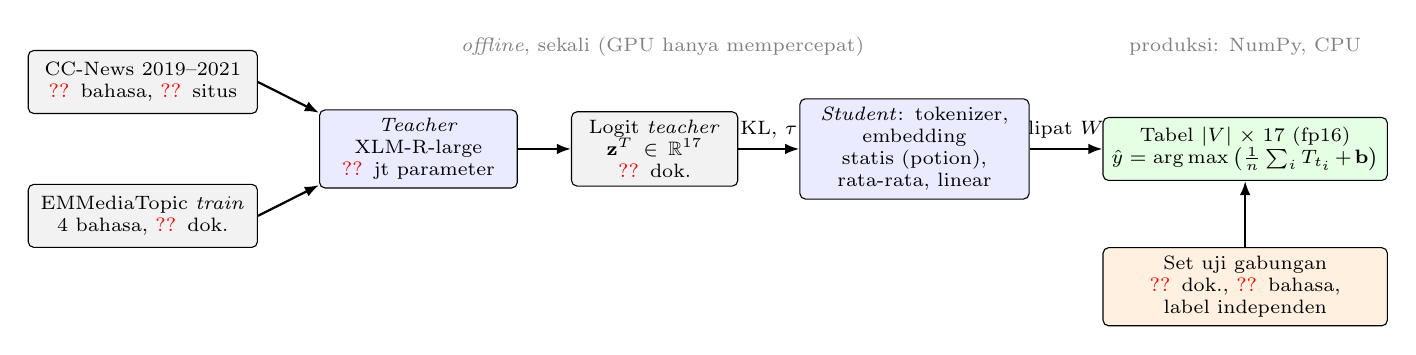
\begin{tikzpicture}[
  box/.style={draw, rounded corners=2pt, align=center, font=\scriptsize, inner sep=3pt, minimum height=8mm},
  data/.style={box, fill=gray!10},
  model/.style={box, fill=blue!8},
  prod/.style={box, fill=green!10},
  test/.style={box, fill=orange!12},
  arr/.style={-{Latex[length=1.8mm]}, thick},
  lab/.style={font=\scriptsize}]
  \node[data, text width=27mm] (cc)  at (1.4, 0.85)  {CC-News 2019--2021\\\val{data.pool.langs} bahasa, \val{data.pool.sites} situs};
  \node[data, text width=27mm] (emm) at (1.4,-0.85)  {EMMediaTopic \eng{train}\\4 bahasa, \val{emm.train} dok.};
  \node[model, text width=23mm] (t)  at (4.9, 0)     {\eng{Teacher}\\XLM-R-large\\\val{teacher.params} jt parameter};
  \node[data, text width=19mm] (soft) at (7.9, 0)    {Logit \eng{teacher}\\$\mathbf{z}^{T}\in\mathbb{R}^{17}$\\\val{data.pool.docs} dok.};
  \node[model, text width=27mm] (s)  at (11.2, 0)    {\eng{Student}: tokenizer,\\embedding statis (potion),\\rata-rata, linear};
  \node[prod, text width=34mm] (tab) at (15.4, 0)    {Tabel $|V|\times 17$ (fp16)\\$\hat{y}=\arg\max\big(\frac{1}{n}\sum_i T_{t_i}+\mathbf{b}\big)$};
  \node[test, text width=34mm] (ts) at (15.4, -1.75)  {Set uji gabungan\\\val{ts.docs} dok., \val{ts.langs} bahasa, label independen};
  \draw[arr] (cc.east)  -- (t.160);
  \draw[arr] (emm.east) -- (t.200);
  \draw[arr] (t) -- (soft);
  \draw[arr] (soft) -- node[lab, above]{KL, $\tau$} (s);
  \draw[arr] (s) -- node[lab, above]{lipat $W$} (tab);
  \draw[arr] (ts.north) -- (tab.south);
  \node[lab, text=gray] at (8.0, 1.3) {\eng{offline}, sekali (GPU hanya mempercepat)};
  \node[lab, text=gray] at (15.4, 1.3) {produksi: NumPy, CPU};
\end{tikzpicture}
\caption{Alur StaticKD. \eng{Teacher} melabeli korpus berita tak berlabel sekali secara \eng{offline}; \eng{student} dilatih meniru distribusi \eng{teacher}, lalu kepala linearnya dilipat ke dalam tabel token sehingga inferensi hanya berupa pengambilan baris tabel dan rata-rata. Evaluasi akhir memakai set uji yang labelnya independen dari \eng{teacher}.}
\label{fig:pipeline}
\end{figure*}

\subsection{Formulasi Masalah}
Diberikan artikel berita $d$ (judul dan isi, 512 kata pertama, sama dengan~\cite{kuzman2025llm}) dalam bahasa apa pun, model memprediksi satu label $y\in\mathcal{Y}$ dari 17 topik IPTC level atas. \eng{Teacher} $f_T$ menghasilkan logit $\mathbf{z}^T(d)\in\mathbb{R}^{17}$. Tujuannya adalah \eng{student} $f_S$ dengan biaya inferensi $O(n)$ operasi penjumlahan untuk $n$ token, tanpa perkalian matriks dan tanpa pustaka \eng{deep learning}, yang akurasinya terhadap label independen sedekat mungkin dengan $f_T$.

\subsection{Data Distilasi dan Set \eng{Development}}
\textbf{EMMediaTopic 1.0}~\cite{kuzman2025llm}\footnote{\url{http://hdl.handle.net/11356/1991}} berisi artikel berbahasa Katalan, Yunani, Kroasia, dan Slovenia yang dilabeli GPT-4o.
\begin{itemize}
  \item Split \eng{train} (\val{emm.train} artikel) dipakai sebagai data distilasi.
  \item Split \eng{dev} (\val{emm.dev} artikel, median \val{emm.dev.words} kata) tidak pernah dipakai melatih \eng{teacher} maupun \eng{student}. Split ini menjadi set \eng{development} untuk memilih resep.
\end{itemize}

\textbf{Korpus CC-News multibahasa}\footnote{\url{https://huggingface.co/datasets/CloverSearch/cc-news-mutlilingual}} diambil dari arsip 2019--2021 dengan aturan berikut.
\begin{enumerate}
  \item Hanya dokumen yang bahasa metadatanya sama dengan hasil fastText-LID.
  \item Teks berupa judul dan isi, minimal 75 kata (200 karakter untuk ja, zh, th, my), dipotong ke 512 kata.
  \item Maksimal 150 dokumen per situs.
  \item Split \eng{held-out} dibuat per domain: seluruh dokumen dari sebagian situs disisihkan, maksimal 20\% per bahasa.
  \item Sebanyak \val{data.ccextra.docs} dokumen tambahan (maksimal 5.000 per bahasa, maksimal 400 per situs) diambil hanya dari situs \eng{train}.
\end{enumerate}
Total data distilasi adalah \val{data.pool.docs} dokumen dari \val{data.pool.langs} bahasa (median \val{data.pool.words} kata).

Split \eng{held-out} bersifat \eng{domain-disjoint} di dalam setiap bahasa. Beberapa situs multibahasa (misalnya bbc.com) juga muncul di bahasa lain di data distilasi, sehingga artikelnya dikeluarkan. Set \eng{fidelity} akhirnya berisi \val{data.heldout.strict} dokumen dari \val{data.heldout.strict.langs} bahasa dan \val{data.heldout.strict.sites} situs yang tidak pernah muncul di data distilasi.

\subsection{Konstruksi Set Uji Gabungan}
\label{sec:testset}
\textbf{Sumber (a): CC-NEWS 2024--2026.} Satu file WARC per bulan, Januari 2024 sampai Agustus 2026 (32 file), diunduh dari arsip CC-NEWS Common Crawl\footnote{\url{https://data.commoncrawl.org/crawl-data/CC-NEWS/}}. Dari setiap halaman diambil blok JSON-LD schema.org\footnote{\url{https://schema.org/NewsArticle}} bertipe \texttt{NewsArticle} dan turunannya, beserta bidang \texttt{articleSection}, \texttt{BreadcrumbList}, \texttt{inLanguage}, \texttt{datePublished}, \texttt{isAccessibleForFree}, dan \texttt{articleBody}. Teks diambil dari \texttt{articleBody} bila berisi minimal 30 kata; jika tidak, teks diekstrak dengan Trafilatura\footnote{\url{https://github.com/adbar/trafilatura}}. Situs yang ada di data distilasi atau set evaluasi lain dikeluarkan. Hasilnya adalah \val{ts.html_articles} artikel dari situs baru.

\textbf{Sumber (b): dataset publik.}
\begin{itemize}
  \item Berlabel manusia: MasakhaNEWS~\cite{adelani2023masakhanews} dan MN-DS~\cite{petukhova2023mnds}.
  \item Berlabel kategori penerbit: L3Cube-IndicNews (split LDC)~\cite{mirashi2023indicnews}, berita Bangla~\cite{hossain2025banglanews}, IndoNews\footnote{\url{https://huggingface.co/datasets/jakartaresearch/indonews}}, berita Amharik\footnote{\url{https://huggingface.co/datasets/rasyosef/amharic-news-category-classification}}, dan berita Swahili\footnote{\url{https://doi.org/10.5281/zenodo.5514203}}. Dua sumber terakhir diproses dengan cara yang sama, tetapi tidak terpilih saat sampling karena sel bahasanya sudah terisi MasakhaNEWS yang berlabel manusia.
\end{itemize}
Totalnya \val{ts.ext_loaded} artikel.

\textbf{Pemetaan ke IPTC.} Nama rubrik atau kategori (setelah normalisasi huruf dan diakritik) dipetakan ke node pohon IPTC Media Topic resmi (\val{iptc.nodes} node aktif). Aturannya konservatif: sebuah nama hanya dipetakan bila \emph{seluruh isi yang lazim di rubrik itu} berada di bawah satu topik level atas. Hasilnya adalah \val{map.names} nama yang dipetakan ke \val{map.nodes} node. Sebanyak \val{map.ambiguous} nama ambigu sengaja tidak dipetakan, misalnya:
\begin{itemize}
  \item \eng{tech}: bisa \eng{science and technology} atau industri TI di \eng{economy};
  \item \eng{entertainment}: bisa \eng{arts} atau \eng{lifestyle};
  \item \eng{terrorism}: bisa \eng{conflict} atau \eng{crime}.
\end{itemize}
Rubrik astrologi ditolak. Validasi otomatis memeriksa bahwa setiap node tujuan ada di pohon IPTC, tidak berstatus \eng{retired}, dan leluhur level-1-nya sama dengan label tujuan. Artikel dengan beberapa rubrik yang dipetakan ke label berbeda ditolak. Label MN-DS dipakai langsung karena sudah berupa topik IPTC.

\textbf{Filter kualitas dan kebocoran.} Filter diterapkan berurutan.
\begin{enumerate}
  \item Tanggal terbit $\ge$ 2024-01-01 (khusus CC-NEWS).
  \item Artikel tidak berbayar.
  \item Bahasa yang dideklarasikan cocok dengan fastText lid.176 (bila bahasanya dikenal).
  \item Panjang $\ge$ 75 kata.
  \item Deduplikasi URL, teks identik, dan \eng{near-duplicate} (MinHash, Jaccard $\ge$ 0,7~\cite{lee2022dedup}) \emph{lintas semua sumber}.
  \item Kontaminasi: artikel dibuang bila $\ge$ 30\% 8-gram katanya muncul di salah satu dari $\sim$300 ribu dokumen latih atau evaluasi. Filter ini membuang \val{ts.contam_removed} artikel, sebagian besar dari MasakhaNEWS yang juga bersumber dari BBC.
\end{enumerate}

\textbf{Sampling.}
\begin{itemize}
  \item Maksimal 50 artikel per sel (bahasa $\times$ label).
  \item Sumber berlabel manusia diprioritaskan, lalu kategori penerbit, lalu rubrik JSON-LD.
  \item Bahasa dengan kurang dari 30 artikel dikeluarkan.
  \item Tidak ada batas jumlah artikel per situs. Kebanyakan sel hanya berasal dari sedikit situs, sehingga batas seperti itu membuang data tanpa menambah keragaman. Ketergantungan antarartikel dari situs yang sama ditangani saat evaluasi dengan \eng{site-cluster bootstrap}, dan Subbagian~\ref{sec:res-acc} menyertakan uji sensitivitas dengan batas 5 artikel per situs.
\end{itemize}

\textbf{Hasil.} Set uji berisi \val{ts.docs} artikel dari \val{ts.langs} bahasa, \val{ts.labels} label, dan \val{ts.sites} situs atau sumber (median \val{ts.words} kata), dengan komposisi asal label:
\begin{itemize}
  \item anotasi manusia: \val{ts.origin.human_annotation} artikel (\val{ts.origin.human_annotation.pct});
  \item kategori penerbit: \val{ts.origin.publisher_category} artikel (\val{ts.origin.publisher_category.pct});
  \item rubrik JSON-LD: \val{ts.origin.publisher_section_jsonld} artikel (\val{ts.origin.publisher_section_jsonld.pct}).
\end{itemize}
Menurut data distilasi di bahasanya, \val{ts.distil.tidak.langs} bahasa sama sekali tidak ada di data distilasi (misalnya ha, yo, ig, bn, pa), \val{ts.distil.sedikit.langs} bahasa punya kurang dari 500 dokumen, dan \val{ts.distil.cukup.langs} bahasa punya sisanya. Menurut keragaman situs, \val{ts.div.beragam.langs} bahasa memiliki minimal 10 situs efektif, sedangkan \val{ts.div.satu.langs} bahasa praktis berasal dari satu penerbit. Tabel~\ref{tab:testset} merangkum sumber dan Gbr.~\ref{fig:testset} memperlihatkan cakupan bahasa $\times$ label.

\begin{table}[!t]
\caption{Komposisi Set Uji Gabungan per Sumber}
\label{tab:testset}
\centering
\footnotesize
\setlength{\tabcolsep}{3pt}
\resizebox{\columnwidth}{!}{%
\begin{tabular}{@{}llrrr@{}}
\toprule
Sumber & Asal label & Artikel & Bahasa & Situs/sumber \\
\midrule
\rows{generated/tab_testset}
\bottomrule
\end{tabular}}
\end{table}

\begin{figure}[!t]
\centering
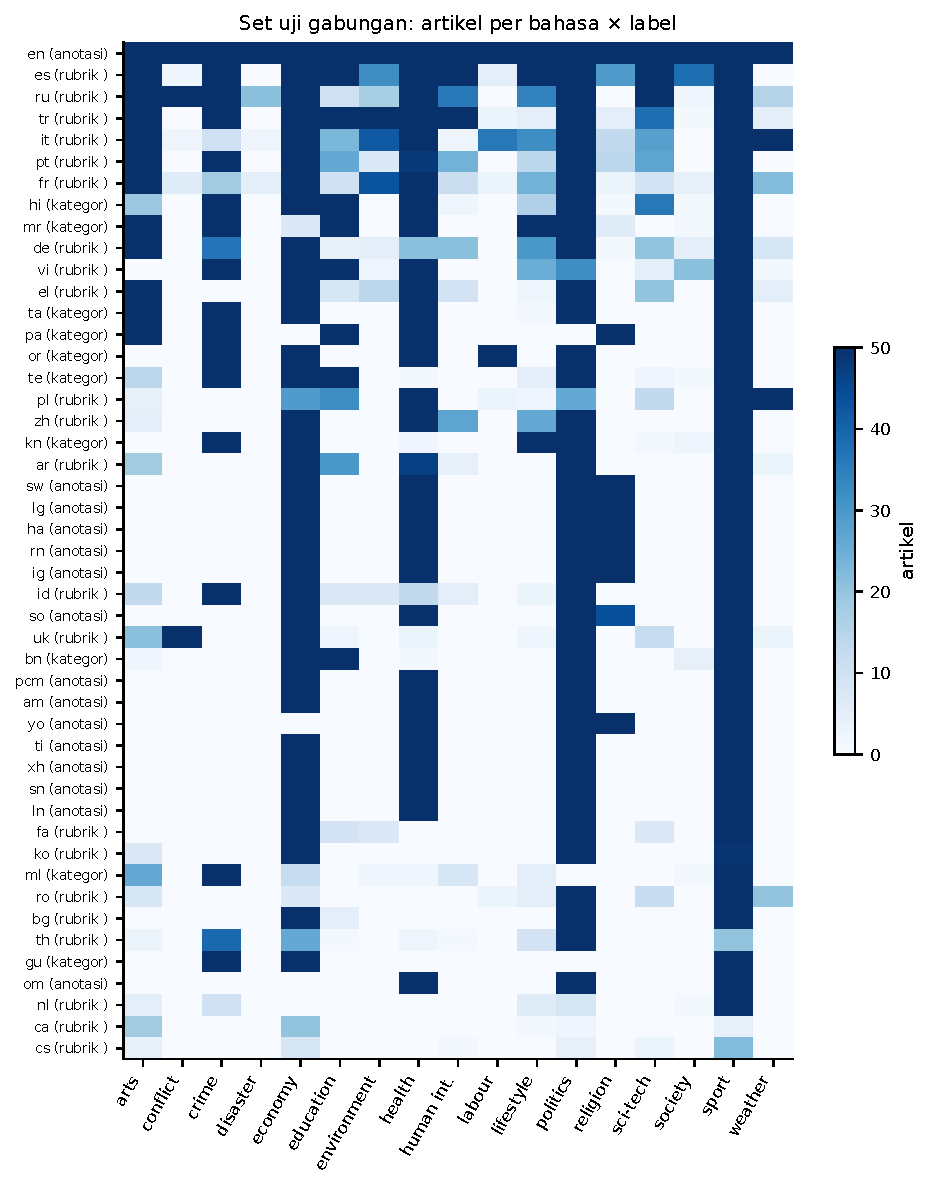
\includegraphics[width=\columnwidth]{figures/fig_testset_heatmap.pdf}
\caption{Jumlah artikel set uji gabungan per bahasa dan label (maksimal 50 per sel). Label dalam kurung adalah asal label dominan bahasa tersebut.}
\label{fig:testset}
\end{figure}

\subsection{\eng{Teacher} dan Pelabelan Distilasi}
\eng{Teacher} adalah \url{classla/multilingual-IPTC-news-topic-classifier}~\cite{kuzman2025llm}: XLM-RoBERTa-large dengan \val{teacher.layers} \eng{layer}, \val{teacher.params} juta parameter, dan maksimal 512 token. Untuk setiap dokumen distilasi, \eng{teacher} menghasilkan vektor logit $\mathbf{z}^{T}(d)\in\mathbb{R}^{17}$ yang disimpan utuh. Pelabelan dijalankan sekali dalam fp16 pada GPU RTX~4050, dengan \eng{batch} yang diurutkan berdasarkan panjang teks. Distribusi label \eng{teacher} pada CC-News wajar (\eng{politics} \val{teacher.share.politics}, \eng{economy} \val{teacher.share.economy}, \eng{sport} \val{teacher.share.sport}, \eng{weather} \val{teacher.share.weather}), dan keyakinan rata-ratanya per bahasa berkisar \val{teacher.conf.min}--\val{teacher.conf.max}.

\subsection{\eng{Student} StaticKD}
\textbf{Arsitektur.} Dokumen $d$ ditokenisasi menjadi $t_1,\dots,t_n$ dengan tokenizer Unigram \eng{potion-multilingual-128M}~\cite{tulkens2024model2vec} (\val{student.vocab} token; tanpa token khusus; token tidak dikenal dibuang; maksimal 1.024 token). Setiap token memiliki embedding $\mathbf{e}_t\in\mathbb{R}^{\val{student.dim}}$, dan
\begin{equation}
\mathbf{h}(d)=\frac{1}{n}\sum_{i=1}^{n}\mathbf{e}_{t_i},\qquad
\mathbf{z}^{S}(d)=W\,\mathrm{drop}(\mathbf{h}(d))+\mathbf{b},
\label{eq:student}
\end{equation}
dengan $W\in\mathbb{R}^{17\times 256}$ dan \eng{dropout} 0,1 selama \eng{training}. Matriks $E$ diinisialisasi dari potion-multilingual, yaitu embedding statis 101 bahasa yang didistilasi dari BGE-M3~\cite{chen2024bgem3}.

\textbf{Fungsi \eng{loss}.} Dengan $p^{T}=\mathrm{softmax}(\mathbf{z}^{T}/\tau)$ dan $p^{S}=\mathrm{softmax}(\mathbf{z}^{S}/\tau)$,
\begin{equation}
\mathcal{L}_{\mathrm{KD}}=\tau^{2}\,\mathrm{KL}\!\left(p^{T}\,\middle\|\,p^{S}\right),\qquad \tau=1 .
\label{eq:kd}
\end{equation}

\textbf{Optimasi.} $E$, $W$, dan $\mathbf{b}$ dilatih \eng{end-to-end}.
\begin{itemize}
  \item $E$ memakai SparseAdam ($\eta=10^{-3}$), sehingga hanya baris token yang muncul di \eng{batch} yang diperbarui.
  \item $W$ dan $\mathbf{b}$ memakai AdamW ($\eta=3\cdot 10^{-3}$, \eng{weight decay} $10^{-4}$).
  \item Ukuran \eng{batch} 64 dan 6 \eng{epoch}.
  \item \eng{Token dropout}: setiap token dokumen latih dibuang dengan probabilitas 0,2 pada setiap langkah, sebagai augmentasi murah agar model tidak bergantung pada beberapa kata kunci.
  \item Sebanyak 3\% data distilasi (\val{train.val_docs} dokumen) disisihkan sebagai validasi internal. \eng{Epoch} dengan kesepakatan \eng{argmax} tertinggi terhadap \eng{teacher} dipilih.
\end{itemize}

\textbf{Pelipatan tabel.} Karena kepala klasifikasinya linear,
\begin{equation}
W\Big(\frac{1}{n}\sum_{i}\mathbf{e}_{t_i}\Big)+\mathbf{b}=\frac{1}{n}\sum_{i}T_{t_i}+\mathbf{b},\qquad T=EW^{\top}\in\mathbb{R}^{|V|\times 17}.
\label{eq:fold}
\end{equation}
Model produksi hanyalah $T$ (fp16), $\mathbf{b}$, dan tokenizer. Inferensi terdiri atas tokenisasi, rata-rata baris tabel, dan penambahan bias.

\textbf{\eng{Ensemble} tanpa biaya.} Rata-rata logit $K$ \eng{student} dengan \eng{seed} berbeda sama dengan logit satu \eng{student} bertabel $\bar{T}=\frac{1}{K}\sum_k T^{(k)}$ dan bias $\bar{\mathbf{b}}$ (Persamaan~\ref{eq:fold} linear terhadap $T$). StaticKD final adalah \eng{ensemble} tabel \eng{seed} 0, 1, dan 2 ($K=3$), dengan \val{final.params} juta parameter dan ukuran \val{final.size}~MB.

\textbf{Varian \eng{compact}.} Struktur internal tokenizer Unigram membutuhkan RAM jauh lebih besar daripada tabelnya (\val{final.table_mb}~MB). Varian \eng{compact} membuang potongan token yang muncul kurang dari 10 kali di korpus distilasi (karakter tunggal dipertahankan), sehingga kosakata menjadi \val{compact.vocab} token dan ukuran model \val{compact.size}~MB.

\begin{table}[!t]
\caption{Hiperparameter Seluruh Model}
\label{tab:hparams}
\centering
\footnotesize
\setlength{\tabcolsep}{3pt}
\resizebox{\columnwidth}{!}{%
\begin{tabular}{@{}ll@{}}
\toprule
Komponen & Nilai \\
\midrule
\rows{generated/tab_hparams}
\bottomrule
\end{tabular}}
\end{table}

\subsection{\eng{Baseline}}
Semua \eng{baseline} dilatih pada data distilasi yang sama (\val{data.pool.docs} dokumen) dengan target \eng{teacher} yang sama. Hiperparameternya ada di Tabel~\ref{tab:hparams}.
\begin{enumerate}
  \item \textbf{fastText + KD}~\cite{joulin2017bag}: dilatih dengan \eng{argmax} \eng{teacher}, memakai token kata (dengan n-gram karakter) atau subword XLM-R, ditambah varian terkuantisasi (\texttt{.ftz}).
  \item \textbf{fastText, label GPT-4o}: dilatih hanya pada EMMediaTopic \eng{train}, sama dengan data berlabel yang tersedia bagi~\cite{kuzman2025llm}.
  \item \textbf{TF-IDF + SVM + KD}: \eng{baseline} non-neural Kuzman dan Ljube\v{s}i\'c (TF-IDF + SVC), dilatih dengan \eng{argmax} \eng{teacher} di atas subword XLM-R.
  \item \textbf{MiniLM-L6 + KD}: mMiniLMv2-L6-H384 yang didistilasi dari XLM-R-large~\cite{wang2021minilmv2}. \eng{Temperature} $\tau\in\{1,2\}$ dipilih pada set \eng{development}.
  \item \textbf{DistilmBERT + KD}: \url{distilbert-base-multilingual-cased} dengan resep yang sama. Kedua transformer diekspor ke ONNX fp32 untuk \eng{benchmark} CPU.
  \item \textbf{\eng{Teacher} ONNX int8}: ekspor kuantisasi \eng{dynamic} int8 dari \eng{teacher}, konfigurasi CPU tercepat untuk \eng{teacher}.
\end{enumerate}

\subsection{Protokol Evaluasi dan Uji Statistik}
\label{sec:protocol}
\textbf{Metrik.}
\begin{itemize}
  \item Macro-F1 atas label yang hadir di referensi, sama dengan kode evaluasi~\cite{kuzman2025llm}. Ini metrik utama karena distribusi labelnya tidak seimbang.
  \item Akurasi.
  \item Macro-F1 per bahasa yang dirata-rata antarbahasa, supaya bahasa besar tidak mendominasi.
  \item Kesepakatan dengan \eng{teacher} pada set \eng{fidelity}.
\end{itemize}

\textbf{Interval kepercayaan} 95\% dihitung dengan \eng{bootstrap percentile} 1.000 kali. Di set uji yang di-\eng{resample} adalah situs (atau dataset sumber bila tidak ada URL), yaitu \eng{site-cluster bootstrap}~\cite{field2007bootstrapping}. Di dev yang di-\eng{resample} adalah dokumen.

\textbf{Perbandingan dua model} pada dokumen yang sama:
\begin{itemize}
  \item \eng{paired (cluster) bootstrap} 2.000 kali untuk $\Delta$macro-F1~\cite{koehn2004significance};
  \item uji McNemar eksak untuk akurasi;
  \item koreksi Holm--Bonferroni per set.
\end{itemize}

\textbf{Variasi antar-\eng{seed}.} Setiap varian ablasi dilatih dengan lima \eng{seed} dan resep final dengan sepuluh \eng{seed}. Perbedaannya diuji dengan uji Welch pada tingkat \eng{seed}, dikoreksi Holm.

\textbf{Analisis subkelompok} dilakukan menurut asal label, wilayah, jumlah data distilasi bahasa, keragaman situs, sistem tulisan, bahasa, dan label.

\textbf{Kalibrasi} diukur dengan \eng{expected calibration error} (ECE, 15 \eng{bin}).

\subsection{Protokol Efisiensi}
\label{sec:effprotocol}
\eng{Benchmark} dijalankan hanya di CPU, dengan GPU disembunyikan.
\begin{itemize}
  \item Setiap model dijalankan di proses baru, dan jumlah \eng{thread} dikunci pada seluruh pustaka (OMP, MKL, OpenBLAS, ONNX Runtime, \texttt{tokenizers}).
  \item Latensi diukur dengan satu artikel per panggilan (skenario \eng{streaming}; p50 dan p95).
  \item \eng{Throughput} diukur dengan \eng{batch} 64, atau 8 untuk transformer.
  \item RAM model adalah kenaikan RSS setelah model dimuat.
  \item Sampel teks adalah sampel acak tetap dari set uji gabungan (\val{ts.langs} bahasa), sama untuk semua model.
  \item Perangkat: Intel Core Ultra~7 155H, RAM 31~GB, Windows~11.
\end{itemize}
CPU ini bersifat \eng{hybrid}: 6 P-\eng{core}, 8 E-\eng{core} yang sekitar 2,5 kali lebih lambat, dan 2 LP E-\eng{core}. Tanpa \eng{pinning}, sistem operasi memindahkan \eng{thread} ke \eng{core} lambat. Karena itu setiap proses dipin ke P-\eng{core} fisik (1 \eng{core}: CPU logis 0; 4 \eng{core}: CPU logis 0, 10, 12, 14) untuk mensimulasikan server kecil dengan \eng{core} seragam. Semua model diukur dalam satu sesi saat mesin idle.

\subsection{Desain Eksperimen dan Detail Implementasi}
Tabel~\ref{tab:ablation} mendaftar seluruh \val{runs.total} run StaticKD. Setiap varian mengubah satu faktor terhadap resep final:
\begin{itemize}
  \item label keras;
  \item data EMMediaTopic saja (4 bahasa, 10 \eng{epoch});
  \item 130 ribu dokumen tanpa CC-News tambahan;
  \item inisialisasi acak dengan simpangan baku yang sama dengan potion;
  \item embedding beku;
  \item tanpa \eng{token dropout};
  \item kepala MLP 512 unit;
  \item $\tau\in\{0{,}5; 2; 4\}$;
  \item empat varian eksplorasi (bigram \eng{hashing} $2^{21}$, \eng{pooling} berbobot idf$^{0,5}$, bobot dokumen berdasarkan keyakinan \eng{teacher}, dan \eng{cross-entropy} tambahan terhadap label GPT-4o).
\end{itemize}
Satu run StaticKD rata-rata membutuhkan \val{train.seconds} menit pada RTX~4050. Implementasi memakai Python~3.12, PyTorch~2.6, \texttt{tokenizers}~0.23, ONNX Runtime~1.30, scikit-learn~1.9, dan fastText~0.9.2. \eng{Seed}, versi pustaka, dan riwayat \eng{training} setiap run disimpan bersama model.

% =====================================================================
\section{Hasil}
\label{sec:results}
\subsection{Akurasi Seluruh Model (RQ2)}
\label{sec:res-acc}
\TabMain
Tabel~\ref{tab:main} memuat hasil utama.

\textbf{Set uji gabungan.}
\begin{itemize}
  \item \eng{Teacher} mencapai macro-F1 \val{teacher.test.macro} [\val{teacher.test.ci}] dan akurasi \val{teacher.test.acc}. Angka ini jauh di bawah skornya di dev (\val{teacher.dev.macro}), karena set uji mencakup bahasa, sumber, dan periode yang tidak pernah dilihat.
  \item StaticKD mencapai macro-F1 \val{statickd.test.macro} [\val{statickd.test.ci}] dan akurasi \val{statickd.test.acc}, atau \val{statickd.test.pct_teacher} dari macro-F1 \eng{teacher}.
  \item Pada dev, StaticKD mempertahankan \val{statickd.dev.pct_teacher} macro-F1 \eng{teacher} (\val{statickd.dev.macro} vs \val{teacher.dev.macro}).
  \item Kesepakatan StaticKD dengan \eng{teacher} di \val{data.heldout.strict.langs} bahasa \eng{held-out} adalah \val{statickd.heldout.acc}.
  \item Satu \eng{student} tanpa \eng{ensemble} mencapai rata-rata \val{single.test_macro.mean} $\pm$ \val{single.test_macro.sd} (10 \eng{seed}) di set uji dan \val{single.dev_macro.mean} $\pm$ \val{single.dev_macro.sd} di dev.
\end{itemize}

\textbf{\eng{Baseline}.}
\begin{itemize}
  \item Di antara transformer kecil hasil distilasi, MiniLM-L6 (\val{minilm_kd.test.macro}), yang diinisialisasi dari distilasi XLM-R-large, berada di antara StaticKD dan \eng{teacher}. DistilmBERT (\val{distilmbert_kd.test.macro}) justru berada di bawah StaticKD walaupun jauh lebih mahal.
  \item \eng{Baseline} berbiaya serupa (fastText + KD, TF-IDF + SVM + KD) berada di bawah StaticKD.
  \item fastText yang hanya dilatih dengan label GPT-4o empat bahasa gagal di luar bahasa latihnya (macro-F1 uji \val{ft_gpt_subword.test.macro}), walaupun cukup baik di dev (\val{ft_gpt_subword.dev.macro}).
\end{itemize}

\TabSig
\textbf{Uji berpasangan} (Tabel~\ref{tab:sig}), dengan $\Delta$ = StaticKD $-$ pembanding pada set uji:
\begin{itemize}
  \item terhadap \eng{teacher}: $\Delta$macro-F1 \val{sig.test.teacher.delta} [\val{sig.test.teacher.ci}], $p$ \val{sig.test.teacher.p};
  \item terhadap MiniLM-L6: \val{sig.test.minilm_kd.delta} [\val{sig.test.minilm_kd.ci}], $p$ \val{sig.test.minilm_kd.p};
  \item terhadap DistilmBERT: \val{sig.test.distilmbert_kd.delta} [\val{sig.test.distilmbert_kd.ci}], $p$ \val{sig.test.distilmbert_kd.p};
  \item terhadap fastText + KD terkuantisasi: \val{sig.test.ft_kd_subword_q.delta} [\val{sig.test.ft_kd_subword_q.ci}], $p$ \val{sig.test.ft_kd_subword_q.p};
  \item terhadap TF-IDF + SVM: \val{sig.test.tfidf_svm_kd.delta} [\val{sig.test.tfidf_svm_kd.ci}], $p$ \val{sig.test.tfidf_svm_kd.p}.
\end{itemize}

\textbf{Menurut subkelompok} (Tabel~\ref{tab:groups}, Gbr.~\ref{fig:groups}):
\begin{itemize}
  \item Pada artikel berlabel rubrik JSON-LD, StaticKD mempertahankan \val{grp.label_origin.publishersection.pct} skor \eng{teacher}.
  \item Pada kategori penerbit angkanya \val{grp.label_origin.publishercategor.pct}, dan pada anotasi manusia \val{grp.label_origin.humanannotation.pct}.
  \item Menurut data distilasi bahasa, StaticKD mempertahankan \val{grp.distil_tier.cukup.pct} skor \eng{teacher} di bahasa dengan data cukup, \val{grp.distil_tier.sedikit.pct} di bahasa dengan sedikit data, dan \val{grp.distil_tier.tidakada.pct} di bahasa yang sama sekali tidak ada di data distilasi.
\end{itemize}

\textbf{Uji sensitivitas} pada subset dengan maksimal lima artikel per situs per sel (\val{sens.n} artikel) menghasilkan peringkat model yang \val{sens.rank_same} dengan set uji penuh (StaticKD \val{sens.statickd}, \eng{teacher} \val{sens.teacher}).

\TabGroups

\begin{figure*}[!t]
\centering
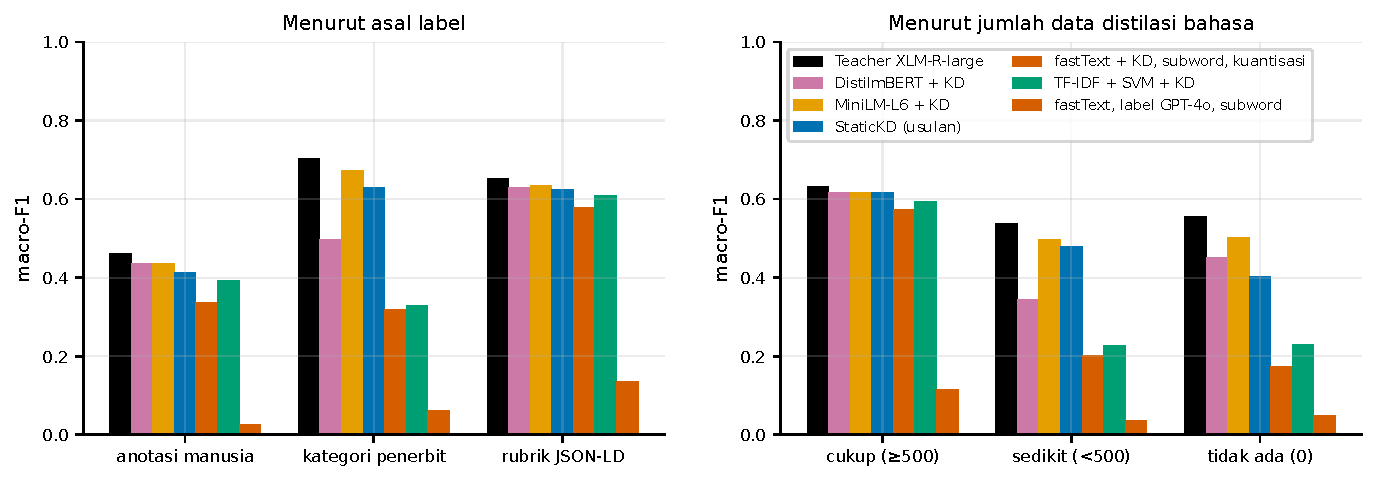
\includegraphics[width=0.9\textwidth]{figures/fig_groups.pdf}
\caption{Macro-F1 set uji menurut asal label (kiri) dan menurut jumlah data distilasi di bahasa artikel (kanan).}
\label{fig:groups}
\end{figure*}

\subsection{Validitas Label Silver}
\label{sec:res-validity}
Label silver diperiksa secara tidak langsung dengan dua cara.
\begin{enumerate}
  \item \textbf{Perbandingan dengan label manusia di bahasa yang sama.} Seluruh sel bahasa Inggris di set uji terisi sumber berlabel manusia. Karena itu diambil sampel terpisah berisi \val{valid.en.silver.n} artikel CC-NEWS berbahasa Inggris berlabel rubrik JSON-LD dari \val{valid.en.silver.sites} situs yang tidak masuk set uji, maksimal 50 per label.
  \begin{itemize}
    \item Akurasi \eng{teacher} pada label silver adalah \val{valid.en.silver.acc} (macro-F1 \val{valid.en.silver.macro}), sedangkan pada label manusia MN-DS/MasakhaNEWS \val{valid.en.human.acc} (macro-F1 \val{valid.en.human.macro}).
    \item Akurasinya lebih tinggi pada label silver di \val{valid.en.labels_higher} dari 17 label (Wilcoxon $p$ \val{valid.en.wilcoxon.p}).
    \item Urutan tingkat kesulitan label pada kedua jenis label berkorelasi ($\rho=\val{valid.en.label_rho}$, $p$ \val{valid.en.label_rho.p}).
  \end{itemize}
  Dengan kata lain, label silver tidak lebih bising daripada label manusia yang tersedia, setidaknya jika diukur dengan kesepakatan terhadap \eng{teacher}. Label yang sulit (\eng{society}, \eng{human interest}, \eng{religion}) sulit di kedua jenis label.
  \item \textbf{Pemeriksaan per kategori sumber}, hanya pada bahasa yang tercakup pra-latih XLM-R. Median kesepakatan \eng{teacher} dengan label hasil pemetaan per kategori adalah \val{mapcheck.masakhanews.median} untuk MasakhaNEWS, \val{mapcheck.mnds.median} untuk MN-DS, \val{mapcheck.l3cube_indic.median} untuk L3Cube, dan \val{mapcheck.ccnews_jsonld.median} untuk rubrik CC-NEWS. Kesepakatan terendah muncul pada dua jenis kategori.
  \begin{itemize}
    \item Kategori sumber yang cakupannya lebih luas daripada topik IPTC tujuannya. Contohnya, MasakhaNEWS \eng{politics} hanya \val{mapcheck.masakha_politics} sesuai, dengan alternatif utama \val{mapcheck.masakha_politics.alt}.
    \item Label yang batasnya kabur bahkan bagi anotator manusia, misalnya MN-DS \eng{society}, sejalan dengan kesepakatan antaranotator yang rendah pada label tersebut~\cite{kuzman2025llm}.
  \end{itemize}
\end{enumerate}
Karena itu, skor absolut pada label berskema non-IPTC merupakan batas bawah akurasi yang sebenarnya, sedangkan perbandingan antarmodel tetap sahih karena semua model dinilai terhadap label yang sama.

\subsection{Ablasi, \eng{Temperature}, dan \eng{Ensemble} (RQ3)}
\TabAblation
\TabAblationGroups
Tabel~\ref{tab:ablation} merangkum kontribusi setiap komponen, dengan lima \eng{seed} per varian.
\begin{itemize}
  \item \textbf{Data distilasi multibahasa adalah komponen terpenting.} Distilasi hanya pada EMMediaTopic (4 bahasa) menurunkan macro-F1 uji sebesar \val{abl.emm_only.test_macro.delta} dan kesepakatan \eng{held-out} sebesar \val{abl.emm_only.heldout_acc.delta}.
  \item \textbf{Inisialisasi embedding yang selaras lintas bahasa.} Inisialisasi acak mengubah macro-F1 uji sebesar \val{abl.random_init.test_macro.delta} ($p$ \val{abl.random_init.test_macro.p}).
  \item \textbf{\eng{Fine-tuning} embedding: kecocokan in-distribusi vs transfer.} Membekukan embedding potion dan hanya melatih kepala linear menurunkan dev sebesar \val{abl.frozen.dev_macro.delta} ($p$ \val{abl.frozen.dev_macro.p}) dan kesepakatan \eng{held-out} sebesar \val{abl.frozen.heldout_acc.delta} ($p$ \val{abl.frozen.heldout_acc.p}), tetapi \emph{menaikkan} macro-F1 uji sebesar \val{abl.frozen.test_macro.delta} ($p$ \val{abl.frozen.test_macro.p}). Tabel~\ref{tab:ablation-groups} menunjukkan bahwa kenaikan ini seluruhnya berasal dari bahasa dengan sedikit data distilasi (\val{ablgrp.frozen.sedikit.delta}) dan tanpa data distilasi (\val{ablgrp.frozen.tidakada.delta}), sedangkan di bahasa kaya data embedding beku lebih lemah (\val{ablgrp.frozen.cukup.delta}).
  \item \textbf{\eng{Soft label}.} Label keras \eng{teacher} mengubah macro-F1 uji sebesar \val{abl.hard.test_macro.delta} ($p$ \val{abl.hard.test_macro.p}) dan dev sebesar \val{abl.hard.dev_macro.delta} ($p$ \val{abl.hard.dev_macro.p}).
  \item \textbf{Ukuran data.} Mengurangi data ke 130 ribu dokumen mengubah macro-F1 uji sebesar \val{abl.data130k.test_macro.delta} ($p$ \val{abl.data130k.test_macro.p}).
  \item \textbf{\eng{Token dropout}.} Tanpa \eng{token dropout}, macro-F1 uji berubah sebesar \val{abl.no_tdrop.test_macro.delta} ($p$ \val{abl.no_tdrop.test_macro.p}).
  \item \textbf{Kepala MLP.} Kepala MLP, yang tidak dapat dilipat, mengubah macro-F1 uji sebesar \val{abl.mlp.test_macro.delta} ($p$ \val{abl.mlp.test_macro.p}).
\end{itemize}

\textbf{\eng{Temperature}} (Gbr.~\ref{fig:temperature}). Dibanding $\tau=1$:
\begin{itemize}
  \item $\tau=2$, nilai yang lazim dipakai~\cite{hinton2015distilling}, mengubah dev sebesar \val{abl.tau2.dev_macro.delta} ($p$ \val{abl.tau2.dev_macro.p}) dan kesepakatan \eng{held-out} sebesar \val{abl.tau2.heldout_acc.delta} ($p$ \val{abl.tau2.heldout_acc.p});
  \item $\tau=4$ mengubah macro-F1 uji sebesar \val{abl.tau4.test_macro.delta} ($p$ \val{abl.tau4.test_macro.p}).
\end{itemize}

\textbf{Varian eksplorasi} (bigram \eng{hashing}, \eng{pooling} idf, bobot keyakinan, label GPT-4o) tidak memperbaiki set uji. Hasilnya: bigram \val{abl.bigram.test_macro.delta}, idf \val{abl.idf.test_macro.delta}, bobot keyakinan \val{abl.conf.test_macro.delta}, dan CE GPT-4o \val{abl.gpt_ce.test_macro.delta}.

\textbf{\eng{Ensemble}} (Gbr.~\ref{fig:ensemble}). Menaikkan ukuran \eng{ensemble} dari satu ke tiga \eng{seed} mengubah macro-F1 uji rata-rata dari \val{ens.k1.test_macro} menjadi \val{ens.k3.test_macro}, dan kesepakatan \eng{held-out} dari \val{ens.k1.heldout_acc} menjadi \val{ens.k3.heldout_acc}. Sepuluh \eng{seed} memberi \val{ens.k10.test_macro}. Semua ukuran \eng{ensemble} tetap berupa satu tabel dengan biaya inferensi yang sama.

\begin{figure*}[!t]
\centering
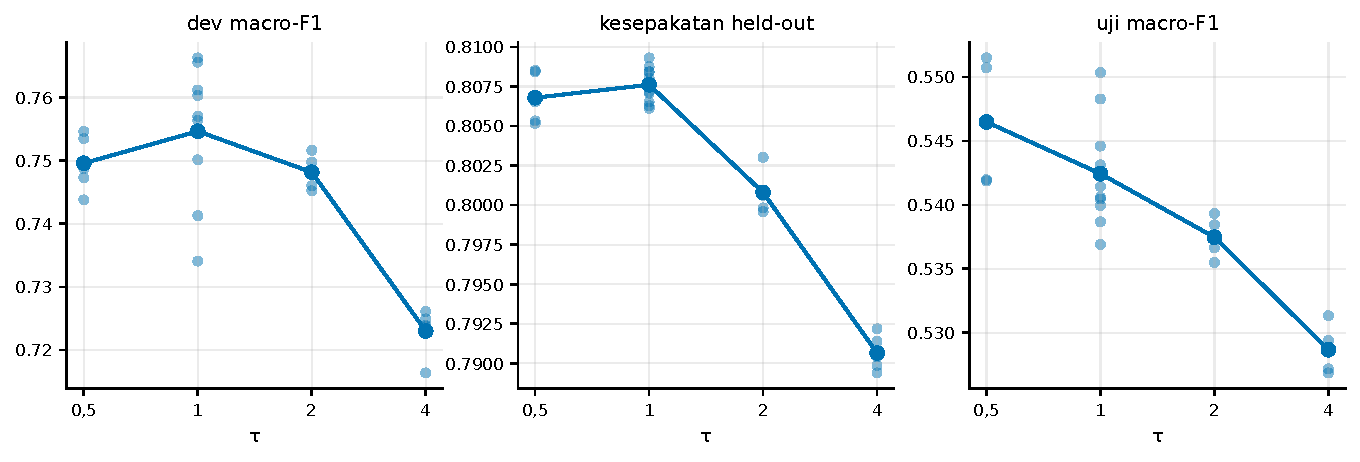
\includegraphics[width=0.9\textwidth]{figures/fig_temperature.pdf}
\caption{Pengaruh \eng{temperature} distilasi. Titik = satu \eng{seed}, garis = rata-rata.}
\label{fig:temperature}
\end{figure*}

\begin{figure}[!t]
\centering
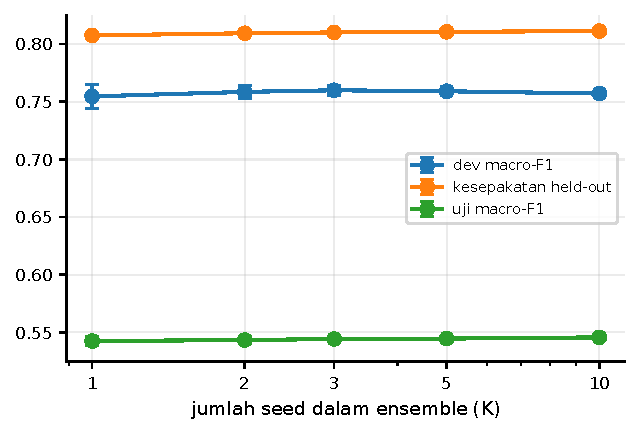
\includegraphics[width=0.85\columnwidth]{figures/fig_ensemble_size.pdf}
\caption{Pengaruh ukuran \eng{ensemble} tabel (rata-rata $\pm$ SD atas kombinasi \eng{seed}).}
\label{fig:ensemble}
\end{figure}

\subsection{Efisiensi CPU (RQ1)}
\label{sec:res-eff}
\TabEff
Tabel~\ref{tab:eff} dan Gbr.~\ref{fig:tradeoff}--\ref{fig:latency} menunjukkan efisiensi seluruh model.

\textbf{\eng{Teacher}.} Dalam PyTorch fp32, \eng{teacher} membutuhkan \val{eff.teacher.latency_ms_p50_1c}~ms per artikel pada satu \eng{core}, dengan \eng{throughput} \val{eff.teacher.docs_per_sec_1c} artikel per detik. Konfigurasi CPU terbaiknya, ONNX int8, membutuhkan \val{eff.teacher_onnx_int8.latency_ms_p50_1c}~ms dengan \eng{throughput} \val{eff.teacher_onnx_int8.docs_per_sec_1c} artikel per detik. Untuk satu juta artikel per hari dibutuhkan \val{eff.teacher_onnx_int8.cores1M} \eng{core} (ONNX int8) sampai \val{eff.teacher.cores1M} \eng{core} (PyTorch) khusus untuk klasifikasi.

\textbf{StaticKD.}
\begin{itemize}
  \item Latensi \val{eff.statickd.latency_ms_p50_1c}~ms dan \eng{throughput} \val{eff.statickd.docs_per_sec_1c} artikel per detik per \eng{core}.
  \item Sekitar \val{eff.statickd.speedup_onnx} kali lebih cepat dari \eng{teacher} ONNX int8, \val{eff.statickd.speedup_pt} kali lebih cepat dari \eng{teacher} PyTorch, dan \val{eff.speed_vs_minilm} kali lebih cepat dari MiniLM-L6.
  \item Ukuran file \val{eff.size_ratio_onnx} kali lebih kecil dari \eng{teacher} ONNX int8.
  \item Satu juta artikel per hari hanya membutuhkan \val{eff.statickd.cores1M} \eng{core}.
  \item RAM model \val{eff.statickd.ram}~MB, sebagian besar dipakai struktur tokenizer. Varian \eng{compact} menurunkannya ke \val{eff.statickd_compact.ram}~MB.
  \item \textbf{Tokenisasi adalah hampir seluruh biaya.} Pada satu \eng{thread}, tokenisasi (rata-rata \val{prof.statickd.tokens} token per artikel) memakan \val{prof.statickd.tokshare} waktu prediksi. \eng{Pooling} tabel sendiri berjalan pada \val{prof.statickd.pool_dps} artikel per detik. Batas kecepatan StaticKD karena itu ditentukan oleh implementasi tokenizer, bukan oleh model.
\end{itemize}

\begin{figure}[!t]
\centering
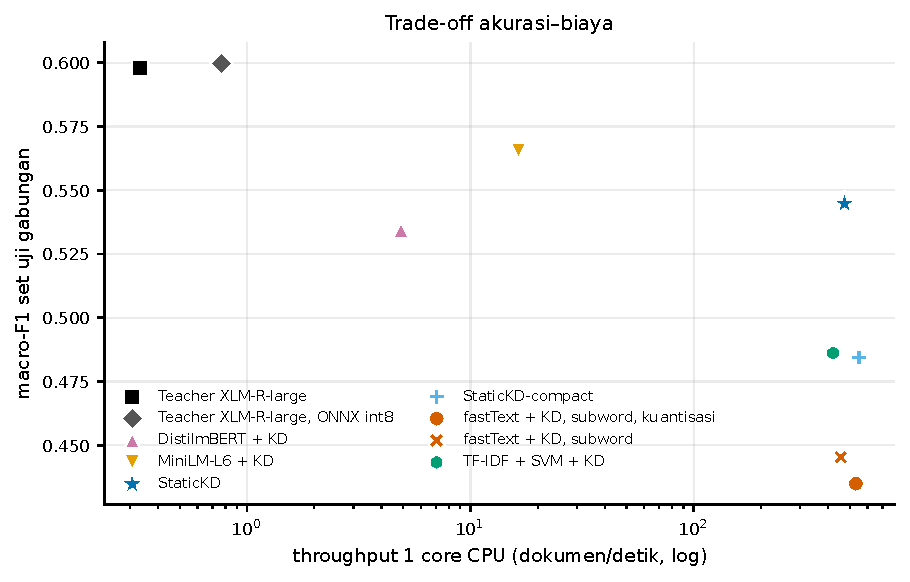
\includegraphics[width=\columnwidth]{figures/fig_tradeoff.pdf}
\caption{\eng{Trade-off} macro-F1 set uji gabungan terhadap \eng{throughput} satu \eng{core} CPU (skala log).}
\label{fig:tradeoff}
\end{figure}

\begin{figure*}[!t]
\centering
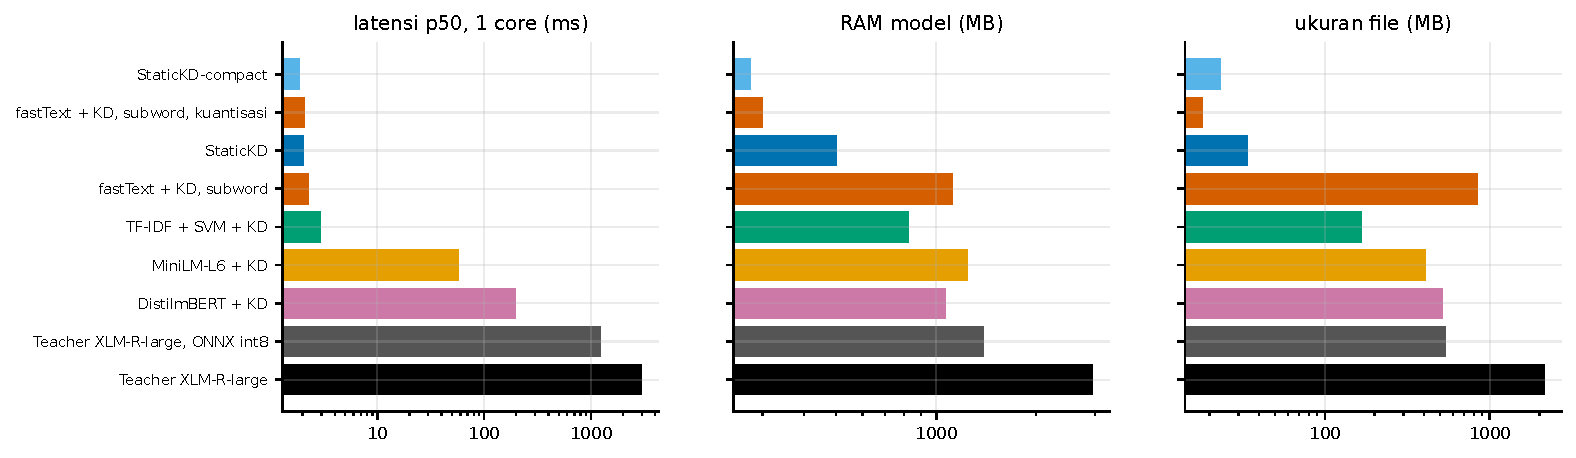
\includegraphics[width=0.9\textwidth]{figures/fig_latency_ram_size.pdf}
\caption{Latensi per artikel, RAM model, dan ukuran file (skala log).}
\label{fig:latency}
\end{figure*}

\subsection{Analisis per Bahasa dan per Label (RQ4)}
\TabFactors

\textbf{Per bahasa} (Gbr.~\ref{fig:lang}).
\begin{itemize}
  \item Median selisih akurasi StaticKD terhadap \eng{teacher} per bahasa uji adalah \val{lang.gap.median}. StaticKD lebih akurat daripada fastText + KD di \val{lang.static_better_ft} dari \val{lang.n} bahasa.
  \item Di \eng{held-out} (\val{fac.langs} bahasa dengan minimal 20 dokumen), kesepakatan StaticKD berkorelasi dengan log jumlah data distilasi ($\rho=\val{fac.data.rho}$, $p$ \val{fac.data.p}) dan dengan keyakinan \eng{teacher} ($\rho=\val{fac.conf.rho}$, $p$ \val{fac.conf.p}), tetapi tidak berbeda antarsistem tulisan (Kruskal--Wallis $H=\val{fac.kw.H}$, $p$ \val{fac.kw.p}) (Tabel~\ref{tab:factors}).
  \item \textbf{Bahasa yang lemah.} Akurasi StaticKD rata-rata \val{lang.outxlmr.static_acc} (\eng{teacher} \val{lang.outxlmr.teacher_acc}) pada bahasa di luar pra-latih XLM-R (\val{lang.outxlmr.langs}), yang juga tidak ada di data distilasi.
  \item \textbf{Cakupan token.} Pada \val{lang.vlowcov.n} bahasa (\val{lang.vlowcov.langs}), kurang dari separuh kemunculan token pernah muncul minimal 10 kali di data distilasi (maksimal \val{lang.vlowcov.cov_max}). Meski begitu, StaticKD tetap mencapai akurasi rata-rata \val{lang.vlowcov.static_acc} (\eng{teacher} \val{lang.vlowcov.teacher_acc}). Varian \eng{compact} membuang token-token tersebut dari tokenizer, dan akurasinya di bahasa-bahasa ini jatuh ke \val{lang.vlowcov.compact_acc}. Di bahasa lainnya, akurasi \eng{compact} \val{lang.restcov.compact_acc} dibanding \val{lang.restcov.static_acc} untuk StaticKD penuh. Bagian~\ref{sec:discussion} membahas mekanisme di balik pola ini.
\end{itemize}

\begin{figure*}[!t]
\centering
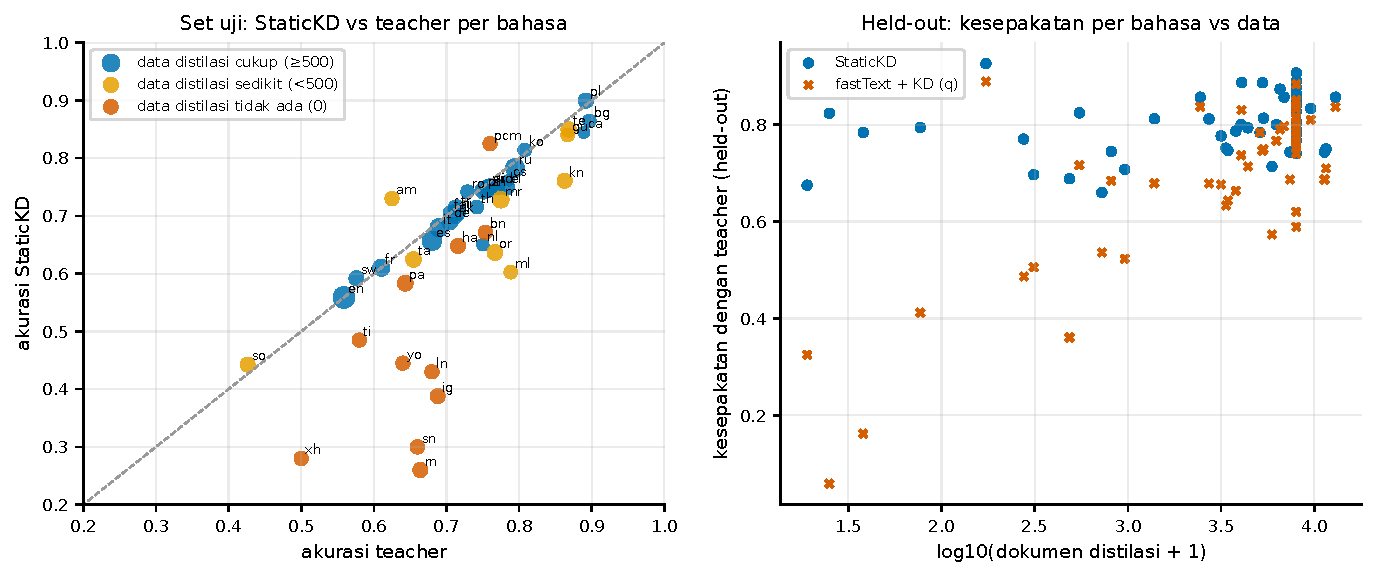
\includegraphics[width=0.9\textwidth]{figures/fig_per_language.pdf}
\caption{Kiri: akurasi StaticKD terhadap akurasi \eng{teacher} per bahasa uji (warna = jumlah data distilasi bahasa, ukuran = jumlah artikel). Kanan: kesepakatan per bahasa \eng{held-out} terhadap jumlah data distilasi, StaticKD vs fastText + KD.}
\label{fig:lang}
\end{figure*}

\textbf{Per label} (Gbr.~\ref{fig:label}).
\begin{itemize}
  \item Label tersulit bagi StaticKD adalah \val{label.hardest}, sedangkan yang termudah \val{label.easiest}.
  \item Selisih terbesar terhadap \eng{teacher} ada pada \val{label.biggest_gap}.
  \item Kebingungan terbesar adalah \val{label.top_confusions}.
\end{itemize}

\begin{figure*}[!t]
\centering
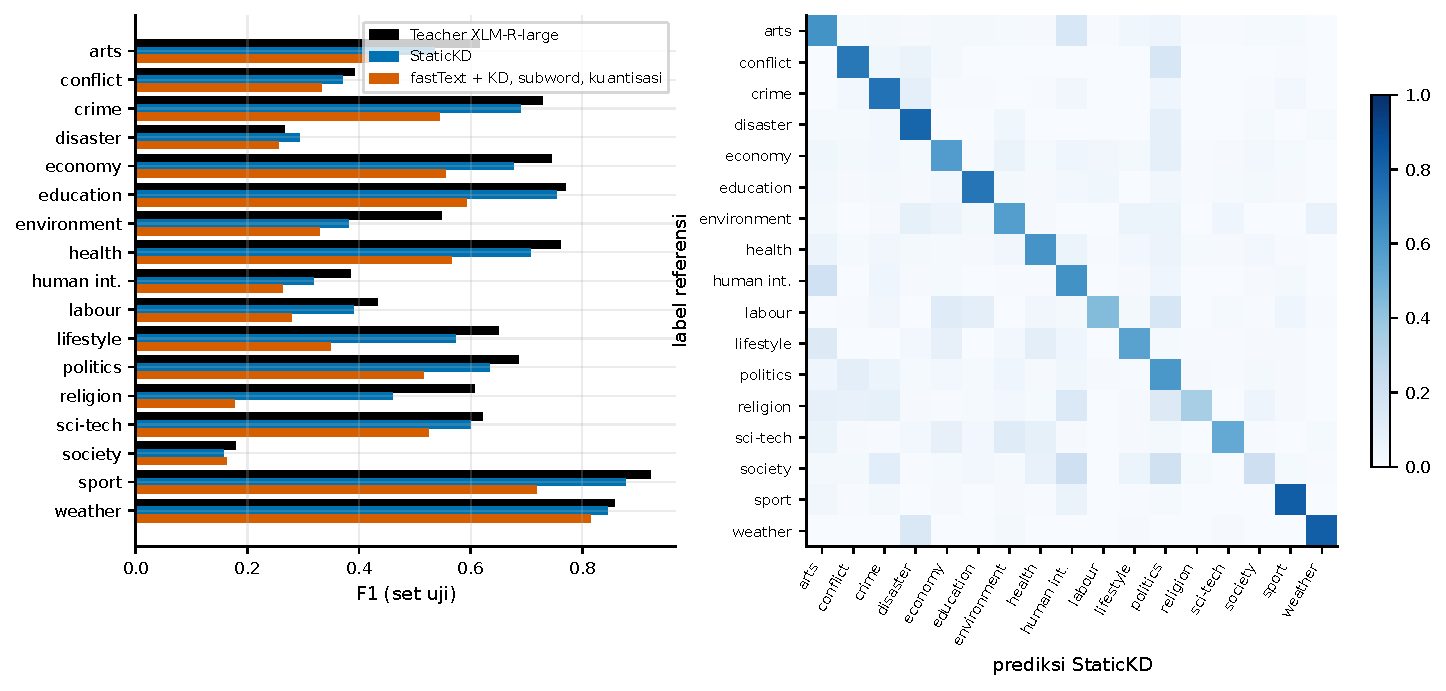
\includegraphics[width=0.9\textwidth]{figures/fig_per_label.pdf}
\caption{F1 per label di set uji (kiri) dan \eng{confusion matrix} StaticKD yang dinormalisasi per label referensi (kanan).}
\label{fig:label}
\end{figure*}

\subsection{Kalibrasi dan Mode \eng{Cascade}}
\TabCascade
\textbf{Kalibrasi.} ECE StaticKD adalah \val{ece.statickd.dev} di dev dan \val{ece.statickd.test} di set uji, lebih rendah daripada ECE \eng{teacher} (\val{ece.teacher.dev} dan \val{ece.teacher.test}). Kedua model menjadi terlalu yakin (\eng{overconfident}) di set uji yang berada di luar distribusi latih (Gbr.~\ref{fig:calib}).

\textbf{\eng{Cascade}.} Artikel dengan keyakinan StaticKD minimal $\theta$ diputuskan oleh StaticKD, dan sisanya dikirim ke \eng{teacher} (Tabel~\ref{tab:cascade}). Dengan $\theta=0{,}8$:
\begin{itemize}
  \item StaticKD memutuskan \val{casc.08.coverage} artikel dengan akurasi \val{casc.08.acc_covered};
  \item akurasi \eng{cascade} keseluruhan menjadi \val{casc.08.accuracy} (\eng{teacher} saja: \val{casc.101.accuracy}) dan macro-F1 \val{casc.08.macro_f1} (\eng{teacher} saja: \val{casc.101.macro_f1});
  \item \eng{throughput} efektifnya \val{casc.08.docs_per_sec} artikel per detik per \eng{core}, dibanding \val{casc.101.docs_per_sec} untuk \eng{teacher} saja.
\end{itemize}
Jadi dengan hanya sekitar dua perlima artikel yang dikirim ke \eng{teacher}, \eng{cascade} menyamai akurasi \eng{teacher}.

\begin{figure}[!t]
\centering
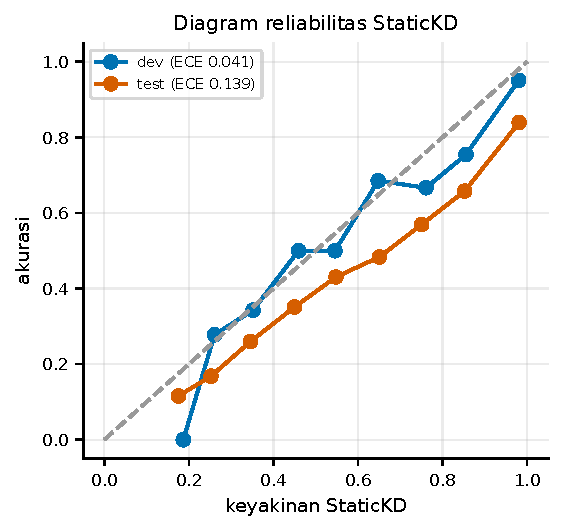
\includegraphics[width=0.8\columnwidth]{figures/fig_calibration.pdf}
\caption{Diagram reliabilitas StaticKD pada dev dan set uji.}
\label{fig:calib}
\end{figure}


% =====================================================================
\section{Pembahasan}
\label{sec:discussion}
\textbf{Tabel token cukup untuk sebagian besar topik berita (RQ1, RQ2).} StaticKD mempertahankan \val{statickd.test.pct_teacher} macro-F1 \eng{teacher} di set uji gabungan dan \val{statickd.dev.pct_teacher} di dev, dengan biaya inferensi dua sampai tiga orde besaran lebih rendah (\val{eff.statickd.speedup_onnx}$\times$ terhadap ONNX int8, \val{eff.statickd.speedup_pt}$\times$ terhadap PyTorch). Hal ini konsisten dengan temuan bahwa representasi tanpa urutan kata sudah kompetitif untuk klasifikasi topik~\cite{galke2022bow,iyyer2015dan}: nama lembaga, istilah olahraga, dan kosakata medis membawa sebagian besar sinyal topik. Sisa kesenjangan terkonsentrasi di dua tempat.
\begin{itemize}
  \item Label yang kosakatanya tumpang tindih dengan topik lain. Selisih terbesar terhadap \eng{teacher} ada pada \val{label.biggest_gap}. Label tersulit bagi StaticKD (\val{label.hardest}) juga termasuk yang tersulit bagi \eng{teacher} (Gbr.~\ref{fig:label}). \eng{Society} dan \eng{human interest} juga dikenal sulit bagi anotator manusia~\cite{kuzman2025llm}.
  \item Bahasa yang kurang terwakili di data distilasi. Pada bahasa dengan data distilasi cukup, StaticKD mencapai \val{grp.distil_tier.cukup.pct} skor \eng{teacher}; pada bahasa tanpa data distilasi, \val{grp.distil_tier.tidakada.pct}.
\end{itemize}
Dengan data distilasi yang sama, MiniLM-L6 menutup sebagian kesenjangan tersebut (selisih StaticKD $-$ MiniLM \val{sig.test.minilm_kd.delta}, $p$ \val{sig.test.minilm_kd.p}). DistilmBERT tidak menutupnya (selisih StaticKD $-$ DistilmBERT \val{sig.test.distilmbert_kd.delta}, $p$ \val{sig.test.distilmbert_kd.p}). Keduanya membutuhkan biaya satu sampai dua orde besaran lebih tinggi. Ini menunjukkan bahwa kualitas representasi multibahasa awal lebih menentukan daripada jumlah \eng{layer}: MiniLM berasal dari XLM-R-large, sedangkan DistilmBERT dari mBERT.

\textbf{Dari mana pengetahuan \eng{student} berasal (RQ3).} Ablasi memisahkan tiga sumber.
\begin{enumerate}
  \item \textbf{Data distilasi multibahasa yang dilabeli \eng{teacher}} adalah faktor terbesar. Tanpa data ini, macro-F1 uji turun sebesar \val{abl.emm_only.test_macro.delta}. Temuan ini sejalan dengan pandangan klasik bahwa nilai distilasi terletak pada \eng{transfer set} berlabel \eng{teacher}~\cite{bucilua2006model,ye2022sparse}.
  \item \textbf{Inisialisasi embedding yang selaras lintas bahasa.} Inisialisasi acak mengubah macro-F1 uji sebesar \val{abl.random_init.test_macro.delta}. Bukti yang lebih langsung datang dari varian \eng{compact}. Pada bahasa India yang hampir tidak ada di data distilasi (misalnya bn, pa, or), sebagian besar token tidak pernah diperbarui saat \eng{training}, sehingga embedding-nya tetap embedding awal potion. Meski begitu, StaticKD tetap mengklasifikasikan bahasa-bahasa ini dengan cukup baik (akurasi rata-rata \val{lang.vlowcov.static_acc}; Gbr.~\ref{fig:lang}). Ketika token-token tersebut dibuang oleh pemangkasan tokenizer, akurasinya jatuh ke \val{lang.vlowcov.compact_acc}. Jadi transfer ke bahasa tanpa data dibawa oleh baris embedding yang \emph{tidak pernah dilatih}, tetapi berada dalam ruang yang sama dengan baris yang dilatih. Kepala linear yang dipelajari dari bahasa kaya data berlaku juga untuk baris-baris ini.

  Ablasi embedding beku memperlihatkan sisi lain dari mekanisme yang sama. \eng{Fine-tuning} menggeser embedding token dari bahasa yang ada di data distilasi. Akibatnya kecocokan in-distribusi naik (dev \val{abl.frozen.dev_macro.delta} bila dibekukan), tetapi token bahasa lain tertinggal di ruang potion yang asli, sehingga kepala linear yang sudah menyesuaikan diri dengan ruang baru kurang cocok untuk token-token itu. Di bahasa tanpa atau dengan sedikit data distilasi, embedding beku lebih baik sebesar \val{ablgrp.frozen.tidakada.delta} dan \val{ablgrp.frozen.sedikit.delta}. Ini adalah bentuk pergeseran representasi (\eng{representation drift}) akibat \eng{fine-tuning} pada sebagian kosakata. Resep final tetap memakai \eng{fine-tuning} karena resep dipilih pada set \eng{development} yang berbahasa latih. Namun untuk penggunaan yang menargetkan bahasa tanpa data distilasi, varian beku atau regularisasi yang menahan embedding dekat ke potion adalah pilihan yang lebih aman. Keduanya tetap dapat dilipat menjadi tabel.
  \item \textbf{\eng{Soft label} memberi manfaat kecil atau tidak ada.} Label keras \eng{teacher} tidak berbeda signifikan dari \eng{soft label} dengan $\tau=1$ (dev \val{abl.hard.dev_macro.delta}, uji \val{abl.hard.test_macro.delta}). Sebaliknya, $\tau=2$ menurunkan kesepakatan \eng{held-out} dan macro-F1 uji, dan $\tau=4$ menurunkan semua metrik. Temuan ini sejalan dengan literatur \eng{capacity gap}~\cite{cho2019efficacy,zhang2025law,wang2026rckd}. \eng{Student} yang hanya berupa satu lapisan linear di atas rata-rata embedding tidak mampu merepresentasikan struktur antarkelas dalam ekor distribusi \eng{teacher} (\eng{dark knowledge})~\cite{zhao2022dkd,huang2022dist}. Distribusi yang lebih tajam ($\tau=1$) atau label keras memberi target yang dapat dicapai, sedangkan $\tau$ tinggi memaksa \eng{student} meniru skala dan bentuk logit yang di luar kapasitasnya~\cite{sun2024logit}.
\end{enumerate}
Kesimpulan praktisnya: untuk \eng{student} berkapasitas sangat rendah, sumber daya sebaiknya diarahkan ke cakupan \eng{transfer set} (bahasa, situs, topik) dan inisialisasi yang selaras, bukan ke penyetelan bentuk \eng{soft label}.

\textbf{Batas generalisasi lintas bahasa (RQ4).} Kinerja per bahasa terutama ditentukan oleh keterwakilan bahasa di data distilasi dan di pra-latih, bukan oleh sistem tulisan (Kruskal--Wallis $p$ \val{fac.kw.p}). Kelemahan terbesar ada pada bahasa Afrika yang berada di luar pra-latih XLM-R dan tidak ada di data distilasi (\val{lang.outxlmr.langs}). Pada bahasa-bahasa ini \eng{teacher} masih cukup kuat (akurasi \val{lang.outxlmr.teacher_acc}), mungkin berkat subword yang dipakai bersama dengan bahasa lain dan konteks kalimat, sedangkan StaticKD jauh lebih lemah (\val{lang.outxlmr.static_acc}). Solusi termurahnya tidak memerlukan perubahan arsitektur: tambahkan berita dalam bahasa-bahasa tersebut ke \eng{transfer set} dan biarkan \eng{teacher} melabelinya. Ablasi data dan korelasi kesepakatan dengan jumlah data ($\rho=\val{fac.data.rho}$) mendukung saran ini.

\textbf{\eng{Fidelity} tidak sama dengan akurasi.} Beberapa varian menggerakkan kesepakatan dengan \eng{teacher} dan akurasi terhadap label independen ke arah yang berlawanan.
\begin{itemize}
  \item Embedding beku menurunkan kesepakatan \eng{held-out} (\val{abl.frozen.heldout_acc.delta}) tetapi menaikkan macro-F1 uji (\val{abl.frozen.test_macro.delta}).
  \item Mengurangi data ke 130 ribu dokumen menurunkan kesepakatan (\val{abl.data130k.heldout_acc.delta}) tanpa perubahan signifikan di set uji (\val{abl.data130k.test_macro.delta}).
\end{itemize}
Sejalan dengan~\cite{stanton2021kd,ojha2023knowledge}, pemilihan \eng{student} sebaiknya memakai label yang independen dari \eng{teacher} dan set uji di luar distribusi latih, bukan \eng{fidelity} saja.

\textbf{Posisi terhadap penelitian sebelumnya.}
\begin{itemize}
  \item Dibanding \eng{Sparse Distillation}~\cite{ye2022sparse}, StaticKD mengganti tabel n-gram yang dilatih dari nol dengan embedding multibahasa pra-latih yang dilipat ke 17 logit per token. Model menjadi jauh lebih kecil dan dapat ditransfer ke bahasa yang tidak ada di \eng{transfer set}.
  \item Dibanding KD-LoRA dan PEFT~\cite{azimi2024kdlora,razuvayevskaya2024peft}, StaticKD menurunkan biaya inferensi, bukan biaya \eng{training}. Untuk \eng{pipeline} berita, biaya inferensi inilah yang dominan~\cite{luccioni2024power}.
  \item Kuantisasi int8 \eng{teacher} hanya memberi percepatan dengan faktor konstan~\cite{yao2022zeroquant}.
\end{itemize}

\textbf{Implikasi praktis.}
\begin{itemize}
  \item Untuk \eng{pipeline} \eng{real-time} di server tanpa GPU, StaticKD memproses satu juta artikel per hari dengan \val{eff.statickd.cores1M} \eng{core}, file \val{final.size}~MB, dan dependensi hanya \texttt{numpy} dan \texttt{tokenizers}.
  \item Probabilitas StaticKD lebih terkalibrasi daripada \eng{teacher} (ECE uji \val{ece.statickd.test} vs \val{ece.teacher.test}), sehingga dapat dipakai untuk mode \eng{cascade}. Dengan $\theta=0{,}8$, \val{casc.08.coverage} artikel diputuskan StaticKD dan sisanya dikirim ke \eng{teacher}. Akurasi keseluruhannya (\val{casc.08.accuracy}) setara dengan \eng{teacher} saja (\val{casc.101.accuracy}), dengan \eng{throughput} \val{casc.08.docs_per_sec} artikel per detik per \eng{core}, dibanding \val{eff.teacher_onnx_int8.docs_per_sec_1c} untuk \eng{teacher} saja. Mode ini cocok untuk jalur \eng{batch} yang membutuhkan akurasi setara \eng{teacher}.
  \item Varian \eng{compact} menurunkan RAM, tetapi hanya layak bila semua bahasa sasaran tercakup data distilasi.
\end{itemize}


% =====================================================================
\section{Keterbatasan}
\label{sec:limitations}
\begin{enumerate}
  \item \textbf{Label silver.} Sebanyak \val{ts.origin.publisher_section_jsonld.pct} artikel set uji berlabel rubrik JSON-LD dan \val{ts.origin.publisher_category.pct} berlabel kategori penerbit. Pemetaannya konservatif dan tervalidasi terhadap pohon IPTC, tetapi tidak dianotasi ulang oleh manusia. Pemeriksaan tidak langsung pada Subbagian~\ref{sec:res-validity} menunjukkan bahwa, di bahasa yang sama, kesepakatan \eng{teacher} dengan label silver tidak lebih rendah daripada dengan label manusia. Walau begitu, skor absolut pada label silver sebaiknya dibaca sebagai estimasi yang mengandung derau, terutama untuk label yang batasnya kabur (\eng{society}, \eng{human interest}, \eng{lifestyle}).
  \item \textbf{Label MasakhaNEWS dianotasi manusia dengan skemanya sendiri}, lalu dipetakan ke IPTC. Hanya MN-DS yang dianotasi langsung dengan topik IPTC, dan dataset itu hanya berbahasa Inggris. \eng{Test set} manusia IPTC multibahasa dari Kuzman dan Ljube\v{s}i\'c~\cite{kuzman2025llm} tidak publik, sehingga tidak dipakai.
  \item \textbf{Cakupan label per bahasa timpang.} Median jumlah label per bahasa adalah \val{ts.lang_labels.median}. Bahasa Afrika hanya mencakup empat sampai lima topik besar. Macro-F1 dihitung atas label yang hadir, sehingga skor per bahasa tidak dapat dibandingkan secara langsung antarbahasa dengan cakupan label berbeda.
  \item \textbf{Keragaman penerbit terbatas pada sebagian bahasa.} Sebanyak \val{ts.div.satu.langs} bahasa praktis berasal dari satu penerbit: BBC/VOA untuk bahasa Afrika, L3Cube untuk bahasa India, dan satu situs untuk beberapa bahasa CC-NEWS. Klaim untuk bahasa-bahasa ini terbatas pada penerbit tersebut. \eng{Site-cluster bootstrap} memperlebar interval kepercayaan sesuai kondisi ini.
  \item \textbf{Batas atas \eng{student} adalah \eng{teacher}.} Kesalahan dan bias \eng{teacher} ikut tertiru. Set \eng{fidelity} mengukur kemiripan dengan \eng{teacher}, bukan kebenaran.
  \item \textbf{Satu perangkat \eng{benchmark}.} Angka absolut di server akan berbeda, tetapi rasio antarmodel yang diukur dalam sesi dan protokol yang sama tetap informatif.
  \item \textbf{Keadilan antarbahasa dan dampak.} Akurasi StaticKD jauh lebih rendah pada bahasa Afrika yang tidak terwakili di data distilasi maupun pra-latih (Subbagian~\ref{sec:discussion}). Karena itu, penerapan sebagai penyaring topik dapat membuat berita dalam bahasa-bahasa ini lebih sering salah dikategorikan atau terbuang. Kami menyarankan agar akurasi dipantau per bahasa sebelum model dipakai, dan agar artikel berkeyakinan rendah dikirim ke \eng{teacher} lewat mode \eng{cascade}.
  \item \textbf{Cakupan tugas.} Penelitian ini hanya mencakup label IPTC level atas dan klasifikasi \eng{single-label}. Level yang lebih dalam dan artikel multi-topik belum diuji.
\end{enumerate}


% =====================================================================
\section{Kesimpulan}
\label{sec:conclusion}
Penelitian ini mengukur biaya CPU pengklasifikasi IPTC multibahasa terbuka dan menunjukkan bahwa biayanya dapat diturunkan dua sampai tiga orde besaran (terhadap \eng{teacher} ONNX int8 dan PyTorch) sambil mempertahankan sebagian besar akurasinya. StaticKD mendistilasi \eng{teacher} XLM-R-large ke tabel 17 logit per token. Tabel ini diinisialisasi dari \eng{static embedding} multibahasa dan dilatih pada \val{data.pool.docs} artikel dari \val{data.pool.langs} bahasa yang dilabeli \eng{teacher}.
\begin{itemize}
  \item Pada set uji gabungan (\val{ts.docs} artikel, \val{ts.langs} bahasa) yang labelnya independen dari \eng{teacher}, StaticKD mencapai macro-F1 \val{statickd.test.macro}, atau \val{statickd.test.pct_teacher} dari \eng{teacher}.
  \item Kecepatannya \val{eff.statickd.docs_per_sec_1c} artikel per detik per \eng{core} CPU, sekitar \val{eff.statickd.speedup_onnx} kali lebih cepat dari \eng{teacher} ONNX int8, dengan model \val{final.size}~MB tanpa pustaka \eng{deep learning}.
  \item Kunci keberhasilannya adalah \eng{transfer set} multibahasa dan embedding yang selaras lintas bahasa. Pada \eng{student} berkapasitas sangat rendah, \eng{soft label} dan \eng{temperature} tinggi tidak memberi manfaat, sedangkan \eng{ensemble} beberapa \eng{seed} dapat dilipat menjadi satu tabel tanpa biaya.
  \item \eng{Fine-tuning} embedding menaikkan akurasi pada bahasa yang ada di data distilasi, tetapi menurunkannya pada bahasa tanpa data distilasi. Transfer ke bahasa-bahasa tersebut dibawa oleh embedding pra-latih yang tidak ikut dilatih.
  \item Set uji dengan pemetaan rubrik ke pohon IPTC, kontrol kontaminasi, dan \eng{site-cluster bootstrap} dapat dipakai ulang untuk mengevaluasi pengklasifikasi IPTC lain.
\end{itemize}

Penelitian lanjutan mencakup:
\begin{itemize}
  \item memperluas \eng{transfer set} ke bahasa yang lemah, terutama bahasa Afrika di luar pra-latih XLM-R;
  \item regularisasi \eng{fine-tuning} yang menahan embedding dekat ke ruang pra-latih, supaya akurasi in-distribusi dan transfer lintas bahasa dapat diperoleh bersamaan;
  \item kepala non-linear yang tetap murah dengan embedding terkuantisasi, mengingat kepala MLP memberi kenaikan kecil;
  \item tokenizer yang lebih cepat (misalnya pencarian kata langsung ke tabel), karena tokenisasi mengambil \val{prof.statickd.tokshare} waktu inferensi;
  \item pemangkasan tokenizer yang mempertahankan token lintas bahasa;
  \item klasifikasi hierarkis ke IPTC level 2 dan klasifikasi multi-label;
  \item validasi dengan anotasi manusia IPTC multibahasa pada sampel set uji.
\end{itemize}


% =====================================================================
\section*{Ketersediaan Kode, Model, dan Data}
Kode (pengumpulan data, konstruksi set uji, pelabelan \eng{teacher}, \eng{training}, evaluasi, \eng{benchmark}) dan notebook yang mereproduksi setiap angka, tabel, dan gambar naskah ini tersedia di \todo{URL GitHub}. Model StaticKD tersedia di \todo{URL Hugging Face}. Set uji dirilis sebagai manifest berisi URL/ID artikel, label, dan asal label, beserta skrip rekonstruksi. Teks artikel tidak dirilis ulang karena hak cipta penerbit dan lisensi dataset sumber (misalnya CC BY-NC untuk MasakhaNEWS). EMMediaTopic tersedia di CLARIN.SI.

\section*{Pernyataan Penggunaan AI}
\todo{Sesuaikan dengan kebijakan jurnal.} Penulis menggunakan asisten AI (Claude, Anthropic) untuk membantu penulisan kode eksperimen, analisis, dan penyusunan draf naskah. Seluruh desain, hasil, dan klaim telah diperiksa dan menjadi tanggung jawab penulis.

\section*{Ucapan Terima Kasih}
\todo{Pembimbing, pendanaan, fasilitas.}

\bibliographystyle{IEEEtran}
\bibliography{references}

\end{document}
